% Draft Version 1 - Date 16/06/2020
% Draft Version 2 - Date 06/08/2020
% Draft Version 3 - Date 27/08/2020
% Draft Version 4 - Date 14/12/2020
\chapter{\titlenn}\label{chap-nn}

\section{Introduction}
Considering the fact that DNS simulations of heterogeneous media are computationally hard to deal with, one can employ a computational multi-scale scheme such as multilevel finite element method (FE$^\text{2}$)\cite{feyelMultilevelFiniteElement2003} as presented in Chapter \ref{chap-ch}. But yet, the computational bottleneck in these methods, which is the iterative evaluation of the micro model Boundary value problem (BVP) at each integration point in the macro-model makes the methodology computationally expensive to be employed in many-query applications. 

\red{There are various methodologies that have been developed to find a cost vs accuracy balance. For example, the analytical micro-mechanical methods\cite{eshelbyDeterminationElasticField1957,liuDevelopmentStrategyRestructuring2015,hillSelfconsistentMechanicsComposite1965,hashinVariationalApproachTheory1963} uses several micro-structural descriptors to describe the heterogeneous material. While this makes the methods efficient, they are based on mean-field assumptions, limiting their applicability to complex micro-structures and localized plastic behavior. The nonuniform transformation field analysis (NTFA)\cite{michelNonuniformTransformationField2003} leverages the capabilities of the analytical micro-mechanical methods and subjects the input variables to so called evolution equations. This method, while keeping the computational cost low, requires the inclusion of empirical laws that requires further calibration. Further, to obtain the plastic modes, extensive irreversible deformations at the offline stage needs to be conducted.}

Reduced order modeling (ROM) technique involves the reduction of the model complexity of the microscopic boundary value problem (BVP) by the support of a series of analysis snapshots that are obtained before the model development in a stage known as offline training. The ROM solutions belonging to reduced manifolds are sought with the help of projection constraints based on the governing equations. These reduced versions are extracted during the offline training by the projections based on the number of displacement degrees of freedom by proper generalized decomposition (PGD) methods within a parametric stochastic network\cite{chevreuilModelOrderReduction2012} and a hyper reduced model on the basis of internal forces\cite{hernandezDimensionalHyperreductionNonlinear2017} ending up in a dramatic reduction in the number of degrees of freedom along with the required computations of the constitutive model all while ensuring increased accuracy and efficiency. Proper orthogonal decomposition (POD)\cite{yvonnetReducedModelMultiscale2007} defines the principal modes by using the linear combinations of all input variables, but makes this method quite expensive computationally. PGD in combination with \fee multi-scale simulations has been studied in \cite{bhattacharjeeNonlinearManifoldbasedReduced2016} with the macro-scale simulations coupled with the resolution of the ROM equations. But this compromise to save time may not always justify these complex multi-scale simulations using ROM. This brings focus on novel techniques that can be used as surrogates to help overcoming the handicaps of the method or alleviate the problems of computational cost brought forward by the method without sacrificing the generality presented by \fee. 

Machine learning is the scientific discipline that seeks to understand and improve how computers learn from data. As such, it combines elements from statistics with the understanding of relationships from data, and with elements from computer science by developing algorithms to manage data. The success of this discipline relies heavily on the ability to collect and interpret the data \cite{pengMultiscaleModelingMeets2020}. When the goal is to reveal correlation features and where the answer is binary, machine learning techniques are exceptionally good at integrating these multi-modal multi-fidelity based data \cite{krizhevskyImageNetClassificationDeep2012}. However, problems might arise while dealing with sparse or biased data \cite{rileyThreePitfallsAvoid2019} that can result in their naive use on ill posed problems and then to generate non-physical predictions. Recent trends in computational physics suggest that on the basis of the knowledge of the underlying physics, the prior knowledge can then be integrated to constrain the space of admissible solutions to a manageable size \cite{bruntonDiscoveringGoverningEquations2016, raissiPhysicsinformedNeuralNetworks2019}, or used in the generation of synthetic data on the basis of multi-scale modeling and physics based simulation\cite{contiDataDrivenProblemsElasticity2018}. With the availability of modern computation facilities, that are not just powerful but also affordable, this generated database can be used to enhance the knowledge about the materials and the underlying physics behind their behavior.

\red{The evaluation of material response, possibly by homogenization, can also be replaced completely by already taking into account the prior knowledge about the physics behind these evaluations and by then employing data-driven methods as the surrogate models. Some of them include principal component analysis\cite{hottaRobustFaceRecognition2008,liKPCASemanticObject2008}, kernel methods\cite{nowickiDatadrivenModelsFault2012}, and artificial neural networks (ANN)\cite{lefikArtificialNeuralNetwork2003} that have gained momentum and popularity due to the aforementioned computational reasons. In particular, ANNs have the  capability to approximate any continuous function to any level of precision making them a good general approximator in the given training range, while depending on the freedom to parameterize and the settings to train these models \cite{cybenkoApproximationSuperpositionsSigmoidal1989}. For example, in \cite{ghaboussiAutoprogressiveTrainingNeural1998}, a fixed macroscopic strain distribution enabled improved predictions by restricting the parameter space. Further, a full micro-scale model can be used to generate snapshots of the homogenized states, which can then be used to train ANNs, followed by their use in an online scheme to predict stress and tangent stiffness. Authors in \cite{leComputationalHomogenizationNonlinear2015} introduced additional micro-structure parameters, besides the homogenized strain, into the network input space, in order to predict the elastic energy from which the homogenized stress can be derived, while \cite{luDatadrivenComputationalHomogenization2018} attempted introducing physics based constraints showing that with the availability of the extensive amount of data and the computational prowess, ANN based models are a perfect fit in the progress of increasing the computational speed of \fee analysis. A history dependent ANN surrogate has been presented in \cite{ghavamianAcceleratingMultiscaleFinite2019} with the help of gated layers in a process that resembles classical nonlinear finite element analysis in an offline training stage.}

\red{This work presents a critical comparison of the use of different ANN architectures to represent the material response. By applying this methodology on history dependent behavior of the micro-structure, the approach covers a large aspect of the plastic behavior of such materials.}

In this chapter, a study on the implementation of ANN based models on 2D open foam-like geometries is presented. A basic information about various ANNs like Feedforward neural networks (FNNs) and recurrent neural networks (RNNs) is presented. An initial study on the predictability of ANNs on monotonic behavior is then expanded to study history dependent behavior while discussing the limitations of such expansions. Suitable adjustments and modifications necessary, such as the implementation of RNNs, that is necessary to understand the increased amount of data that history dependent behavior might demand, is presented. To aid in this approach, a state based representation scheme of the material is presented to be applied in a two stage FNN based approach. A clustering scheme is also studied and has been expanded to the two stage FNN based approach to understand the relation between the amount of data and the accuracy of ANN predictions. 


\section{Introduction to Artificial Neural Networks (ANN)}\label{nn-ann}

ANNs are machine learning models inspired from the functioning and structuring of a biological brain. The data structures and the functionalities of the ANNs are designed to ensure a process of simulating associative memory. By performing probability-weighted associations between any given input set and its intended result set, ANNs are expected to ``learn" and store these associations within the data structure of the network itself. The ``learning" is signified by the resulting difference in the state of the network before and after the training process. A feedback loop can be used to refine the associations formed by improving over the accuracy of its predictions. Thus, by ensuring a diversity and the number of training examples, the network can be made capable of predicting results from inputs. 

The ANNs are expected to simply perform a function
\begin{equation}\label{eq-nn-func}
\mathcal{F}\colon\textbf{\textit{u}}\to\textbf{\textit{v}}
\end{equation}
with $ \textbf{\textit{u}}=[u_1\,u_2\,...\,u_{n_0}]^T $ and $ \textbf{\textit{v}}=[v_1\,v_2\,...\,v_{n_N}]^T $, where $ \textbf{\textit{u}}\in\mathbb{R}^{n_0} $ and $ \textbf{\textit{v}}\in\mathbb{R}^{n_N} $. These networks are made of individual computational units called nodes or neurons that receive inputs along the incoming edges, then multiply the inputs by a corresponding edge weights, and finally apply a non-linear function called an activation function, $ \phi $, before producing an output using the output function, $ f $. This weighted sum operation of a neuron, $ j $, can be represented as 
\begin{equation}\label{eq-nn-weight}
v_j(u_1,...,u_{n_0})=f_j(u_1,...,u_{n_0},w_0,...,w_{n_0})=\phi_j(w_0+\sum_{k=1}^{n_0}w_ku_k).
\end{equation}
with the weights $ w_{k} $, $ k=1,...,n_0 $, and the bias term $ w_{0} $ (Figure \ref{fig-nn-nnw}a).

\begin{figure}
	\centering
	\begin{subfigure}[t]{0.45\textwidth}
		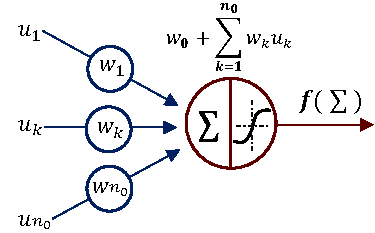
\includegraphics[width=\textwidth]{NNW_a}
		\caption{}
	\end{subfigure}
	\begin{subfigure}[t]{0.45\textwidth}
		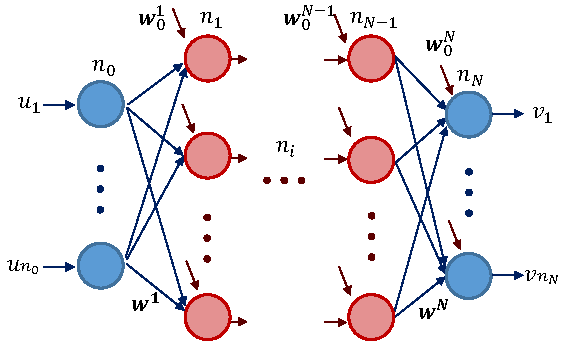
\includegraphics[width=\textwidth]{NNW_b}
		\caption{}
	\end{subfigure}
	\caption{(a) Functioning of an artificial neuron, and (b) a simple feed-forward neural network with an input layer having $ n_0 $ inputs and an output layer having $ n_N $ outputs connected by a set of $ n_{N-1} $ hidden layers\cite{wuRecurrentNeuralNetworkaccelerated2020}. }\label{fig-nn-nnw}
\end{figure}

The activation function introduces non-linearities in the system while propagating the state of the neuron between various layers of the network. A standard activation function used is the sigmoid function,
\begin{equation}\label{eq-nn-sigmoid}
\phi_{SIG}(\nu)=\frac{\text{e}^\nu}{\text{e}^\nu+1},
\end{equation}
which is applied element wise before propagating the state of the neuron down the network. Sigmoid functions remain a popular choice for building regression models\cite{leComputationalHomogenizationNonlinear2015}. Another option is a leaky rectified linear unit (Leaky ReLU) activation\cite{liuModifiedLeakyReLU2019} that can be represented as
\begin{equation}\label{eq-nn-lrelu}
\phi_{LR}(\nu)=
\begin{cases}
\nu,\quad \nu\ge0\\
\epsilon\nu,\quad \nu<0
\end{cases}
\end{equation}
where $ \epsilon $ is a small number. These are further described briefly in Appendix \ref{app-act}.

In this section, a brief introduction is provided on the FNNs and multi-layer perceptron (MLP), the most common FNN along with the methodology of training the ANNs on the basis of backpropagation, and the testing and validation of the ANNs. A brief summary on the RNNs is provided to form the basis for the history-dependent behavior analysis with the help of the internal states stored in the RNN modules. This is followed by a double feedforward neural network (\fnn)\cite{nguyenSurrogateModelsBasedUnderPreparation} that mimics the internal states present in RNN modules.

\subsection{Feedforward Neural Network (FNN)}\label{nn-ann-stru}
An FNN is one of the simplest form of ANNs where the information moves only in one direction, from the input nodes, through any hidden nodes and to the output nodes in the forward direction. Generally these networks do not have any loops or cycles. The simplest form of such a network is the single-layer perceptron where a single layer accepts the input, applies the weights and gives the output after the application of an activation function\cite{kellerFiniteAutomataPattern1961}. These networks are capable of learning only the linearly separable patterns that lie underneath the given data although these can approximate any continuous functions when dealing with real numbers in the interval [-1,1]\cite{auerLearningRuleVery2008}.

A multi-layer perceptron (MLP) consists of multiple layers of computational neurons that are connected in a feed-forward way. The neurons in one layer are connected to the neurons of the subsequent layer\cite{hastieElementsStatisticalLearning2009}. An MLP can be simply made of an input layer, one hidden layer and an output layer, such networks colloquially referred to as ``vanilla" networks. Except the input nodes, each node on the network is a neuron where a nonlinear activation function can be applied. These introduced non-linearities give the network the ability to distinguish data that is not linearly separable. MLPs can be trained using a supervised training technique called back-propagation.

Figure \ref{fig-nn-nnw}b illustrates a classical FNN with $ N-1 $ hidden layers in between the input layer and the output layer. The weights matrix of a layer $ i $, $ \textit{\textbf{w}}^i $ is made of components $ w^i_{kj} $, with the layer denoted by $ i=1,...,N $, a node in the layer $ i-1 $ denoted by $ k=1,...,n_{i-1} $ and a neuron in the current layer $ i $ denoted by $ j=1,...,n_i $, and thus $ \textbf{\textit{w}}^i\in\mathbb{R}^{n_{i-1}\times n_i} $. The bias vector $ \textit{\textbf{w}}^i_0 $ for the layer is made of components $ w^i_{0j} $, and thus $ \textbf{\textit{w}}^i_0\in\mathbb{R}^{n_i} $. The weights matrices, $ \textbf{\textit{w}}^i $, and the bias vectors, $ \textbf{\textit{w}}^i_0 $, together constituting the model parameters, can be represented in a tensorial form as $ \textbf{W} $, so that the mathematical model of an ANN can be written as 
\begin{equation}\label{eq-nn-nnw}
\textit{\textbf{v}}=\mathcal{F}(\textit{\textbf{u}},\textbf{W}).
\end{equation} 

In this work, FNN models will be used to study the training, validating and testing of ANN as surrogates for micro-scale BVP when the loading pattern is monotonic in nature.

\subsection{Training of ANNs}\label{nn-ann-train}

The model parameters, $\textbf{W} $ need to be trained in an offline stage so that the ANN can be effectively used to predict the necessary outputs. The neurons of the layers of the FNN propagate the states of the neurons $ \textbf{\textit{a}} $, which can simply be considered as activated (or 1) or deactivated (or 0), from the previous layer, $ i-1 $, to the subsequent layer, $ i $, by applying the set of activation functions\footnote{The most basic form of activation, step activation (Appendix \ref{app-act}), works like a switch that receives and outputs only the presence (or 1) or absence (or 0) of a signal. In general, however, the neurons propagate a continuous floating point value depending on the activation functions used.}, $ \bm\phi_{i}=[\phi_1,...,\phi_{n_{i}}] $, neuron-wise on the entire layer, which can be represented as
\begin{equation}\label{eq-nn-state}
\textbf{\textit{a}}_i=\bm\phi_{i}\left(\textbf{\textit{w}}^i\textbf{\textit{a}}_{i-1}+\textbf{\textit{w}}_0^i\right).
\end{equation}

The distance between the network output and the desired output can be measured using a loss function during the training process and an optimization algorithm is used to evaluate $ \textbf{W} $. A commonly used loss function for a regression problem, where a continuous value is to be predicted, is the mean square error (MSE). The error or residual in general is represented by $ L(\textbf{W}) $ with the $ p $-Frobenius norm
\begin{equation}\label{eq-nn-loss}
L(\textbf{W})=\left(\frac{1}{N_{obs}}\sum_{l=1}^{N_{obs}}\left|\left|\mathcal{F}(\textbf{\textit{u}}_l,\textbf{W})-\hat{\textbf{\textit{v}}}_l\right|\right|^p\right)^{\frac{1}{p}}
\end{equation}
with the number of input-output observations $ N_{obs} $, and $ \hat{\textbf{\textit{v}}_l} $ the actual output. For MSE, this is 
\begin{equation}\label{eq-nn-mse}
L_{MSE}(\textbf{W})=\left(\frac{1}{N_{obs}}\sum_{l=1}^{N_{obs}}\left({\mathcal{F}(\textbf{\textit{u}}_l,\textbf{W})-\hat{\textbf{\textit{v}}}_l}\right)^2\right)^\frac{1}{2}.
\end{equation}

A Stochastic Gradient Descent (SGD) optimization algorithm can be then used on the objective function $ L $ to update $ \textbf{W} $. Thus
\begin{equation}\label{eq-nn-sgd}
\textbf{W}^t=\textbf{W}^{t-1}-\mathcal{A}\left(\frac{1}{N_{batch}}\sum_{j=1}^{N_{batch}}\frac{\partial L_j}{\partial\textbf{W}}\right)
\end{equation}
with the operator $ \mathcal{A} $ that depends on the choice of the solver, $ t-1 $ and $ t $ denoting the previous and current values, the loss term $ L_j $ of the $ j $-th sample, and the mini-batch size $ N_{batch} $ used during the update. The division of the sample into mini-batches balances the speed of convergence and the gradient variance. So, an epoch, or one iteration of the solving procedure, is said to be complete only when the model has seen all the samples $ N_{obs} $ that exist in the training set, or after $ {N_{obs}}/{N_{batch}} $ mini-batches. A common choice for the operator $ \mathcal{A} $ is Adam solver that is based on adaptive estimates of lower-order moments\cite{kingmaAdamMethodStochastic2014}.

The gradients in Eq. (\ref{eq-nn-sgd}) can be computed by a back-propagation procedure that propagates the loss function from output layer progressively towards the beginning of the network using the chain rule. This can be summarized in the following manner:
\begin{itemize}
	\item Initialize an auxiliary quantity $ \textbf{\textit{d}}_{N-1}\in\mathbb{R}^{n_{N-1}} $ at the output layer, $ N-1 $, as
	\begin{equation}\label{eq-nn-sgd1}
	\textbf{\textit{d}}_{N-1}=\frac{\partial L}{\partial\textbf{\textit{a}}_{N-1}},
	\end{equation}
	and consider $ i=N-1 $;
	\item Apply the effect of activation function
	\begin{equation}\label{eq-nn-sgd2}
	\bar{\textbf{\textit{d}}}_i=\textbf{\textit{d}}_i\odot\frac{\partial\bm\phi}{\partial\nu}(\textbf{\textit{w}}^i\textit{\textbf{a}}_{i-1}+\textbf{\textit{w}}^i_0)
	\end{equation}
	using element-wise multiplicator $ \odot $;
	\item Compute gradients of trainable parameters
	\begin{equation}\label{eq-nn-sgd3}
		\frac{\partial L}{\partial\textbf{\textit{w}}^i} = \bar{\textbf{\textit{d}}}_i\textbf{\textit{a}}_i^T,
	\end{equation}
	and
	\begin{equation}
		\frac{\partial L}{\partial\textbf{\textit{w}}^i_0} = \bar{\textbf{\textit{d}}}_i;
	\end{equation}
	\item Compute the values of $ \textbf{\textit{d}}_{i-1} $ of the previous layer to be back-propagated
	\begin{equation}\label{eq-nn-sgd4}
	\textbf{\textit{d}}_{i-1}={\textbf{\textit{w}}^i}^T\bar{\textbf{\textit{d}}}_i.
	\end{equation}
	The algorithm now proceeds to layer $ i-1 $ and Eq. (\ref{eq-nn-sgd2}) is recalled again continuing the loop till the first layer.
\end{itemize}

Even though higher number of hidden layers $ N-1 $ leads to a better representation, larger models tend to represent exactly the training data while failing to generalize for unseen inputs, a situation that is known as overfitting\cite{bishopPatternRecognitionMachine2006}. The available data can be regularized to avoid overfitting by using dropout layers\cite{srivastavaDropoutSimpleWay2014} that can be positioned immediately after a dense layer\footnote{A Dense layer is a regular layer of neurons. Each neuron transmits all the information from the previous layer to the successive layer, thus densely connected. It is used to implement the activation function at differing stages of the network\cite{teamKerasDocumentationDense}.} to stochastically deactivate some of the neurons in the previous layer.
By taking $ \textbf{r}_{i-1} $ to be a vector of independent Bernoulli random variables with each value having the probability $ \rho_d $ of being 1, the application of dropout layer can be represented as 
%, by
\begin{equation}\label{eq-nn-dropout}
\tilde{\textbf{\textit{a}}}_{i-1}=\textbf{r}_{i-1}\odot\textbf{\textit{a}}_{i-1}.
\end{equation}
The new thinned outputs $ \tilde{\textbf{\textit{a}}}_{i-1} $ are then used as the input to the next layer. By ensuring that $ \textbf{r}_{i-1} $ is redrawn every time the network is used, the network is forced to regularize itself as the expectation that a given neuron is activated or not is not reliable.

For the successful training of ANNs, the training data has to be normalized to ensure that the input and the output data fall inside a given range. This becomes especially important considering that the activation functions are sensitive only in a given range and poorly structured data can easily saturate the predictive ability of the network. A proper design of the appropriate inputs, also known as features, is essential either through linear or non-linear transformations. This is because of the low dimensional nature of the input data in comparison with the more standard usage of ANNs in image recognition and convolutional neural networks (CNN). The data normalization also greatly improves the efficiency and performance of the ANN. The normalization process also helps avoid the problem of vanishing or exploding gradients.

The training process can be effectively carried out on Python with the help of libraries like Tensorflow\cite{abadiTensorFlowLargeScaleMachine2016} or PyTorch\cite{ketkarIntroductionPyTorch2017}.

%\subsection{Normalization of Data}
A standard normalization procedure is feature scaling using a min-max-scaler which can be used to re-scale the data between $ [-1,1] $ or $ [0,1] $. The target range depends on the type of the data and activation functions. Typically the $ [-1,1] $ scaling works better on ANNs because most of the neural networks initialize the weights assuming that he input data has 0 mean and variance of 1. By having predefined knowledge of the data with 0 mean and real valued variance, a $ [-1,1] $ normalization on a feature $ \mathcal{X} $ can be obtained by
\begin{equation}\label{eq-nn-scale}
\bar{\mathcal{X}}=\frac{\mathcal{X}}{|\mathcal{X}|_\text{max}}
\end{equation}
where $ |\mathcal{X}|_\text{max} $ is the maximum of the absolute value of all the features. On unknown data, the $ [-1,1] $ scaling can be obtained as
\begin{equation}\label{eq-nn-scale1}
\bar{\mathcal{X}}=-1+\frac{2\left(\mathcal{X}-\mathcal{X}_\text{min}\right)}{\mathcal{X}_\text{max}-\mathcal{X}_\text{min}},
\end{equation}
and the $ [0,1] $ scaling can be achieved by
\begin{equation}\label{eq-nn-scale2}
\bar{\mathcal{X}}=\frac{\mathcal{X}-\mathcal{X}_\text{min}}{\mathcal{X}_\text{max}-\mathcal{X}_\text{min}}.
\end{equation}

\subsection{Validation and testing of data}
In order to obtain an ANN that can accurately predict the behavior of the material, it is necessary to tune the internal properties of the network, other than the trainable model parameters $ \textbf{W} $, while obtaining an unbiased picture of the status of the network training procedure. These internal properties are commonly referred to as hyperparameters and cannot be obtained by the use of the gradient-based optimization procedure. A trial-and-error approach is generally applied to obtain the hyperparameters. A set of validation data that is not part of the training data is earmarked to obtain the true picture of the network behavior to these hyperparameters and it is possible to tune these values automatically by the commonly available libraries starting from a set of randomly chosen values. The trial-and-error can be complemented by establishing correlations between the model parameters by permutations that can help in deciding the optimized values. 

\red{For SGD algorithm, optimizable hyperparameters are learning rate, momentum, decay and nesterov. Learning rate (lr) controls the weight at the end of each batch, while momentum controls the amount of influence the previous weight update has on the succeeding one. Decay denotes the learning rate decay over each update and nesterov, a boolean, decides the application of Nesterov momentum\cite{botevNesterovAcceleratedGradient2017}. An extension to the SGD algorithm is the adaptive moment estimation (Adam) based optimization algorithm mentioned earlier which is computationally more efficient and consumes less memory while being able to handle sparse gradients on noisy problems. In this study, the default values available in Tensorflow for SGD, lr=0.01, decay=1e-6, momentum=0.9, and nesterov=True, while using the Adam extension were found to work well. The loss function, as explained in Section \ref{nn-ann-train}, is another hyperparameter. MSE is commonly chosen for regression type of problems. The batch size hyperparameter defines the number of samples that are propagated through the network at each training iteration. Smaller batch sizes require less memory and train faster but at the expense of accuracy. Thus, a cost vs accuracy balance has to be taken. In the following study, considering that there are thousands of samples, batch sizes in the range of 100-200 has been chosen keeping in mind the time taken and the memory consumption, especially for recurrent neural networks. The number of epochs defines the number of times that the learning algorithm will go over the entire training dataset. As shown later, this parameter is kept high while ensuring the model weights are stored at a certain frequency of epochs. }

\red{The validation needs to be conducted on a set of data that has the same distribution as the training data and normally is chosen to be a proportion of the input training data. Once the model has been trained, a set of predictions can be then obtained over a test dataset to understand the general behavior of the model in real time predictions. Issues like overfitting and extrapolation errors can be identified at this stage to change the model parameters like the number of layers and the number of nodes and launch a new series of training.}

Model feedback is generally gauged through the validation error and validation accuracy. 


\subsection{Recurrent Neural Networks (RNN)}\label{nn-rnn}
Complex RVE behavior with history-dependent behavior makes it difficult to define the history dependent state variables using simple FNNs and to update them\cite{wuRecurrentNeuralNetworkaccelerated2020}. This difficulty can be overcome with the use of RNNs instead of simple feed-forward networks. With their ability to perform the same task on every step of the sequence and ensuring the dependence of the output on previous evaluations, RNNs can be said to have a "memory" about the previous calculations. This "memory" is retained with the aid of hidden variables that track the input history. Figure \ref{fig-nn-rnn} shows a typical RNN where $ \textbf{\textit{h}} $ represents the hidden variables, $ \textbf{U} $, $ \textbf{V} $ and $ \textbf{W} $ represents the weights matrix related to the operations on the input vector $ \textbf{\textit{u}} $, output vector $ \textbf{\textit{v}} $ and hidden state variables $ \textbf{\textit{h}} $, respectively.
\begin{figure}
	\centering
	\begin{subfigure}[t]{0.66\textwidth}
		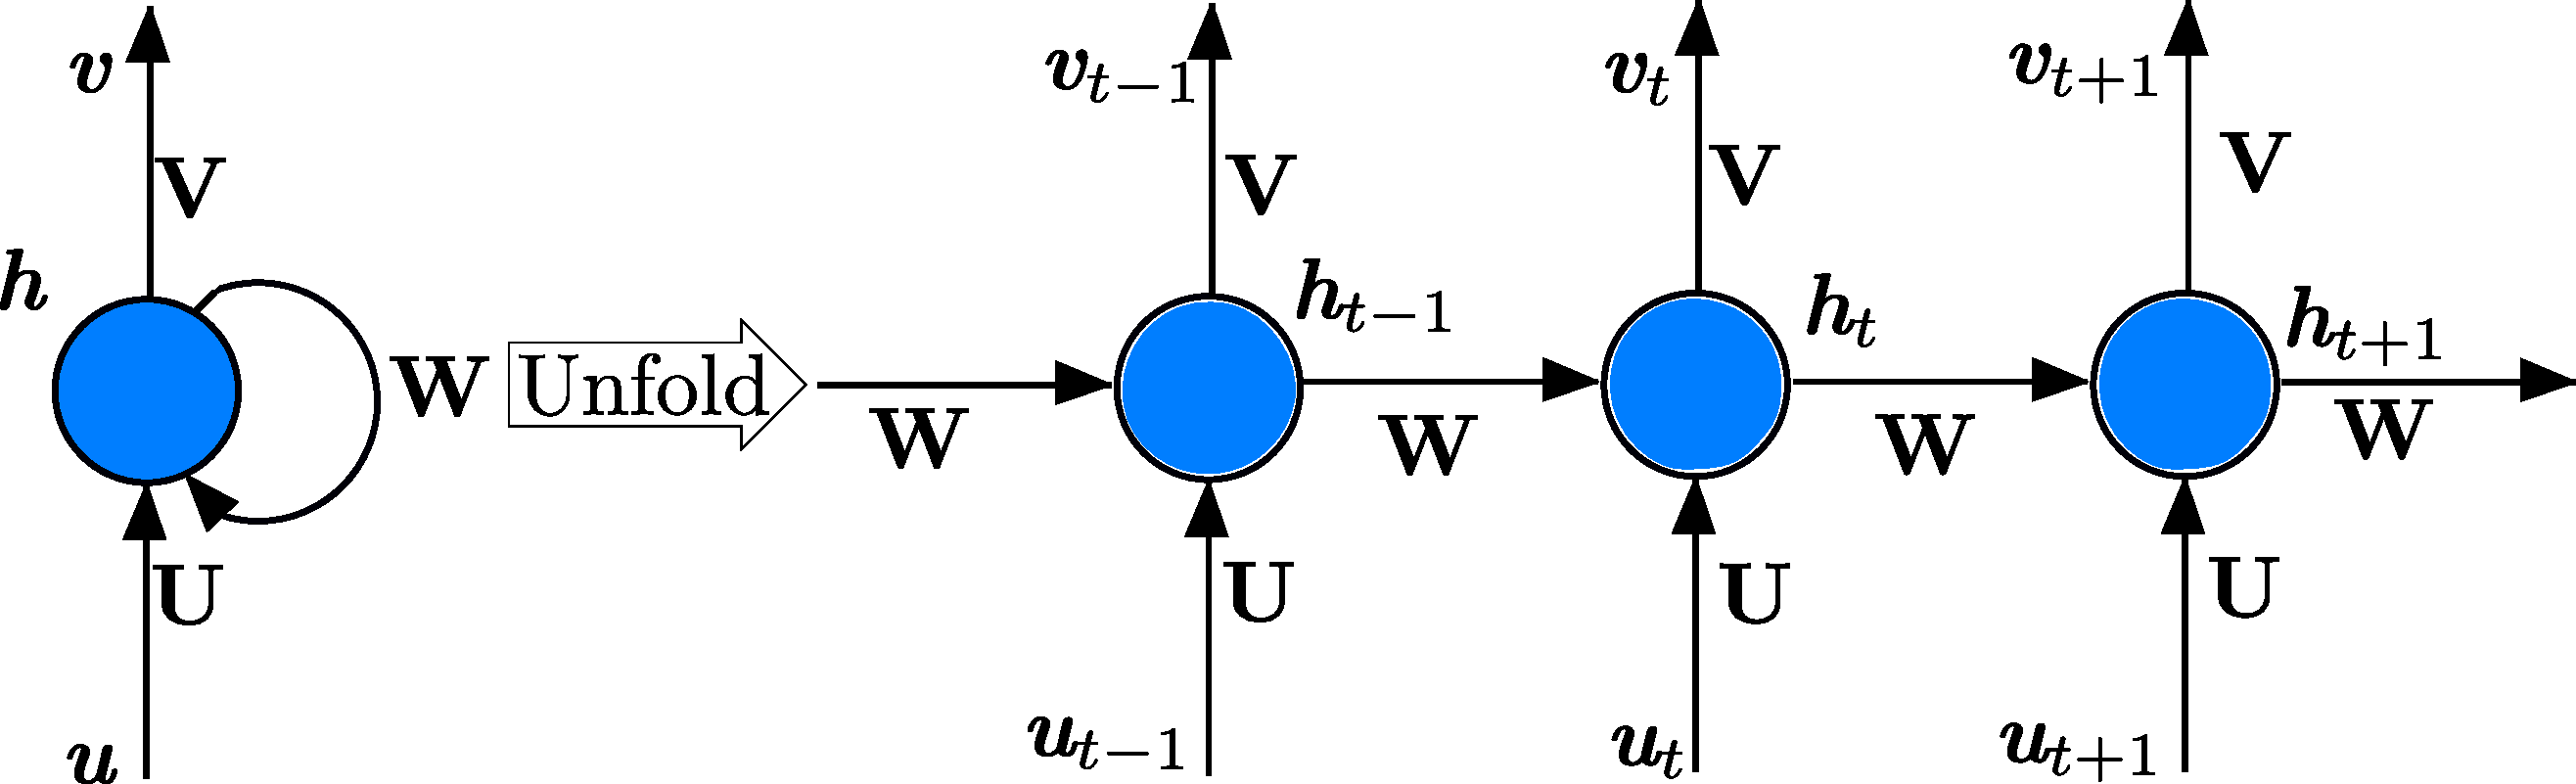
\includegraphics[width=\textwidth]{RNN}
		\caption{}
	\end{subfigure}
	\caption{Typical representation of an RNN. The weight matrices $ \textbf{U} $, $ \textbf{V} $ and $ \textbf{W} $ operate linearly on the input vector $ \textbf{u} $, output vector $ \textbf{v} $ and the internal state variables $ \textbf{h} $, respectively. The hidden state is passed along the input series.}\label{fig-nn-rnn}
\end{figure}

The problem of vanishing gradient during RNN training with standard gradient-based optimizers\cite{kolenGradientFlowRecurrent2001} delays the training process. To avoid this problem, a specific cell called Long-Short Term Memory (LSTM) can be used\cite{hochreiterLongShortTermMemory1997}. A typical LSTM cell at time $ t $, shown in Figure \ref{fig-nn-lstm}(a), processes the input vector $ \textit{\textbf{u}}_{t} $ along with a set of history vectors made of a hidden state $ \textbf{\textit{h}}_{t-1}\in\mathbb{R}^k $ and the cell state $ \textbf{\textit{C}}_{t-1}\in\mathbb{R}^k $, $ k $ being the size of the LSTM cell. The LSTM cell outputs a vector $ \textbf{\textit{v}}_t $ and updates the history vectors, the hidden state $ \textbf{\textit{h}}_{t} $ and the cell state $ \textbf{\textit{C}}_{t} $. The cell state $ \textit{\textbf{C}}_t $ is like a conveyor belt that undergoes only minor linear interactions to ``forget" information that is not needed to be stored for future purpose. The hidden state $ \textbf{\textit{h}}_t $ is nothing but the output of the cell that is used to influence the behavior of the cell at time $ t+1 .$A 1D cyclic loading based elasto-visco-plastic material study has been described in \cite{ghavamianAcceleratingMultiscaleFinite2019} using LSTMs and theoretically the applicability to a 2D loading case should not be unrealistic provided that 
%TODO Ensure not in next page with \enlargethispage{\baselineskip}
the structure is properly designed and trained.
\enlargethispage{\baselineskip}

\begin{figure}
	\centering
	\begin{subfigure}[t]{0.51\textwidth}
		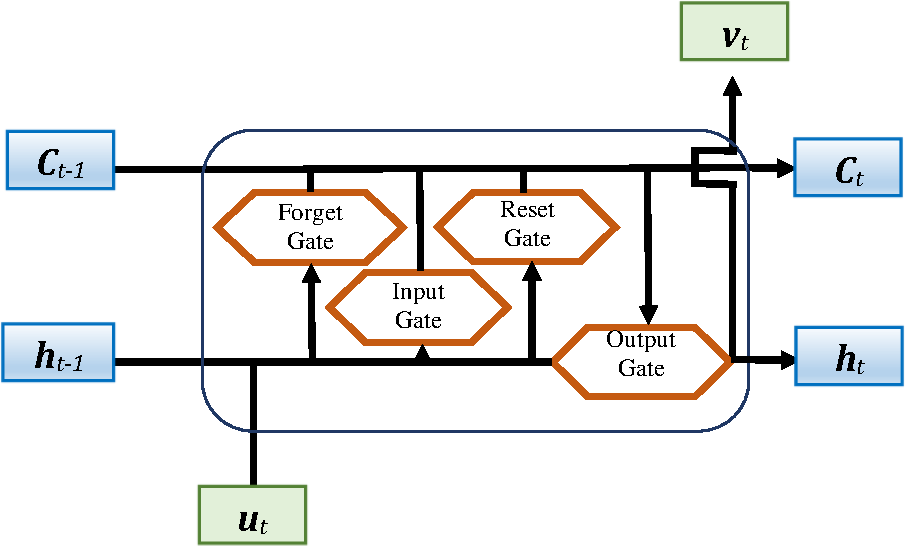
\includegraphics[width=\textwidth]{LSTM_base}
		\caption{}
	\end{subfigure}
	\begin{subfigure}[t]{0.45\textwidth}
		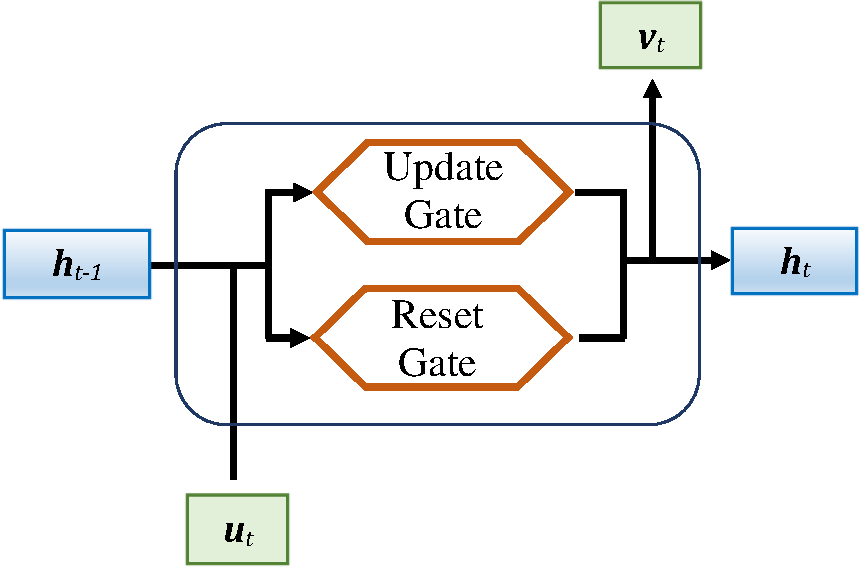
\includegraphics[width=\textwidth]{GRU_base}
		\caption{}
	\end{subfigure}
	\caption{(a) A long-short term memory module (LSTM) with cell state $ \textit{\textbf{C}} $, hidden state $ \textbf{\textit{h}} $, input vector $ \textbf{\textit{u}} $ and output vector $ \textbf{\textit{v}} $. (b) A gated recurrent unit (GRU) where the cell state and hidden states are merged, and the forget gate and the input gate of the LSTM cell have been replaced by an update gate.}\label{fig-nn-lstm}
\end{figure}

A Gated Recurrent Unit (GRU) is a slightly modified LSTM cell\cite{choLearningPhraseRepresentations2014}. A reset and an update gate control the amount of information to be activated and passed to the next node. The feedback loops can be used in these cells to control the stored states of the cells, and this is the reason such networks can be called Feedback Neural Networks. In \cite{wuRecurrentNeuralNetworkaccelerated2020}, a GRU based network is coupled with two feed forward NNWs at the inner layer and the outer layer to study the implementation of an RNN as a surrogate of the micro-scale BVP in the context of computational multi-scale analyses. 

In this work, RNN models based on LSTM and GRU cells will be used to study the training, validating and testing of ANN as surrogates for micro-scale BVP when the loading pattern history dependency is involved. The internal architecture of these RNN cells are presented in Appendix \ref{app-lstm}.

\subsection{Double Feed forward Networks (\fnn)}\label{nn-fnn2}
In traditional \fee-methods, the state of the micro-structure during the micro-scale BVP resolution is used to obtain the averaging of the stress tensors based on the boundary conditions formulated from the strain tensors, and necessary to compute the macroscopic response as explained in Chapter \ref{chap-ch}. This can be termed analogous to the cell state of the RNN component cells that constitute the RNNs. In \cite{furukawaImplicitConstitutiveModelling1998}, a state-space based representation of the material model applied on viscoplastic behavior is trained with neural networks made of FNNs. In this work, the methodology will be extended into general elasto-plastic materials, following the work presented by Nguyen et al\cite{nguyenSurrogateModelsBasedUnderPreparation}.

The traditional RNN based networks will be studied and compared to this double FNN based network, that will be called as \fnn. In this the state of the neural network will be replaced by the state snapshot of the material model at each time step that effectively represents the complete behavior of the material without needing to resort to historical information. Two FNNs will be used to train, validate and test the incremental behavior of the history dependent material model and its performance will be analyzed.

Figure \ref{fig-nn-fnn2} illustrates the \fnn model that is proposed. A state-space representation based variable is provided as an additional input to the network combination in a treatment similar to what an RNN module does. The first part of the \fnn network outputs the incremental state variable which is then used as an input to the second half of the network to get the final output, or this incremental state variable can be used in a standard FEM analysis to predict the behavior of the material using a standard iterative solver.

\begin{figure}
	\centering
	\begin{subfigure}[t]{0.45\textwidth}
		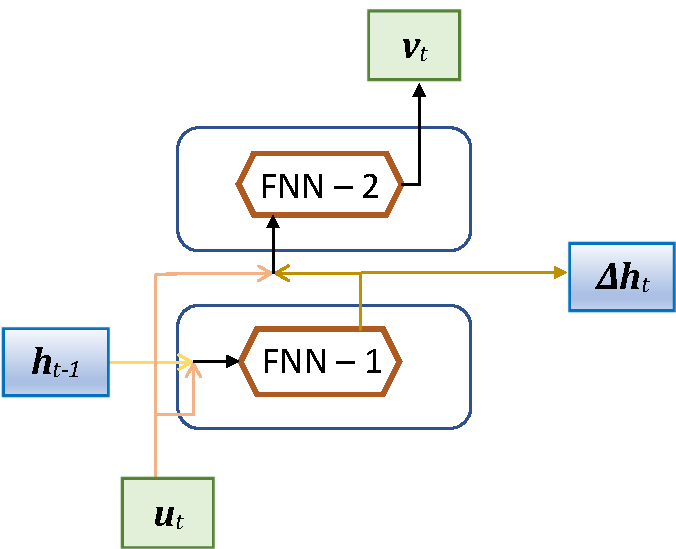
\includegraphics[width=\textwidth]{FNN2}
	\end{subfigure}
	\caption{A double FNN based \fnn neural network model with input vector $ \textbf{\textit{u}} $, the output vector $ \textbf{\textit{v}} $ and the state variables $ \textbf{\textit{h}} $. The incremental state variables $ \bm\Delta\textbf{\textit{h}}_t $ is passed from the first network to the second network and can be extracted in between to be used in a standard FEM based simulation.}\label{fig-nn-fnn2}
\end{figure}

\subsection{Comparison of the architectures}\label{nn-compare}
Two approaches to study history dependent behavior, so called RNN-based and \fnn-based, have been summarized in the previous subsections. Some notable differences between the two approaches are as follows:
\begin{itemize}
	\item The inputs of the RNN models need to be arranged in a sequential manner so that the time-based series can update the hidden pattern that might exist underlying in the series. However, only the current and the successive state values are necessary for the \fnn models.
	\item The constituent cell states in RNNs are automatically updated during the training process and need no external manipulations from the user. For \fnn models, the user has to choose the respective material parameters depending on the type of training the \fnn is used for. These \textit{a priori} parameters, like plastic strain, etc, would then best represent the behavior of the material.
\end{itemize}
In the following sections, the comparison in terms of the performance of the respective models will also be outlined.

\section{Generation of Datasets for ANNs}\label{nn-gendata}
In order to train an ANN that can be used as a surrogate for the micro-scale behavior in the standard multi-scale computational homogenization procedure outlined in Chapter \ref{chap-ch}, it is imperative to choose the appropriate input and output parameters in Eq. (\ref{eq-nn-func}). It is obvious that one has to use the same input parameters that are used in the micro-scale BVP described by Eq. (\ref{eq-micro-3-1}) so that the ANN can be trained to predict the output of the BVP problem. 

\subsection{Geometry Description for ANN study}\label{app-geom}
The 3D open-foam FE models generated based on the tools explained in the Chapter \ref{chap-of} are very expensive. Indeed, the downside of an explicit geometry is the high number of elements in the discretized model. In order to simplify the study and to obtain a better understanding of the impact and usefulness of the data driven models, a simplified two dimensional version of the open foam model will be used in the following sections to develop a training strategy. Based on Eq. (\ref{voronoi}), a two dimensional tessellation of a circular inclusion packing is developed and following the mesh refinement strategy proposed in Section \ref{of-fem}, a finite element discretization is generated. The model consists of approximately 16 circular inclusions tessellated in a unit square domain to generate an FEM representation that is not periodic in structure. The final mesh has around 2000 triangular elements (Figure \ref{fig-nn-model}).
%A simpler model was also developed that consists of an X-shaped structure with introduced irregularities to help develop early data driven solvers (Figure \ref{fig-nn-model}b). This simpler model consists of around 250 triangular elements after an FE discretization. 

The developed geometries were analyzed using the multi-scale framework developed in Chapter \ref{chap-ch}. The material properties and the material model used in Section \ref{res-fem} are also considered here.

\begin{figure}
	\centering
	\begin{subfigure}[t]{0.45\textwidth}
		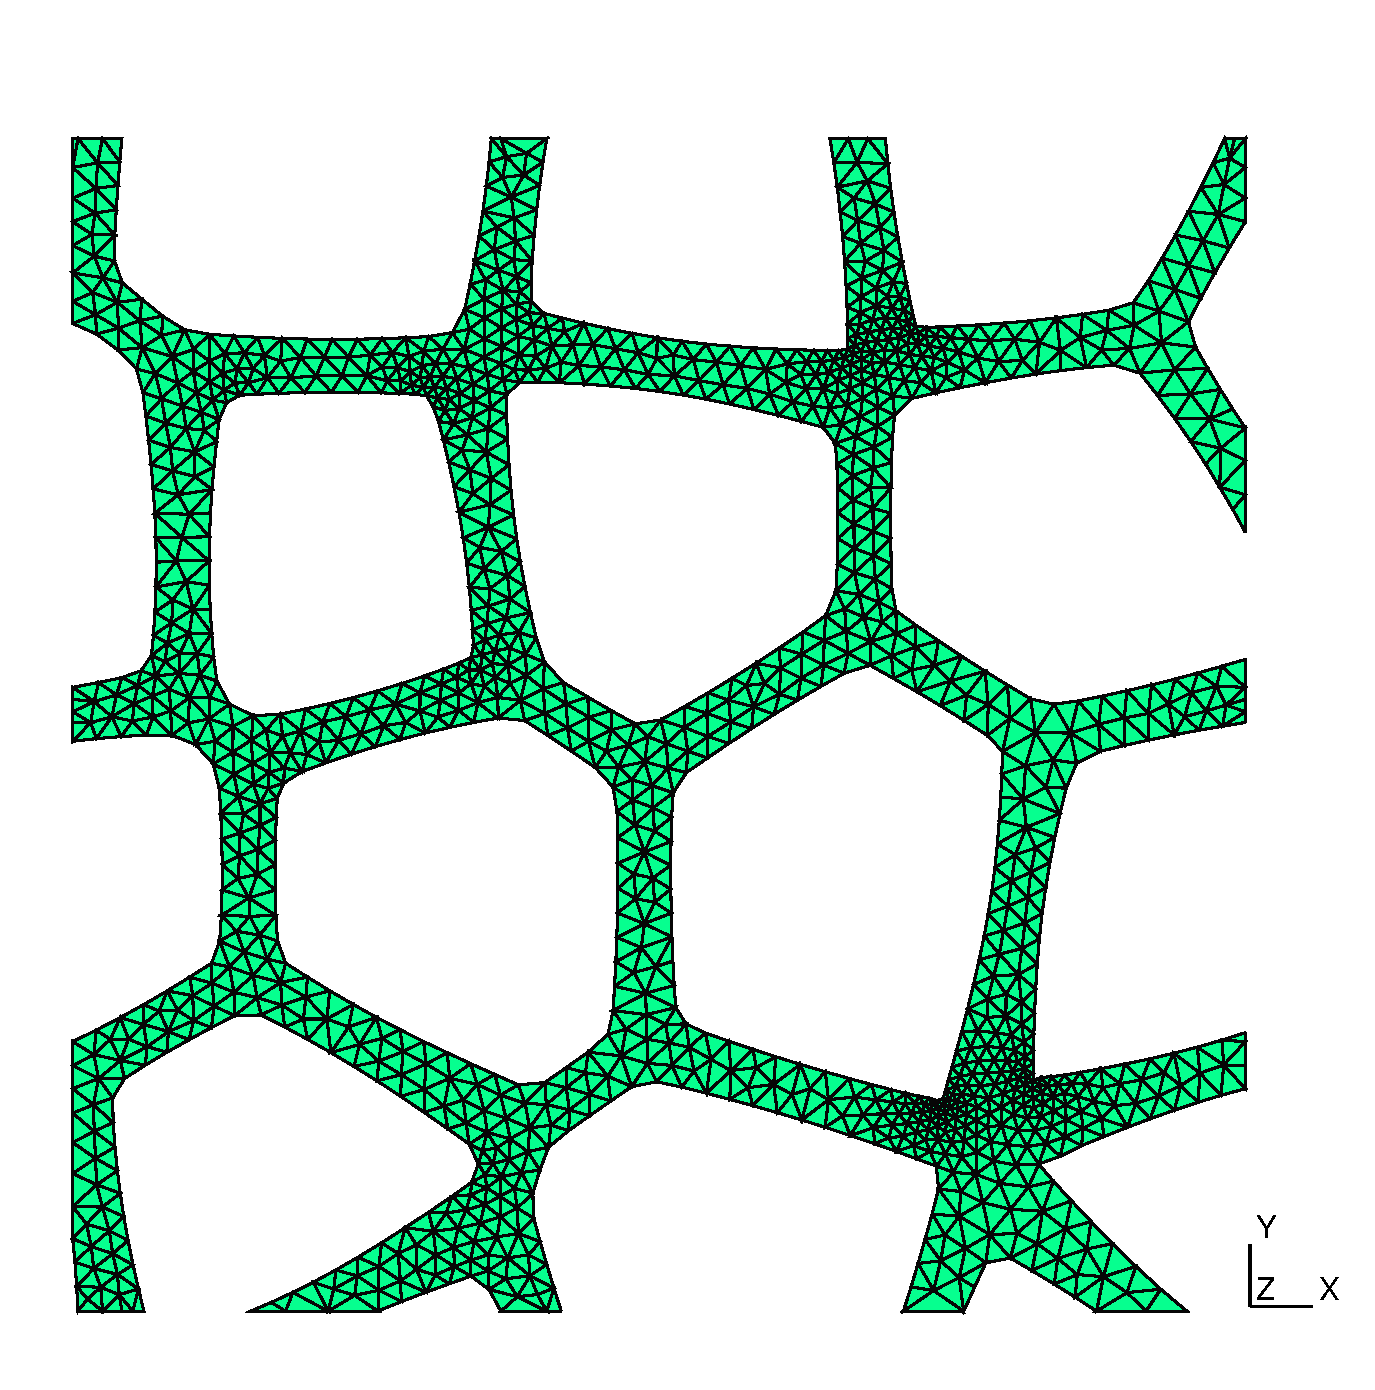
\includegraphics[width=\textwidth]{2d_foam}
		\caption{}
	\end{subfigure}
%	\begin{subfigure}[t]{0.45\textwidth}
%		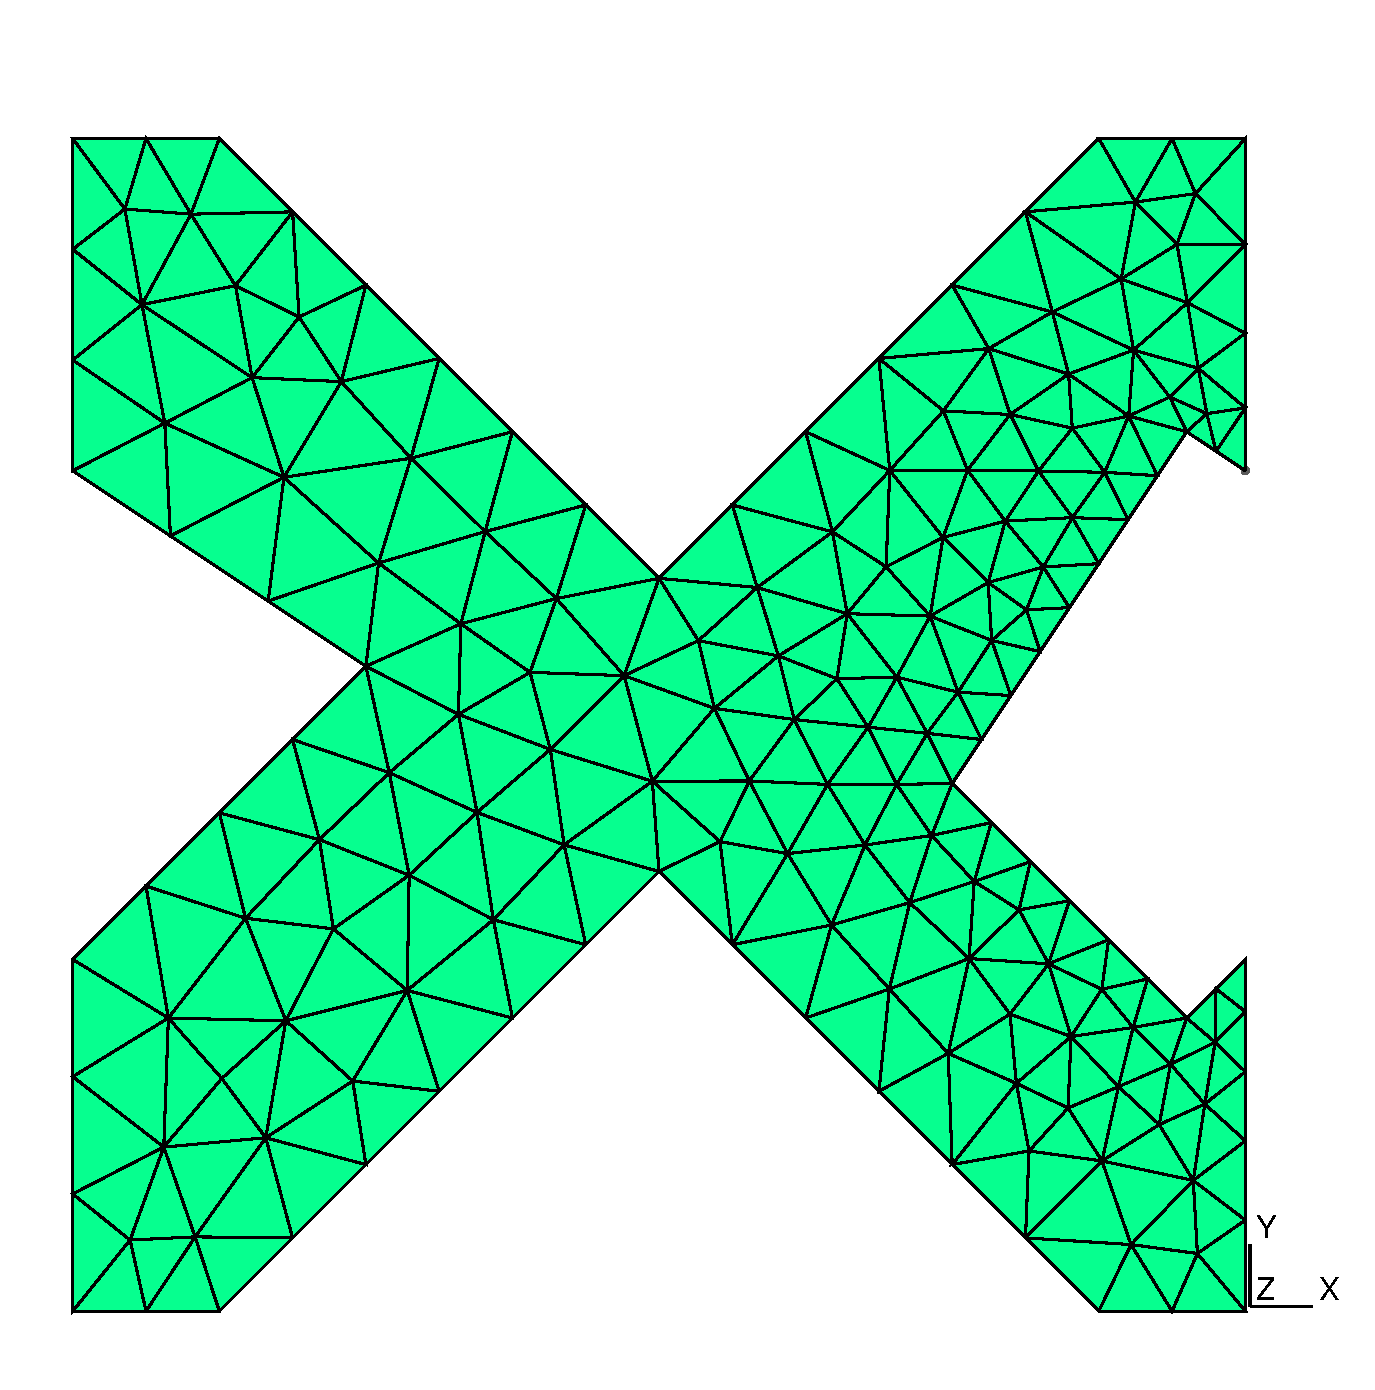
\includegraphics[width=\textwidth]{2d_simple}
%		\caption{}
%	\end{subfigure}
	\caption{A 2D simplification of an open foam geometry consisting of around 2000 triangular elements.
%		; and (b) A 2D simple geometry with around 250 triangular elements
	}\label{fig-nn-model}
\end{figure}


\subsection{Description of the micro-scale BVP}\label{nn-bvp}
Considering that the micro-scale BVP presented in Chapter \ref{chap-ch} respects frame indifference, the Green-Lagrangian strain tensor $ \tgm[]{E} $ and the 2$ ^\text{nd} $ Piola-Kirchhoff stress tensor $ \tgm[]{S} $ negates the necessity of accounting for the rigid rotation mode. By describing the stress-strain relationship by $ \tgm[]{E} $ and $ \tgm[]{S} $, the plane strain condition system can be reduced to the input $ \textbf{\textit{u}}=\{E_{\text{M}_{XX}},E_{\text{M}_{YY}},E_{\text{M}_{XY}}\} $ with the output as $ \textbf{\textit{v}}=\{S_{\text{M}_{XX}},S_{\text{M}_{YY}},S_{\text{M}_{ZZ}},S_{\text{M}_{XY}}\} $. Consequently it becomes important to obtain the required input values $ \tgm[]{E} $ from $ \tgm[]{F} $ to train the ANN and also to obtain $ \tgm[]{S} $ from $ \tgm[]{P} $ to subsequently feed into the macro-scale analysis, simply by
\begin{equation}\label{eq-nn-io}
\tgm[]{E} = \frac{1}{2}\left(\tgm[]{F}^T\cdot\tgm[]{F}-\textbf{I}\right),
\end{equation}
and
\begin{equation}\label{eq-nn-io-1}
\tgm[]{S} = \tgm[]{F}^{-1}\cdot\tgm[]{P}.
\end{equation}

For the study of the implementation of micro-scale surrogates using ANNs, the input and output parameters considered here, with individual stress-strain states for FNNs and sequences of stress-strain states of individual training case for RNNs that are suitably generated can be used. However in the case of \fnn, one can use individual stress-strain states along with the internal-states, $ \tgm{Z} $, as the input-output parameters. In this situation, the input at stage $ t $ is $ \textbf{\textit{u}}_t=\{{{{E}}_{XX}}_t,{{{E}}_{YY}}_t,{{{E}}_{XY}}_t,{\tgm{Z}}_{t-1}\} $ while the output is now $ \textbf{\textit{v}}_t=\{{{{S}}_{XX}}_t,{{{S}}_{YY}}_t,{{{S}}_{ZZ}}_t,{{{S}}_{XY}}_t,{\tgm{Z}}_{t}\} $. The generation of these states will be explained in this Section.

In the scope of limiting the solution space to a value that can be discretized, it becomes important that a well defined approach to prepare input data is utilized. Even though $\tgm[]{E} $ is chosen as the input of the ANN, it can not be used directly as the boundary condition in Eq. (\ref{eq-periodic-3}). The connection between $ \tgm[]{F} $ and $ \tgm[]{E} $ can be instead established by the right stretch tensor $ \tgm[]{U} $.  With the assumption that the micro-scale BVP is frame indifferent, the rotational decomposition of $ \tgm[]{F} $
\begin{equation}\label{eq-nn-gen1}
\tgm[]{F}=\tgm[]{R}\cdot\tgm[]{U},
\end{equation}
with the rotation tensor $ \tgm[]{R}=\textbf{I} $ as it can be arbitrarily chosen. 

To facilitate the macro-scale simulation, the necessary material parameter tensor in the macro-scale, $ \mathbb{C}_\text{M} $ can be simply obtained as $ \partial\tgm[]{S}/\partial\tgm[]{E} $ using the implicit based differentiation functions available in the standard repositories used to train the models.

\subsection{Proportional loading}\label{nn-gendata-prop}
In the case of monotonic loading, the loading strain can be divided into the proportional components in the component axis. As a symmetric second order tensor, a spectral decomposition can be applied to the right stretch tensor so as to obtain the form
\begin{equation}\label{eq-nn-gen2}
\tgm[]{U}=\lambda_1\textbf{n}_1\otimes\textbf{n}_1+\lambda_2\textbf{n}_2\otimes\textbf{n}_2+\lambda_3\textbf{n}_3\otimes\textbf{n}_3,
\end{equation}
with eigenvalues $ \lambda_i $ and eigenvectors $ \textbf{n}_i $ where $ i={1,2,3} $, controlling the loading and the direction of the loading respectively. With the help of an orthogonal vector and eigenvalue generator, it is possible to reclaim the strain space that covers the entire domain of monotonic loading. The three eigenvalues can be generated to satisfy the condition
\begin{equation}\label{eq-nn-gen3}
\sqrt{\lambda_1^2+\lambda_2^2+\lambda_3^2}\le R_\text{max},
\end{equation}
where $ R_\text{max} $ is a fixed upper bound. $ \Delta\tgm[]{U} $ which is the incremental strain can be chosen such that the minimum possible strain increment is captured to ensure the availability of all possible strain space.

A set of variables $ u_i\in\mathbb{R} $, $ i=1,2,3 $ that are realizations of a Gaussian distribution $ \mathcal{N}(0,1) $, can be used to generate a uniform distribution of the strain space $ \tgm[]{U} $\cite{NoteMethodGenerating}, with
\begin{equation}\label{eq-nn-gen7}
\lambda_1=\frac{u_1R}{\sqrt{u_1^2+u_2^2+u_3^2}},
\end{equation}
\begin{equation}\label{eq-nn-gen7-1}
\lambda_2=\frac{u_2R}{\sqrt{u_1^2+u_2^2+u_3^2}},
\end{equation}
and
\begin{equation}\label{eq-nn-gen7-2}
\lambda_3=\frac{u_3R}{\sqrt{u_1^2+u_2^2+u_3^2}},
\end{equation}
with
\begin{equation*}
%u_1\sim\mathcal{N}(0,1),\quad u_2\sim\mathcal{N}(0,1),\quad u_3\sim\mathcal{N}(0,1)\ \ \text{and}\ \
\left(u_1^2+u_2^2+u_3^2\right)\ne0,
\end{equation*}
and $ R\le R_\text{max} $
This distribution ensures that as many random strain states as possible are covered and that the strain points are not cluttered at the poles of the strain sphere.

Keeping in mind a 2D plane-strain case, $  \textbf{n}_3 $ can be fixed. Generally, a uniformly distributed angular random variable with realization $ \alpha\in\left[ 0,\pi \right) $ can be used to generate the set of random orthogonal vectors $ \textbf{n}_1 $ and $ \textbf{n}_2 $, by
\begin{eqnarray}\label{eq-nn-gen4}
\textbf{n}_1=
\begin{bmatrix}
\cos\alpha \\
\sin\alpha
\end{bmatrix}
& \text{and} & \textbf{n}_2=
\begin{bmatrix}
-\sin\alpha\\
\cos\alpha
\end{bmatrix}.
\end{eqnarray} 
An approach to obtain the parameterized values of the loading tensor is further explained in Appendix \ref{app-angle} for a symmetric matrix and can be applied here for a 2D case.

\subsubsection{Proportional monotonic loading}\label{nn-gendata-propdata}
For monotonic behavior, it is assumed that there is only one possible stress-strain relationship for every strain-space. In such situations, a proportional loading path can be used to understand the behavior of material response to the applied strain load. The method to obtain a proportional loading path can be used to obtain the material response for the applied strains in the form of stress tensors. For the training of the output of the ANN, the response of the material law has to be computed for each strain configuration, and this process needs to be done thousands of times to generate as many stress-strain states $ \left[\tgm[]{E},\tgm[]{S}\right] $ as possible to be trained. There is a good chance that the simulation will not converge in a given $ \Delta\tgm[]{U} $ increment and in such cases the increment size needs to be reduced to continue the convergence path. In the present scenario, the reduction of this increment size has been kept to a minimum possible number of times so as to ensure that the increment step does not become too small. It is also possible in such situations the simulation fails. The data obtained from such a failed simulation is still utilized in the training sequence until the strain step of failure.

This process can be summarized as follows:
\begin{itemize}
	\item Select $ \lambda_1 $ and $ \lambda_2 $ as given in Eqs. (\ref{eq-nn-gen7}) and (\ref{eq-nn-gen7-1});
	\item Select a uniformly distributed angular random variable with realization $ \alpha\in\left[0,\pi\right) $;
	\item Compute $ \tgm[]{U} $ according to Eq. (\ref{eq-nn-gen2});
	\item Arrange $ \tgm[]{U}=\left[..,{\tgm[]{U}}_{i-1},{\tgm[]{U}}_{i},{\tgm[]{U}}_{i+1},..\right]$ with $ i=\left[0,...,N_S\right] $ so that ${\tgm[]{U}}_{i}={\tgm[]{U}}_{i-1}+\Delta{\tgm[]{U}}_i $ and where $ {\tgm[]{U}}_0=\textbf{I} $ is the first step.
\end{itemize}

\subsubsection{Proportional cyclic loading}\label{nn-gendata-cycdata}
Proportional loading can also be used to record history dependent behavior in materials by reversing the direction of the load after plasticity is achieved. The stress-strain states are no more unique and therefore standard FNNs can no more be used in this scenario and one needs to train these states with either RNNs or \fnn. The load reversal can be obtained by using $ \alpha = \pi-\alpha $ that results in the orthogonal vectors having an inverse direction.

This process can be summarized as follows:
\begin{itemize}
	\item Complete all the steps from Section \ref{nn-gendata-propdata} and obtain $ \lambda_1 $, $ \lambda_2 $ and $ \alpha $;
	\item Select angular random variable $ \pi-\alpha $ and compute $ \tgm[]{U} $ according to Eq. (\ref{eq-nn-gen2});
	\item Arrange $ \tgm[]{U}=\left[{\tgm[]{U}}_0,...,{\tgm[]{U}}_{i},...,{\tgm{U}}_{2N_S}\right]$ with $ i=\left[0,...,2N_S\right] $ where $ {\tgm[]{U}}_0=\textbf{I} $ is the first step and $ {\tgm[]{U}}_{2N_S}=\textbf{I} $ is the last step.
\end{itemize}

\subsection{Random path loading for history dependent behavior}\label{nn-gendata-rand}
History dependent behavior, like non-proportional cyclic loading in materials, is a complex process that involves a lot of local plasticity and strain concentration. Even in the case of proportional loading, it is not possible to account for local plasticity occurring at various points in a complex micro-structure. In order to capture the entire stress-strain space that is possible in a history dependent process, one has to discretize the regular grid into really small portions which might not be computationally feasible. In \cite{wuRecurrentNeuralNetworkaccelerated2020}, random combination of the loading strain sequenced into a format called random path has been found very effective in capturing a statistical representation of the strain space that could be generated by a material deforming under a hysteresis like behavior. Series of such random loading paths, which can be considered as a random walk in a stochastic process, is necessary to be generated in a sequential manner to train the RNNs.

By definition, for a random path generation, $ \Delta{\tgm[]{U}}_n={\tgm[]{U}}_n-{\tgm[]{U}}_{n-1} $ is a random vector that allows the loading path to have variable direction at each step. This way, one can ensure that a maximum number of non-proportional loading conditions can be covered.
Analogous to Eq. (\ref{eq-nn-gen2}), a spectral decomposition of the increment of the right stretch tensor gives
\begin{equation}\label{eq-nn-gen5}
\Delta\tgm[]{U}=\Delta\lambda_1\textbf{n}_1\otimes\textbf{n}_1+\Delta\lambda_2\textbf{n}_2\otimes\textbf{n}_2+\Delta\lambda_3\textbf{n}_3\otimes\textbf{n}_3
\end{equation}
where $ \Delta\lambda_i\ i=1,2,3 $, control the increment size. Similar to Eq. (\ref{eq-nn-gen3}), the three eigenvalues can be generated as
\begin{equation}\label{eq-nn-gen6}
\sqrt{\Delta\lambda_1^2+\Delta\lambda_2^2+\Delta\lambda_3^2}\le \Delta R.
\end{equation}
Considering the 2D case, similar to Eqs. (\ref{eq-nn-gen7}) and (\ref{eq-nn-gen7-1}), $ \Delta\lambda_1^2 $ and $ \Delta\lambda_2^2 $ can be generated by the random split of a random variable with an allowable maxima and minima to avoid really small steps from cluttering the training. Following Eq. (\ref{eq-nn-gen4}), random orthogonal vectors, $ \textbf{n}_1 $ and $ \textbf{n}_2 $, can be generated to obtain a random loading direction.

A stopping criterion becomes necessary considering that the random walk can go on until there is a limit. This can be achieved by using a global $ R_\text{max} $ as a critical value, with the random walk generator stopped when yielding the criterion $ \sqrt{\sum_{i=1}^3\left(\lambda_i-1\right)^2}>R_\text{max} $ is reached, or a limit on the total number of steps the random walk generator can undergo, or a combination of the two, to obtain in the format
\begin{equation}\label{eq-nn-path}
\tgm[]{U}^i=\left[{\tgm[]{U}^i}_0,{\tgm[]{U}^i}_1,{\tgm[]{U}^i}_2,...,{\tgm[]{U}^i}_{N_S}\right]
\end{equation}
with $ {\tgm[]{U}}^i_0 =\textbf{I}$ as the starting value of the paths and $ N_S $ being the number of steps in the sequence.

%\subsection{Random path loading }\label{nn-gendata-randpath}
Generally, RNNs expect sequential training dataset from which these units can then understand the historical statistical relations. Because of this, it becomes a necessity to obtain the training data in a sequential format as the RNNs accept inputs in long sequences. The loading path generated is bound between a maximum and a minimum, and within this range is allowed to propagate in any manner that the randomly generated increment so chooses.

The algorithm for the random path generation can be summarized as follows:
\begin{enumerate}
	\item Choose $ {\tgm[]{U}}_0=\textbf{I} $ for $ i=0 $ as the starting step;
	\item Following the angle based parametrization presented in Appendix \ref{app-angle}, select three independent random variables uniformly distributed with realizations $ \alpha\in\left[0,\pi\right) $ that give the random loading direction, $ \varphi\in\left[0,2\pi\right) $ and $ \mathcal{R}\in\left(\Delta R^2_\text{min},\Delta R^2\right] $, together yielding $ \Delta\lambda_1=\sqrt\mathcal{R}\cos(\varphi) $, and $ \Delta\lambda_2=\sqrt\mathcal{R}\sin(\varphi) $, with $ \Delta R_\text{min} $ representing a minimum bound to avoid too small a step, and $ \textbf{n}_1 $, $ \textbf{n}_2 $ following Eq. (\ref{eq-nn-gen4});
	\item The incremental strain can be computed on the basis of the angle based paramterization as $ \Delta{\tgm[]{U}}_{k+1}$ following Eq. \ref{eq-nn-gen5};
	\item If $ ||{\tgm[]{U}}_k+\Delta{\tgm[]{U}}_{k+1}-\textbf{I}||<R_\text{max} $ update the strain value $ {\tgm[]{U}}_k $ with the computed $ \Delta{\tgm[]{U}}_{k+1} $, so that $ {\tgm[]{U}}_{k+1}={\tgm[]{U}}_k+\Delta{\tgm[]{U}}_{k+1} $ else go back to step 2;
	\item If $ i<N_S $, update $ i=i+1 $ and go to step 2, else terminate the random walk algorithm.
\end{enumerate}

%In cases of complex models with large behavioral ranges for constitutive loading, the amount of data generated, or that needs to be trained can be quite humongous and the models might end up inefficient in their predictive capabilities. In the beginning of training to test models and to understand the behavior of RNNs, it was decided to test the models for discrete jumps in the strain values rather than a range of continuous values. In this regard, the strain sequences can be visualized as a network of paths that were built with an octant basis and was allowed to reach the target strain path in a closest possible way without having to sacrifice on the randomness of the path.

%In the case of 2D plane strain, one can ensure this, by introducing minimum constant strain jump $ [\Delta{\tgm[]{U}}_{XX},\Delta{\tgm[]{U}}_{YY}\Delta{\tgm[]{U}}_{XY}] $ that defines the sides of the first octant. By considering the Euclidean distance between the target strain $ {\tgm[]{U}}_{k+1} $ from all the octant nodes of $ {\tgm[]{U}}_k $, one can determine the shortest discrete path to reach the target strain. Figure \ref{fig-nn-quadrant} displays this  analogy in 2D space on a quadrant. The nearest point in the quadrant to the target point $ x_{k+1} $, denoted by $ x_{k+1}' $ is the final point chosen by the algorithm.

It is interesting to note here that the random path loading can also be used to generate a pseudo random proportional loading scenario where the randomness is confined to a single walking direction, and is restricted at a certain maximum.

%\begin{figure}
%	\centering
%	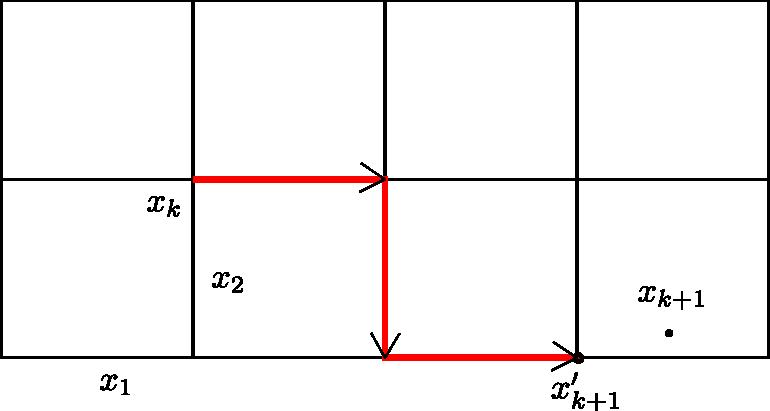
\includegraphics[height=5cm]{quadrant_progress}
%	\caption{Quadrant approach to find the closest path in a discrete space between two points $ x_k $ and $ x_{k+1} $.}\label{fig-nn-quadrant}
%\end{figure}

\subsection{State-based Representation}\label{nn-dnn-state}
In the context of history-dependent processes, like the one represented by Eq. (\ref{eq-dG-bilinear}), it is useful to represent the system with the help of an internal state representation vector, $ \textbf{Z} $\cite{rezguiPredictiveElastoplasticDamage2016}. A similar approach has been tackled in \cite{furukawaImplicitConstitutiveModelling1998} with the introduction of the state-space method and the description of the material behavior without any phenomenological formulations by constructing it based only on the experimental data. This approach has been extended to the storage of the internal state representation vector extracted from the response to deformation gradients of the material law in FEM formulations. The purpose of this vector is to gather all the internal variables (plasticity, damage, etc) that describe the irreversible phenomena. At the homogeneous level, at any given point of time $ t $, this can be represented as
\begin{equation}\label{eq-ch-state1}
\tgm[]{P}(t)=\mathcal{P}_M(\tgm[]{F}(t);\tgm[]{Z}(t)).
\end{equation}
This coupled representation provides a complete snapshot of the state of the system while following the underlying constitutive laws. Also, this representation assumes that the evolution laws of the internal variables $ \tgm[]{Z} $ follow the rate form
\begin{equation}\label{eq-ch-state2}
\overset{.}{\textbf{Z}}_\text{M}(t)=\mathcal{Z}_M(\tgm[]{Z}(t),\tgm[]{U}(t),\overset{.}{\textbf{U}}_\text{M}(t))
\end{equation}
where $ \tgm[]{U}=\sqrt{\tgm[]{C}}=\sqrt{\tgm[]{F}^T\cdot\tgm[]{F}} $ is the right stretch tensor. $ \tgm[]{U} $ is assumed to be frame invariant which leads to the assumption that $ \tgm[]{Z}$ is also frame invariant. $  \tgm[]{U} $ can be directly used to define the microscopic boundary condition and thus is advantageous as the lead kinematic variable in a lot of cases. The state-based representation of a history-dependent constitutive law is completed by
\begin{equation}\label{eq-ch-state3}
\tgm[]{S}(t)=\mathcal{S}_M(\tgm[]{U}(t),\tgm[]{Z}(t))
\end{equation}
where the  $ 2^\text{nd} $-Piola Kirchhoff tensor $ \tgm[]{S} $ is chosen at the macro-scale because of its frame invariant nature. 

With the RVE consisting of multiple constituents $ \alpha=1,...,N_{pm} $ with $ N_{pm} $ number of constituents, each constituent $ \alpha $ has its mechanical behavior explicitly modeled from Eqs. (\ref{eq-ch-state1}) and (\ref{eq-ch-state2}) as
\begin{eqnarray}\label{eq-ch-state4}
\tgmm[]{S}(t) & = & \mathcal{S}^\alpha(\tgmm[]{U}(t),\tgmm[]{Z}(t))\ \ \text{and} \nonumber\\
\overset{.}{\textbf{Z}}_\text{m}(t) & = & \mathcal{Z}^\alpha(\tgmm[]{Z}(t),\tgmm[]{U}(t),\overset{.}{\textbf{U}}_\text{m}(t)). 
\end{eqnarray}
This system needs to be evaluated at each integration point $ \tgmm[]{x}\in\omega $ resulting in internal state variable denoted by $ \tgmm[]{Z}(\tgmm[]{x},t) $ for each integration point. With these points discretized with the focus on a finite element method (FEM), the internal state $ \tgm[]{Z} $ can be represented as
\begin{equation}\label{eq-ch-state5}
\tgm[]{Z}=\{{\tgmm[]{Z}}_i=\mathcal{Z}^\alpha({\tgmm{x}}_i)\ \ \text{for}\ i=1,...,N_{gp}\ \ {\tgmm{x}}_i\in\omega^\alpha\},
\end{equation}
with the integration Gauss points $ N_{gp} $ and internal state $ {\tgmm[]{Z}}_i $ at a given integration point $ i $ in the domain $ \omega^\alpha $ of the constituent $ \alpha $. The various internal state variables that can help in presenting an efficient representation of the model at any given step of an analysis are further explained in Appendix \ref{app-state}.

The variable $ \tgm{Z} $ is a useful indicator for the state of the micro-structure encompassing the entire history of the loading upto that particular point, and is helpful in the study of the \fnn models as a surrogate of the micro-scale computations in the \fee methods.

\subsubsection*{Clustering}\label{nn-dnn-scc}
The state-based representation of the material under study brings in the particular case of increasing number of dimensions that has to be accounted for in an \fnn based surrogate study of complex micro-scale RVEs. The increased number of microscopic state variables becomes a necessity to ensure that the local plasticity is efficiently captured during the training of the ANNs. 

To accelerate the training of the designed ANNs while ensuring a sufficient representation of the material state, the authors in \cite{bessaFrameworkDatadrivenAnalysis2017} present a framework to counter this large ``curse" of large dimensionality. In this section, a similar framework is used to navigate the problem of high dimension number that is faced in the state based representation using a clustering method.

In general, the large number of $ N_{gp} $ in Eq. (\ref{eq-ch-state5}) makes it computationally inefficient to use them effectively in any surrogate based operations and in this regard it is a reduced basis based on domain decomposition or clustering that can be prescribed to describe effectively the internal state over the RVE. An efficient algorithm has been proposed in \cite{liuSelfconsistentClusteringAnalysis2016} using a data compression algorithm called $ k $-means clustering. With the help of a high-fidelity RVE, different points in the material are characterized based on similar mechanical behavior by evaluating their elastic responses and calculating the strain concentration at these points\cite{baiHighfidelityMicroscaleModeling2015}. 

\red{It is assumed that based on the characterization depending on the strain concentration a similarity between two data points can be extracted. The mechanical behavior under any loading condition within the elastic regime is expected to be similar for two such points. Since the localization of plasticity occurs at points of high strain concentrations, the points should also have similar nonlinear plastic response. }

\red{Once the points are characterized, these can be grouped for domain decomposition by using a clustering algorithm called $ k $-means algorithm\cite{macqueenMethodsClassificationAnalysis1967}. The points thus grouped are kept under the same grouping during the extraction of the training data using DNS analysis. Points belonging to the same cluster have approximately same strain concentration and these need not be adjacent (Figure \ref{fig-ch-cluster}). }

\red{This approach has a couple of advantages. In comparison to other clustering approaches like NTFA or POD, one does not need to conduct extensive offline simulations and limits it to the characterization of elastic behavior. Finally, the methodology achieves significant computational gain without forgoing accuracy.}

\begin{figure}
	\centering
	\begin{subfigure}[t]{0.45\textwidth}
		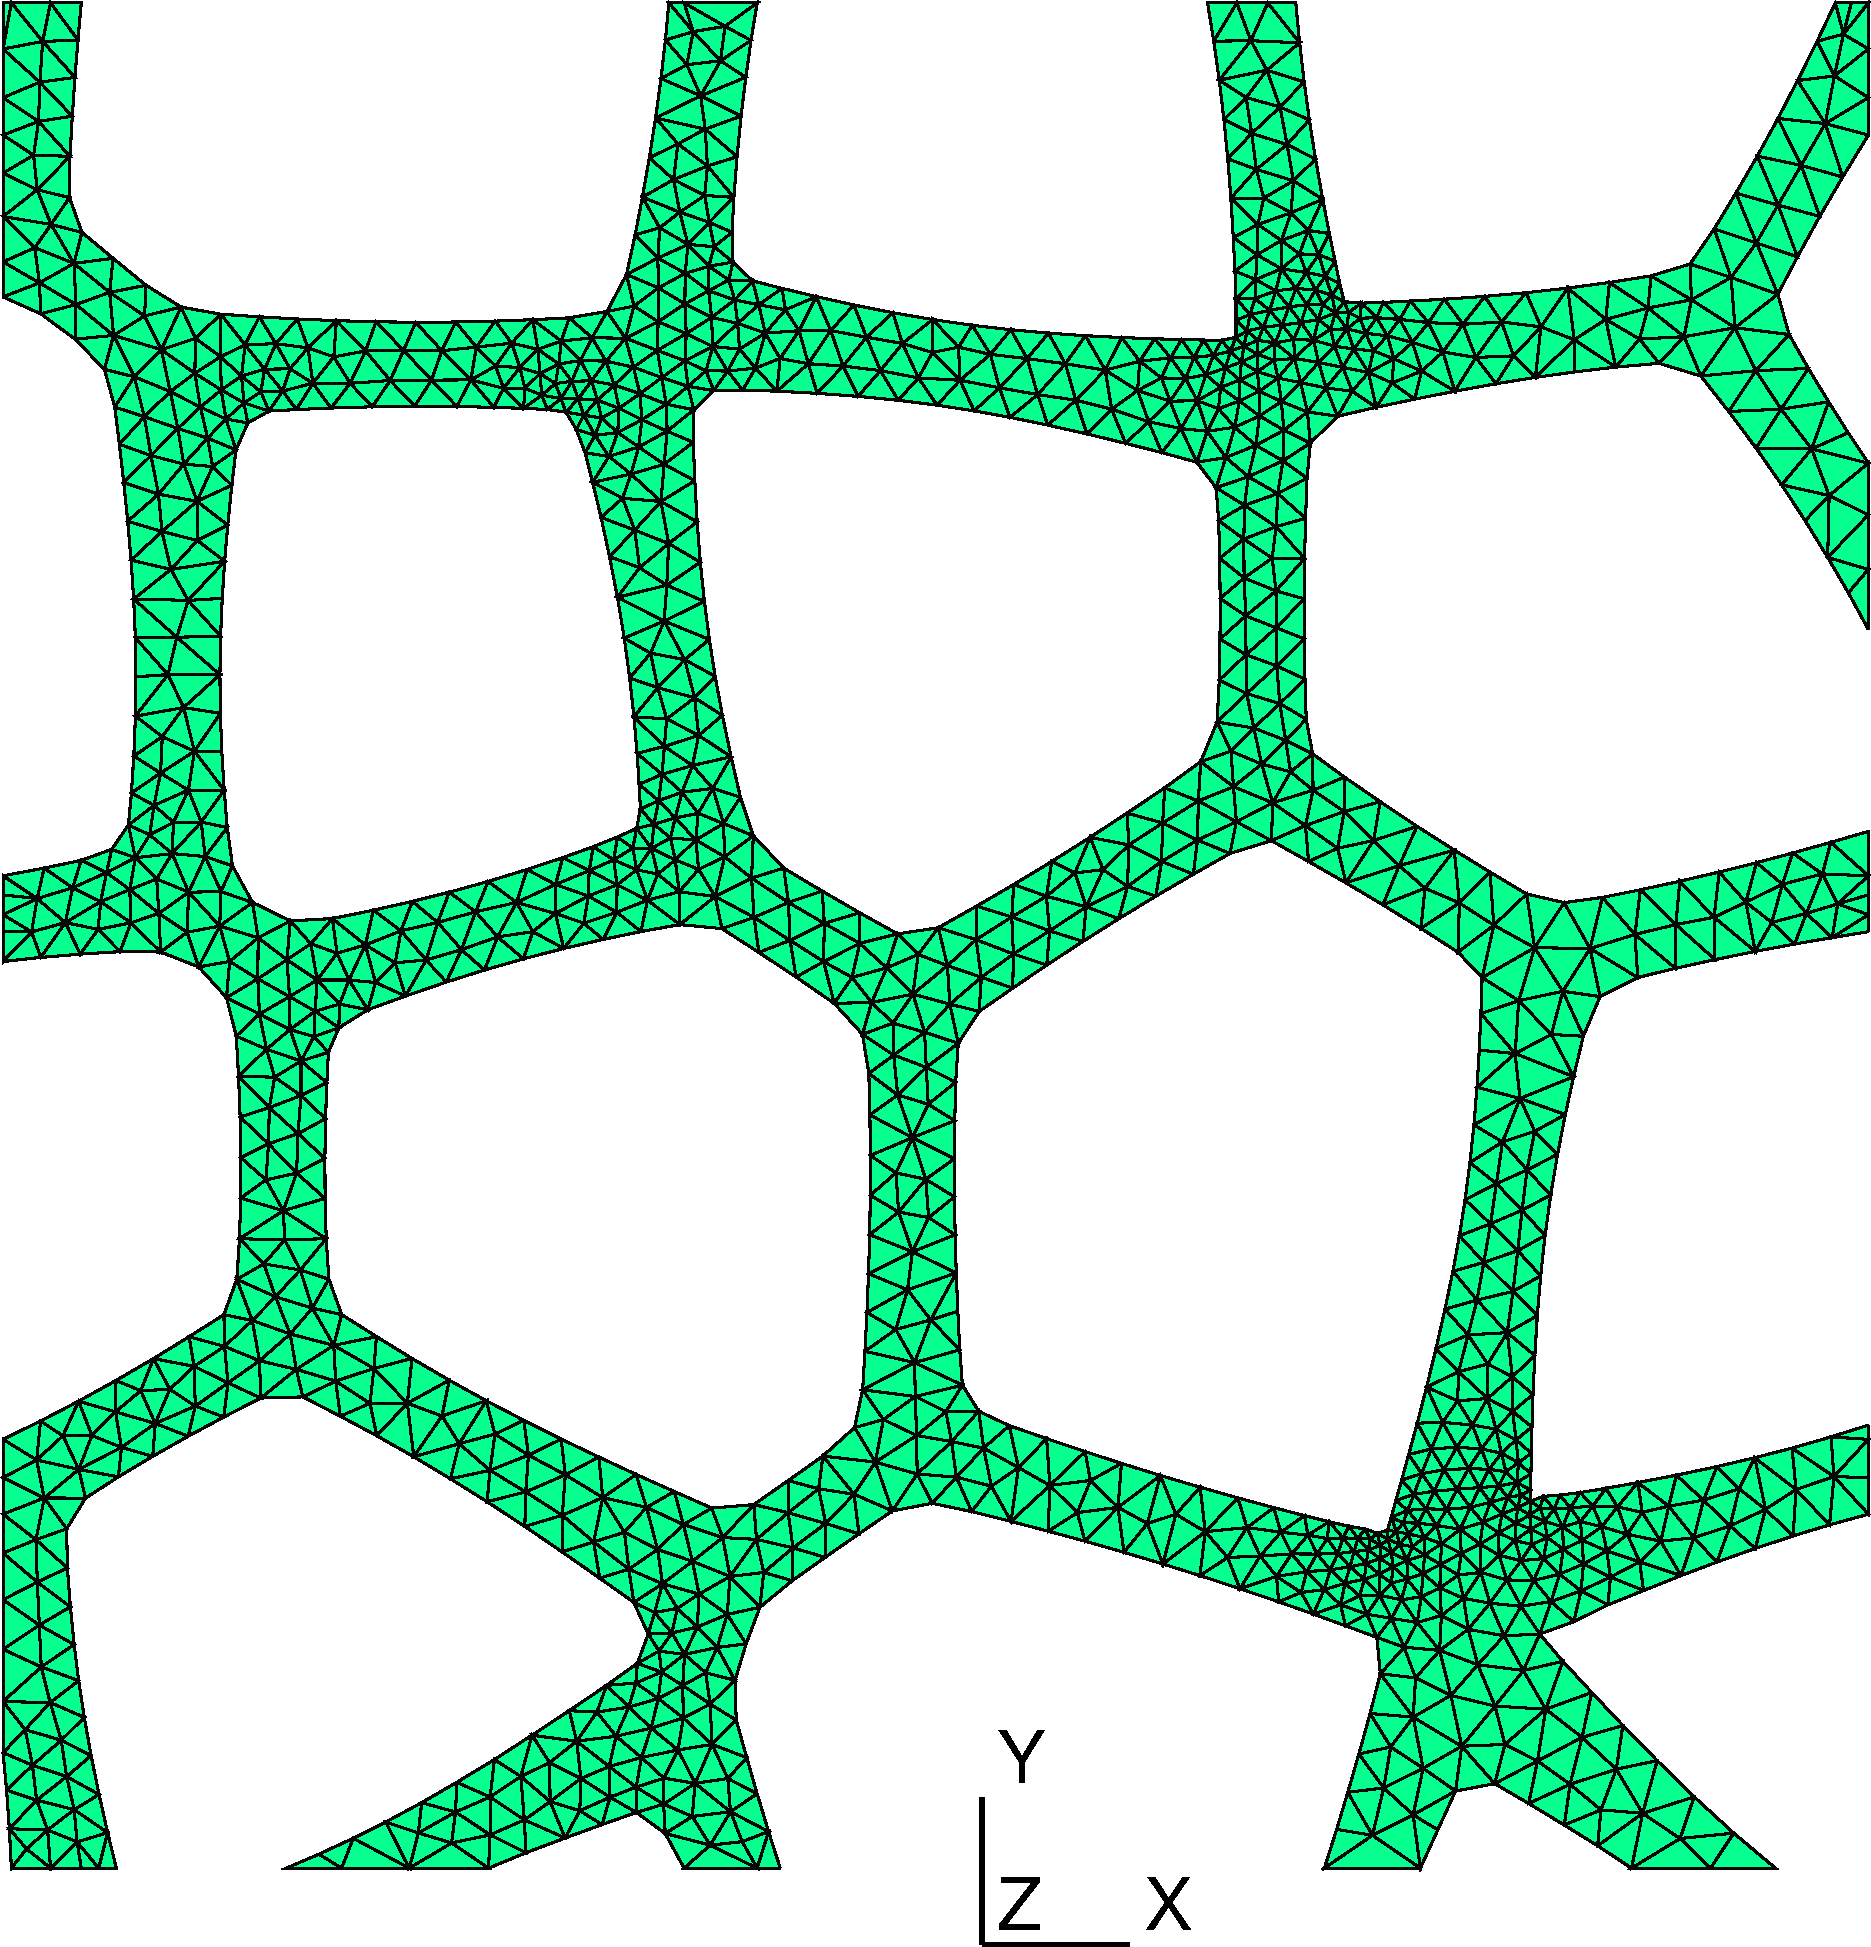
\includegraphics[width=6cm]{rve_clusterno_3}
		\caption{}
	\end{subfigure}
	\begin{subfigure}[t]{0.45\textwidth}
		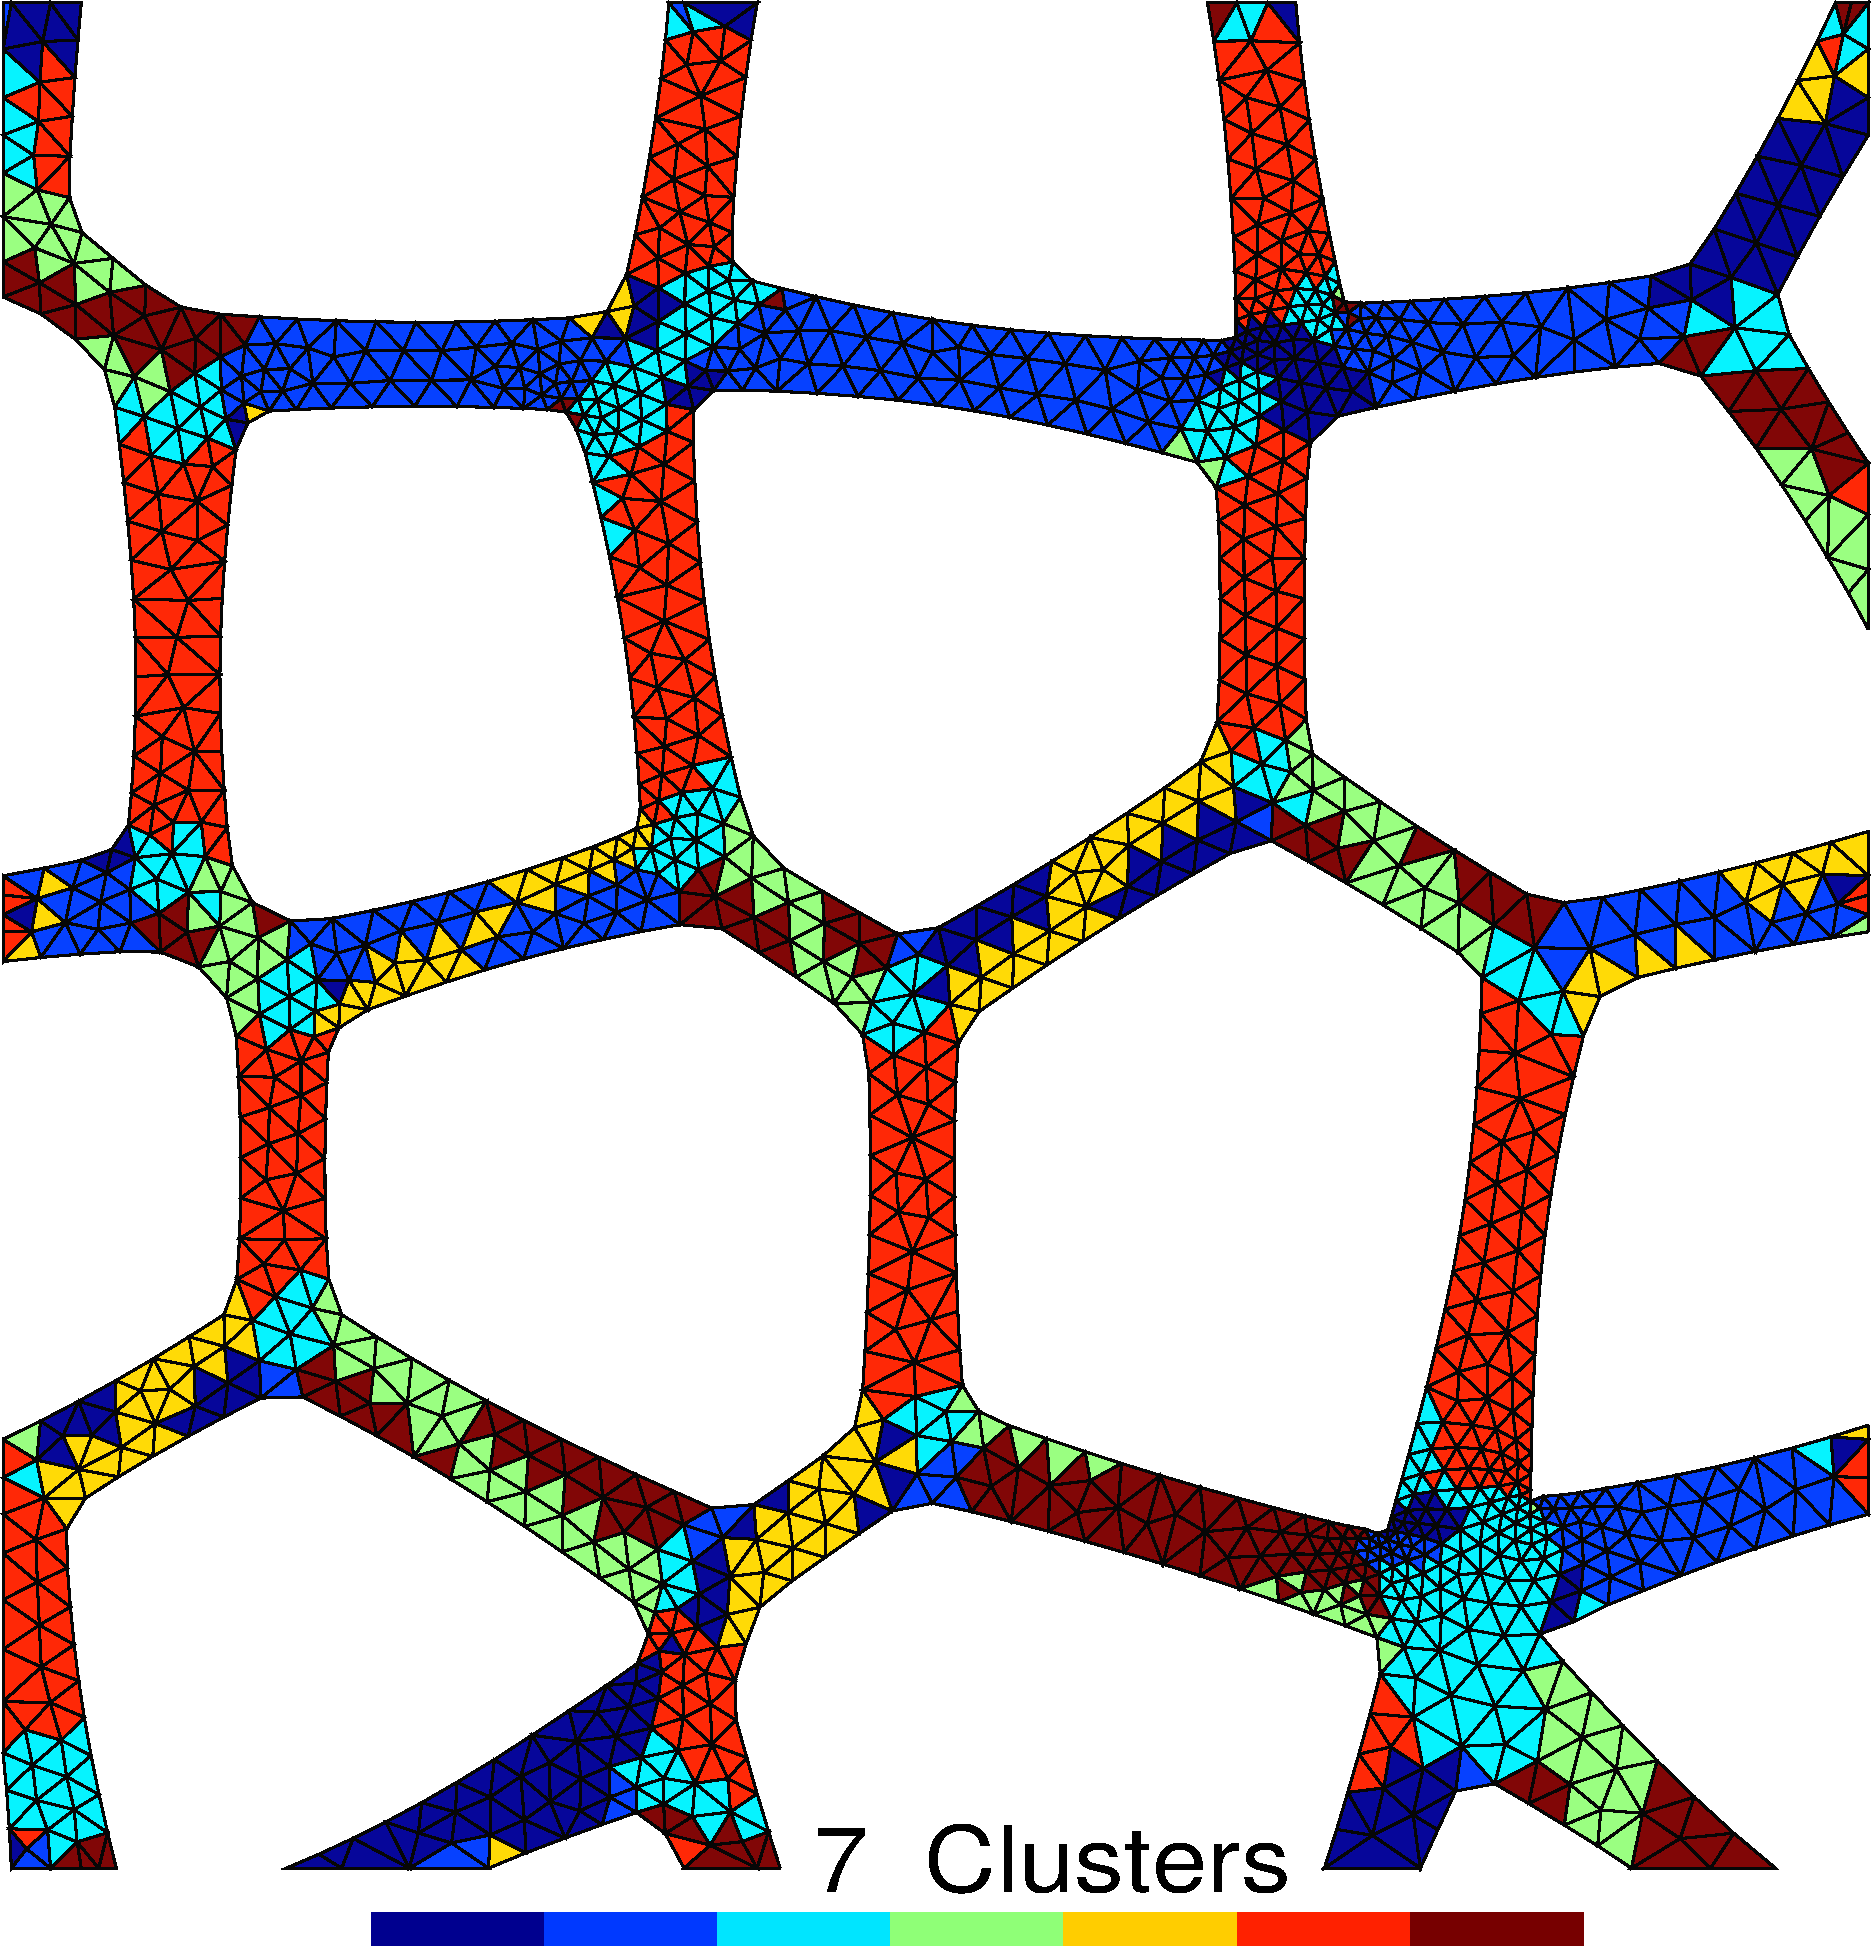
\includegraphics[width=6cm]{rve_cluster7_3}
		\caption{}
	\end{subfigure}
	\begin{subfigure}[t]{0.45\textwidth}
		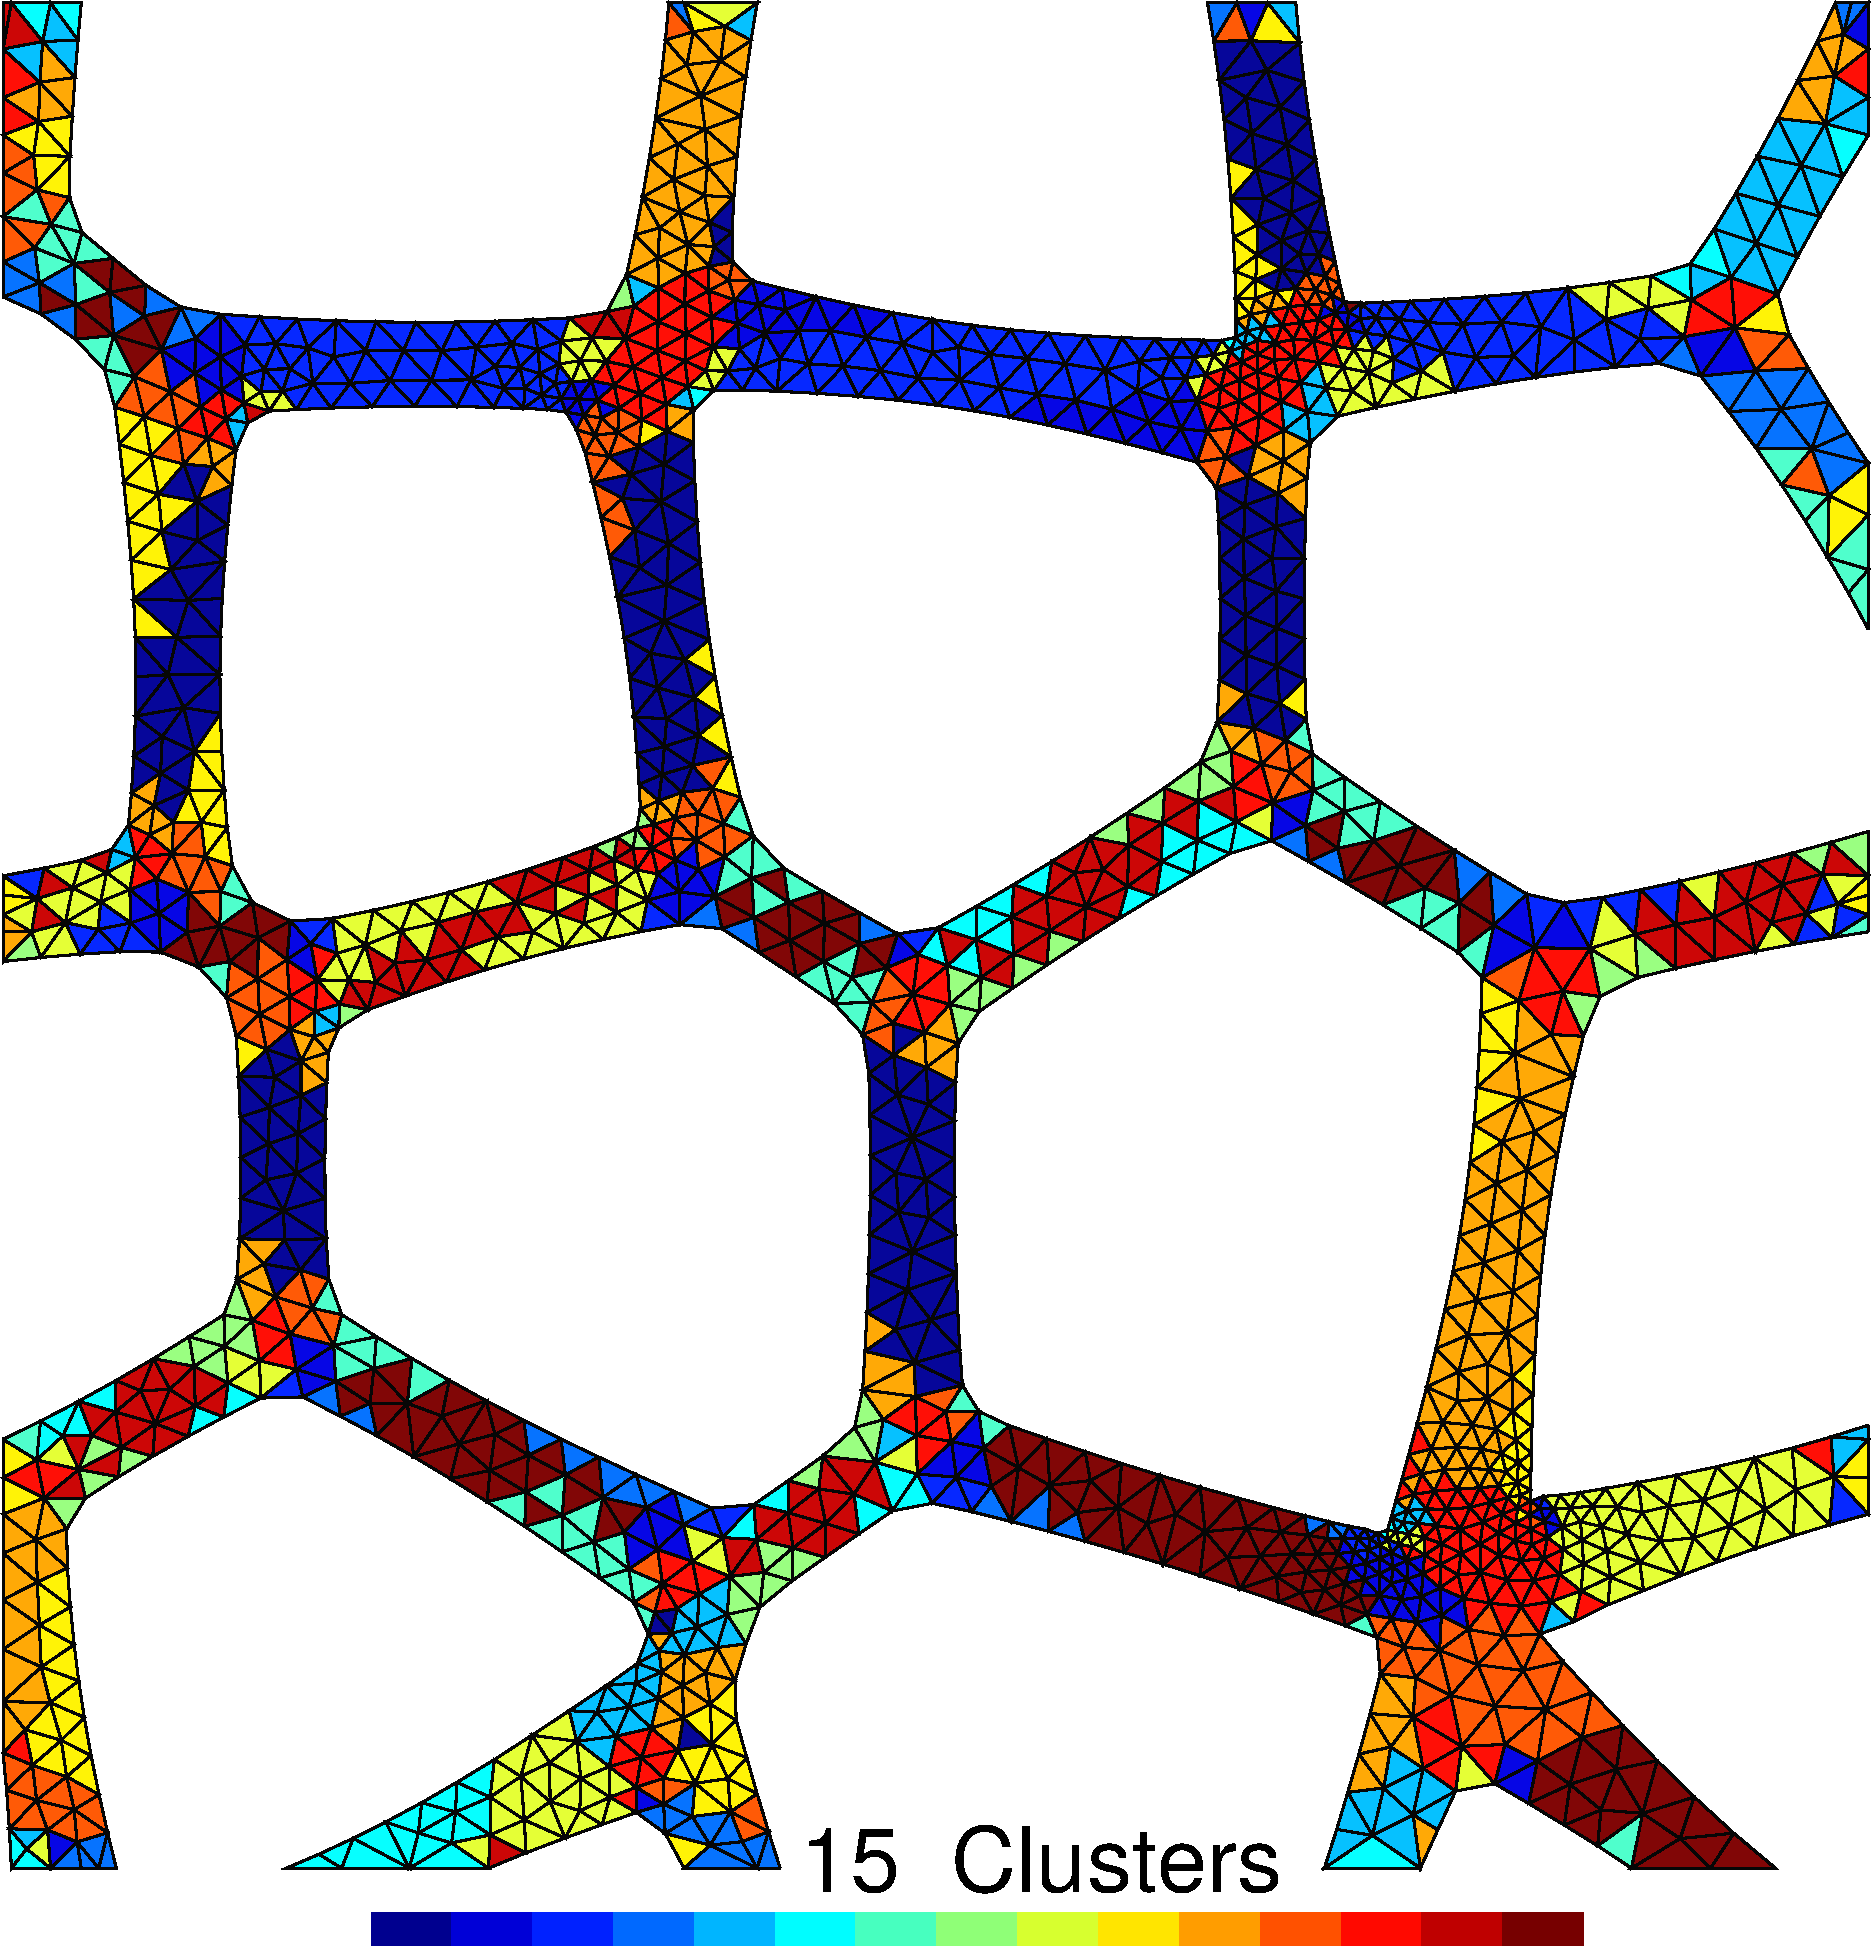
\includegraphics[width=6cm]{rve_cluster15_3}
		\caption{}
	\end{subfigure}
	\begin{subfigure}[t]{0.45\textwidth}
		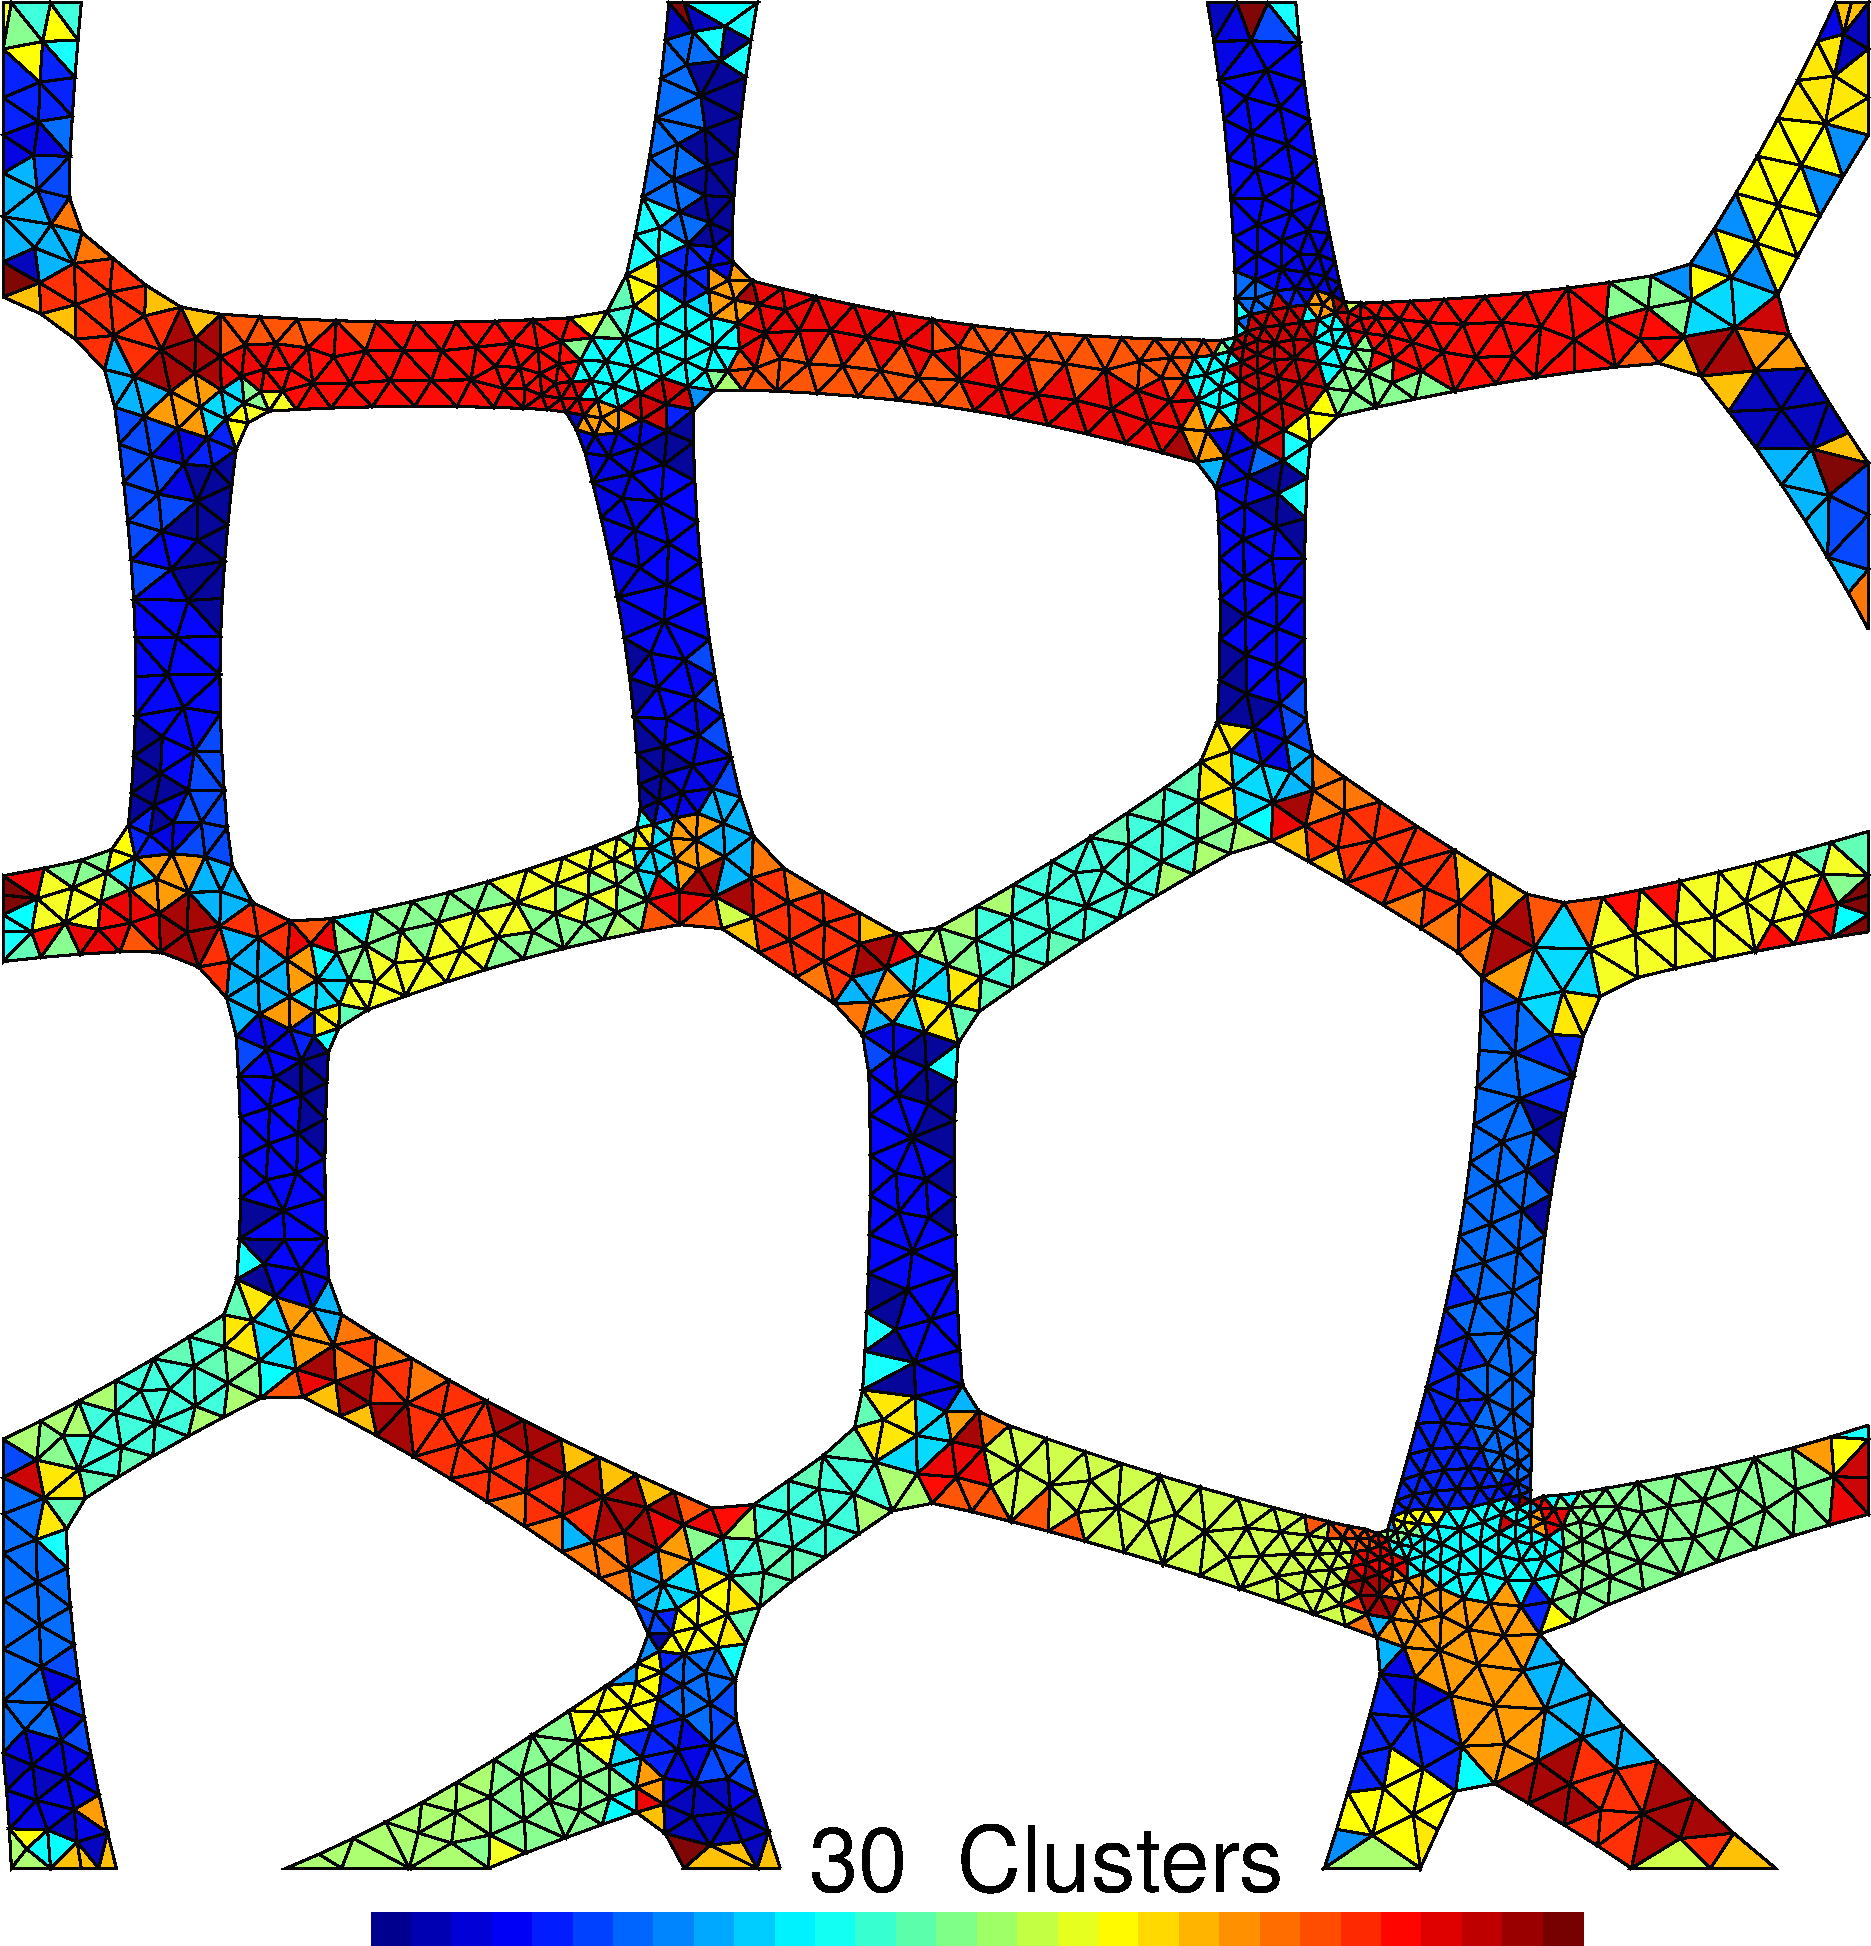
\includegraphics[width=6cm]{rve_cluster30_3}
		\caption{}
	\end{subfigure}
	\caption{Two dimensional $ k $-means clustering results of a 2D representation of an inclusion packing, (a) representing the discretized RVE, divided into (b) 7, (c) 15, and (d) 30 sub-domains, each individual domain in the RVE shown by the same color. }\label{fig-ch-cluster}
\end{figure}

By dividing the RVE into clustered sub-domains, the objective is to reduce the number of microscopic internal states that is necessary to efficiently represent the history dependence of the microscopic BVP given by Eq. (\ref{eq-ch-state5}) all while ensuring maximum information retention. $ k $-means clustering basically involves:
\begin{itemize}
	\item Evaluation of the strain concentration at each point in the domain: 
	A strain concentration tensor $ \mathbb{A}(\textbf{x}) $ at each point in the micro domain is related by
	\begin{equation}\label{eq-ch-cluster1}
		\tgmm[]{F}(\textbf{x})=\mathbb{A}(\textbf{x}):\tgm[]{F};
	\end{equation}
	\item Group the points into $ k $ clusters with minimal difference in strain concentration at each point compared to the average value inside the cluster: A cluster $ j\in k $ contains all the points in the domain whose strain concentration tensor $ \mathbb{A}(\textbf{x}) $ is the closest to the average  $ \mathbb{A}_j $ of the cluster than to that of any other cluster $ i $,  $ \mathbb{A}_i$, with $ i\ne j $. Thus the objective of $ k $-means clustering is to calculate the least square sums $ \mathcal{S} $ within the cluster for the $ k $ sets, $ \mathcal{S}=\{S_1,S_2,...,S_k\} $ by using the Frobenius norm to obtain the shape of the clusters:
	\begin{equation}\label{eq-ch-cluster2}
	\mathcal{S}=\underset{\mathcal{S}'}{\arg\min}\sum_{j=1}^{k}\sum_{n\in S_j}^{}\left|\left|\mathbb{A}_n-\mathbb{A}_j\right|\right|^2
	\end{equation}
	with strain concentration tensor $ \mathbb{A}_n $ at the $ n $th data point and the mean of all the strain concentration tensors $ \mathbb{A}_j $ at the mean points within a cluster $ S_j $;
	\item Once the clusters are identified, an average internal state $ {\tgmm[]{Z}}_j $ for each cluster can be computed as
	\begin{equation}\label{eq-ch-cluster3}
	{\tgmm[]{Z}}_j=\frac{1}{\omega_j}\int_{\omega_j}\tgmm[]{Z}d\omega.
	\end{equation}
	This average internal state can then be substituted in Eq. (\ref{eq-ch-state5}) to obtain the reduced form
	\begin{equation}\label{eq-ch-cluster4}
	\tgm[]{Z}=[{\tgmm[]{Z}}_j\ \ \text{for}\ j=1...k].
	\end{equation}
\end{itemize}
The degree of data compression achieved is dependent on the choice of the number of clusters $ k $. A higher number of clusters increases the amount of information that needs to be stored to be used in the online stage that also increases the cost of computation along with the accuracy of predictions, thereby necessitating a selection that balances the two. A point to note is that the average internal state based on volume averaging is not a replacement for the homogenized internal variable due to the necessity to supplement the volume averages with physical arguments to ensure the overall energy consistency\cite{berrymanComparisonUpscalingMethods2005}.

\section{Monotonic proportional loading conditions}\label{nn-mono}

As a first case of study, the adaptability of the FNN models on a monotonic loading case, or a uni-directional loading case is studied. The underlying assumption behind this study is that a unidirectional monotonic and proportional loading, that does neither change nor reverse the deformation direction, ensures that there is no history dependent behavior, thus keeping the case study simple enough. A similar approach has been studied in \cite{fritzenOntheflyAdaptivityNonlinear2019} where an FNN was trained to be used as a surrogate that is a highly efficient constitutive relation for a nonlinear material similar to the one that is being studied. Based on similar strategy, an efficient FNN is trained to predict the behavior of the material in terms of its stress response, if possible, at every integration point for a given effective strain.

In this Section, the generated training datasets from Section \ref{nn-gendata} will be suitably prepared to be used with the FNN models. The link between the surrogate FNN and the corresponding constituent law in an \fee method will be demonstrated. The strategy to train the FNN models will be presented before discussing some of the aspects of the results.

%\subsection{Input and Output parameters of the ANN}\label{nn-mono-io}
%Considering that the micro-scale BVP presented in Chapter \ref{chap-ch} respects frame indifference, the Green-Lagrangian strain tensor $ \tgm[]{E} $ and the 2$ ^\text{nd} $ Piola-Kirchhoff stress tensor $ \tgm[]{S} $ negates the necessity of the rigid rotation mode. By describing the stress-strain relationship by $ \tgm[]{E} $ and $ \tgm[]{S} $, the plane strain condition system can be reduced to the input $ \textbf{\textit{u}}=\{E_{\text{M}_{XX}},E_{\text{M}_{YY}},E_{\text{M}_{XY}}\} $ with the output as $ \textbf{\textit{u}}=\{S_{\text{M}_{XX}},S_{\text{M}_{YY}},S_{\text{M}_{ZZ}},S_{\text{M}_{XY}}\} $. Consequently it becomes important to obtain the required input values $ \tgm[]{E} $ from $ \tgm[]{F} $ to train the ANN and also to obtain $ \tgm[]{P} $ from $ \tgm[]{S} $ to be subsequently fed to the macro-scale analysis, simply by
%\begin{eqnarray}\label{eq-nn-io}
% \tgm[]{E} & = \frac{1}{2}\left(\tgm[]{F}^T\cdot\tgm[]{F}-\textbf{I}\right)\\
% \tgm[]{P} & = \tgm[]{F}\cdot\tgm[]{S}.
%\end{eqnarray}
%To facilitate the macro-scale simulation, the necessary material parameter tensor in ht macro-scale, $ \mathbb{C}_\text{M} $ can be simply obtained as $ \partial\tgm[]{S}/\partial\tgm[]{E} $ using the implicit based differentiation unctions available in the API repositories used to train the models.

%\subsection{Generation of data}\label{nn-mono-data}

\subsection{Preparation of Datasets for FNN}\label{nn-mono-datapre}
Generally, FEM simulations accept the strain-state sequence
\begin{equation}\label{eq-nn-data1}
\tgm[]{U}^i = \left[{\tgm[]{U}^i}_0,{\tgm[]{U}^i}_1,...,{\tgm[]{U}^i}_{N_{s}}\right],
\end{equation}
to generate stress states in a sequential format as%and
\begin{equation}\label{eq-nn-data2}
\tgm[]{P}^i = \left[{\tgm[]{P}^i}_0,{\tgm[]{P}^i}_1,...,{\tgm[]{P}^i}_{N_{s}}\right]
\end{equation}
where 
%$ {\tgm[]{E}^i}_0 $ and 
$ {\tgm[]{U}^i}_0 $ and 
$ {\tgm[]{P}^i}_0 $ is 
the right stretch tensor and the 1$ ^\text{st} $ Piola-Kirchhoff stress tensor respectively, $  {\tgm[]{U}^i}_0=\textbf{I} $ is the starting value of the evaluation path, and $ N_s $ denotes the number of steps. Both the FEM inputs and the outputs can be saved in the sequential format in which it is generated. However, an FNN can be trained simply with individual stress-strain states and for this reason, all the stress-strain states resulting from all the training simulations can be arranged in a single variable. So, once the training data is collected, one can obtain the right stretch strain tensor $ \tgm[]{E} $ and the 2$ ^\text{nd} $-Piola Kirchhoff stress tensor $ \tgm[]{S} $ from Eqs. (\ref{eq-nn-io}) - (\ref{eq-nn-io-1}) and stack them together in the following manner:
\begin{eqnarray}\label{eq-nn-data3}
\tgm[]{E}^{FNN}=\left[..,\tgm[]{E}^{i-1},\tgm[]{E}^i,\tgm[]{E}^{i+1},..\right] = 
\left[..,{\tgm[]{E}^{i-1}}_0,{\tgm[]{E}^{i-1}}_1,...,{\tgm[]{E}^{i-1}}_{N_{s_{i-1}}},\right.\nonumber\\
{\tgm[]{E}^i}_0,{\tgm[]{E}^i}_1,...,{\tgm[]{E}^i}_{N_{s_i}},
\left.{\tgm[]{E}^{i+1}}_0,{\tgm[]{E}^{i+1}}_1,...,{\tgm[]{E}^{i+1}}_{N_{s_{i+1}}},..\right],
\end{eqnarray}
\begin{eqnarray}\label{eq-nn-data4}
\tgm[]{S}^{FNN}=\left[..,\tgm[]{S}^{i-1},\tgm[]{S}^i,\tgm[]{S}^{i+1},..\right] = 
\left[..,{\tgm[]{S}^{i-1}}_0,{\tgm[]{S}^{i-1}}_1,...,{\tgm[]{S}^{i-1}}_{N_{s_{i-1}}},\right.\nonumber\\
{\tgm[]{S}^i}_0,{\tgm[]{S}^i}_1,...,{\tgm[]{S}^i}_{N_{s_i}},
\left.{\tgm[]{S}^{i+1}}_0,{\tgm[]{S}^{i+1}}_1,...,{\tgm[]{S}^{i+1}}_{N_{s_{i+1}}},..\right],
\end{eqnarray}
where $ i= 1,...,N_{samples} $ with $ N_{samples} $ denoting the total number of sample sequences, and $ N_{S_i} $ denotes the number of steps in each training sample sequence, $ i $. In a sequential training with FNN where the assumption that a monotonic loading will result in a single stress state for any given strain state combination, the data from multiple simulations can be stacked over each other and fed in batches to the ANN. 


\subsection{Material Law with FNN}\label{nn-mono-material}
The idea behind using the FNN as a surrogate for the micro-scale BVP is to replace the constitutive relations that arise from the resolution of the microscopic BVP on an RVE by an FE resolution. The traditional FEM solver converges at every strain state before proceeding towards the next time step and generates the homogenized stress states. 
From Eqs. (\ref{eq-dG-const_macro}), (\ref{eq-nn-io}) and (\ref{eq-nn-io-1}), for a monotonic loading case the mechanical behavior at any time step $ n $ can be explicitly modeled by the constitutive law as
\begin{equation}\label{eq-nn-law1}
{\tgm[]{S}}_n=\mathcal{S}({\tgm[]{E}}_n)\quad n=1,...,N_{s_i}\text{ and }i=1,..,N_{samples}
\end{equation}
For FNNs, Eq. (\ref{eq-nn-law1}) can be written as
\begin{equation}\label{eq-nn-law2}
\tgm[]{S}^{FNN}=\mathcal{S}^{FNN}(\tgm[]{E}^{FNN};\textbf{W}^S_{FNN})
\end{equation}
where $ \mathcal{S}^{FNN} $ the corresponding ANN based surrogate, $ \textbf{W}^S_{FNN} $ are the parameters of the network. Eq. (\ref{eq-nn-law2}) is analogous to Eq. (\ref{eq-nn-func}) that presents a global ANN system with the input $ \textbf{\textit{u}}=\tgm[]{E}^{FNN} $ and the output $ \textbf{\textit{v}}=\tgm[]{S}^{FNN} $.

The training of the FNN involves the initialization of the parameters of the network, $ \textbf{W}^P_{FNN} $ and subsequent optimization using the training datasets, $ \left[\tgm{E}^{FNN},\tgm{S}^{FNN}\right] $, to reduce the mean square error as explained in Section \ref{nn-ann-train}.

\subsection{Online computation with trained FNN}\label{nn-mono-train}
Once the FNNs have been trained, they can be used online as a surrogate for the micro-scale BVP of the \fee method. However, considering that the FNNs have been trained with datasets that are not directly used in the FEM computation, these values have to be reversed suitably so that the predicted values of the FNN models represent the desired values.

This process is quite simple for FNNs that have been used to study the behavior of material models under proportional loading. At any stage $ t $ of the computation, for a given deformation $ {\tgm{F}}_t $ one can obtain,
\begin{equation}\label{eq-fnn-1}
{\tgm{U}}_t=\sqrt{{\tgm{F}}_t^T\cdot{\tgm{F}}_t},
\end{equation}
and 
\begin{equation}\label{eq-fnn-2}
{\tgm{E}}_t=\frac{1}{2}\left({\tgm{U}}_t^2-\textbf{I}\right).
\end{equation}
With the trained parameters $ \textbf{W}^P_{FNN} $, one can obtain the predicted value,
\begin{equation}\label{eq-fnn-3}
{\tgm{S}}_t^P=\mathcal{S}^{FNN}({\tgm{E}}_t;\textbf{W}^S_{FNN}),
\end{equation}
and
\begin{equation}\label{eq-fnn-4}
{\tgm{P}}_t^P={\tgm{F}}_t\cdot{\tgm{S}}_t^P.
\end{equation}
A point to note here is that the ANN models are generally trained with normalized values and for this reason one has to ensure that the features to be predicted are scaled before and after feeding into the FNN model.

\subsection{Prediction of FNN surrogates}\label{nn-mono-results}
To study the behavior of the FNN model trained for proportional loading datasets, a set of simulations have been performed. A 2D FE model of a representative foam as explained in Section \ref{app-geom} was used to simplify the computational load on the study. 

\subsubsection{Preparation of Datasets}
The datasets consisting of stress-strain states are generated by selecting $ \lambda_1 $ and $ \lambda_2 $ as described in Section \ref{nn-gendata-prop} with the upper bound $ R_\text{max}=0.4 $. The material properties described in Section \ref{res-fem} are applied here as well. The minimum incremental strain $ \Delta{\tgm{U}}_\text{min}=0.0025 $ is chosen to ensure as much of the strain space is covered by the simulations. The generated data is such that the maximum and minimum bounds of the right stretch tensor are
\begin{eqnarray}\label{eq-fnn-res1}
\textbf{E}_\text{min}&=&\min\left(E_{XX}^{FNN},E_{XY}^{FNN},E_{YY}^{FNN}\right)\nonumber\\&=&\left[-0.28037704, -0.14510625, -0.31417825\right]\nonumber
\end{eqnarray}
and
\begin{eqnarray}\label{eq-fnn-res2}
\textbf{E}_\text{max}&=&\max\left(E_{XX}^{FNN},E_{XY}^{FNN},E_{YY}^{FNN}\right)\nonumber\\&=&\left[0.4120193 , 0.14403125, 0.42864995\right].\nonumber
\end{eqnarray}


\begin{figure}
	\centering
	\begin{subfigure}[t]{0.75\textwidth}
		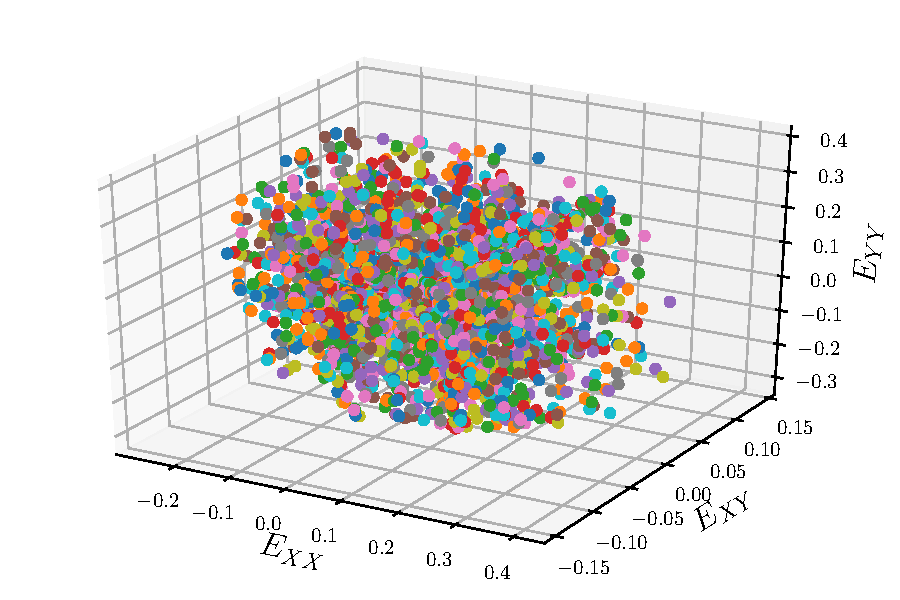
\includegraphics[width=\textwidth]{FNN_Random_States}
	\end{subfigure}
	\caption{A sample of strain-states used to train the FNN model. In general, the bigger the loading upper bound, more data is necessary to ensure the entire domain of strain-states is captured.}\label{fig-nn-fnn1}
\end{figure}

\begin{figure}
	\centering
	\begin{subfigure}[t]{0.4\textwidth}
		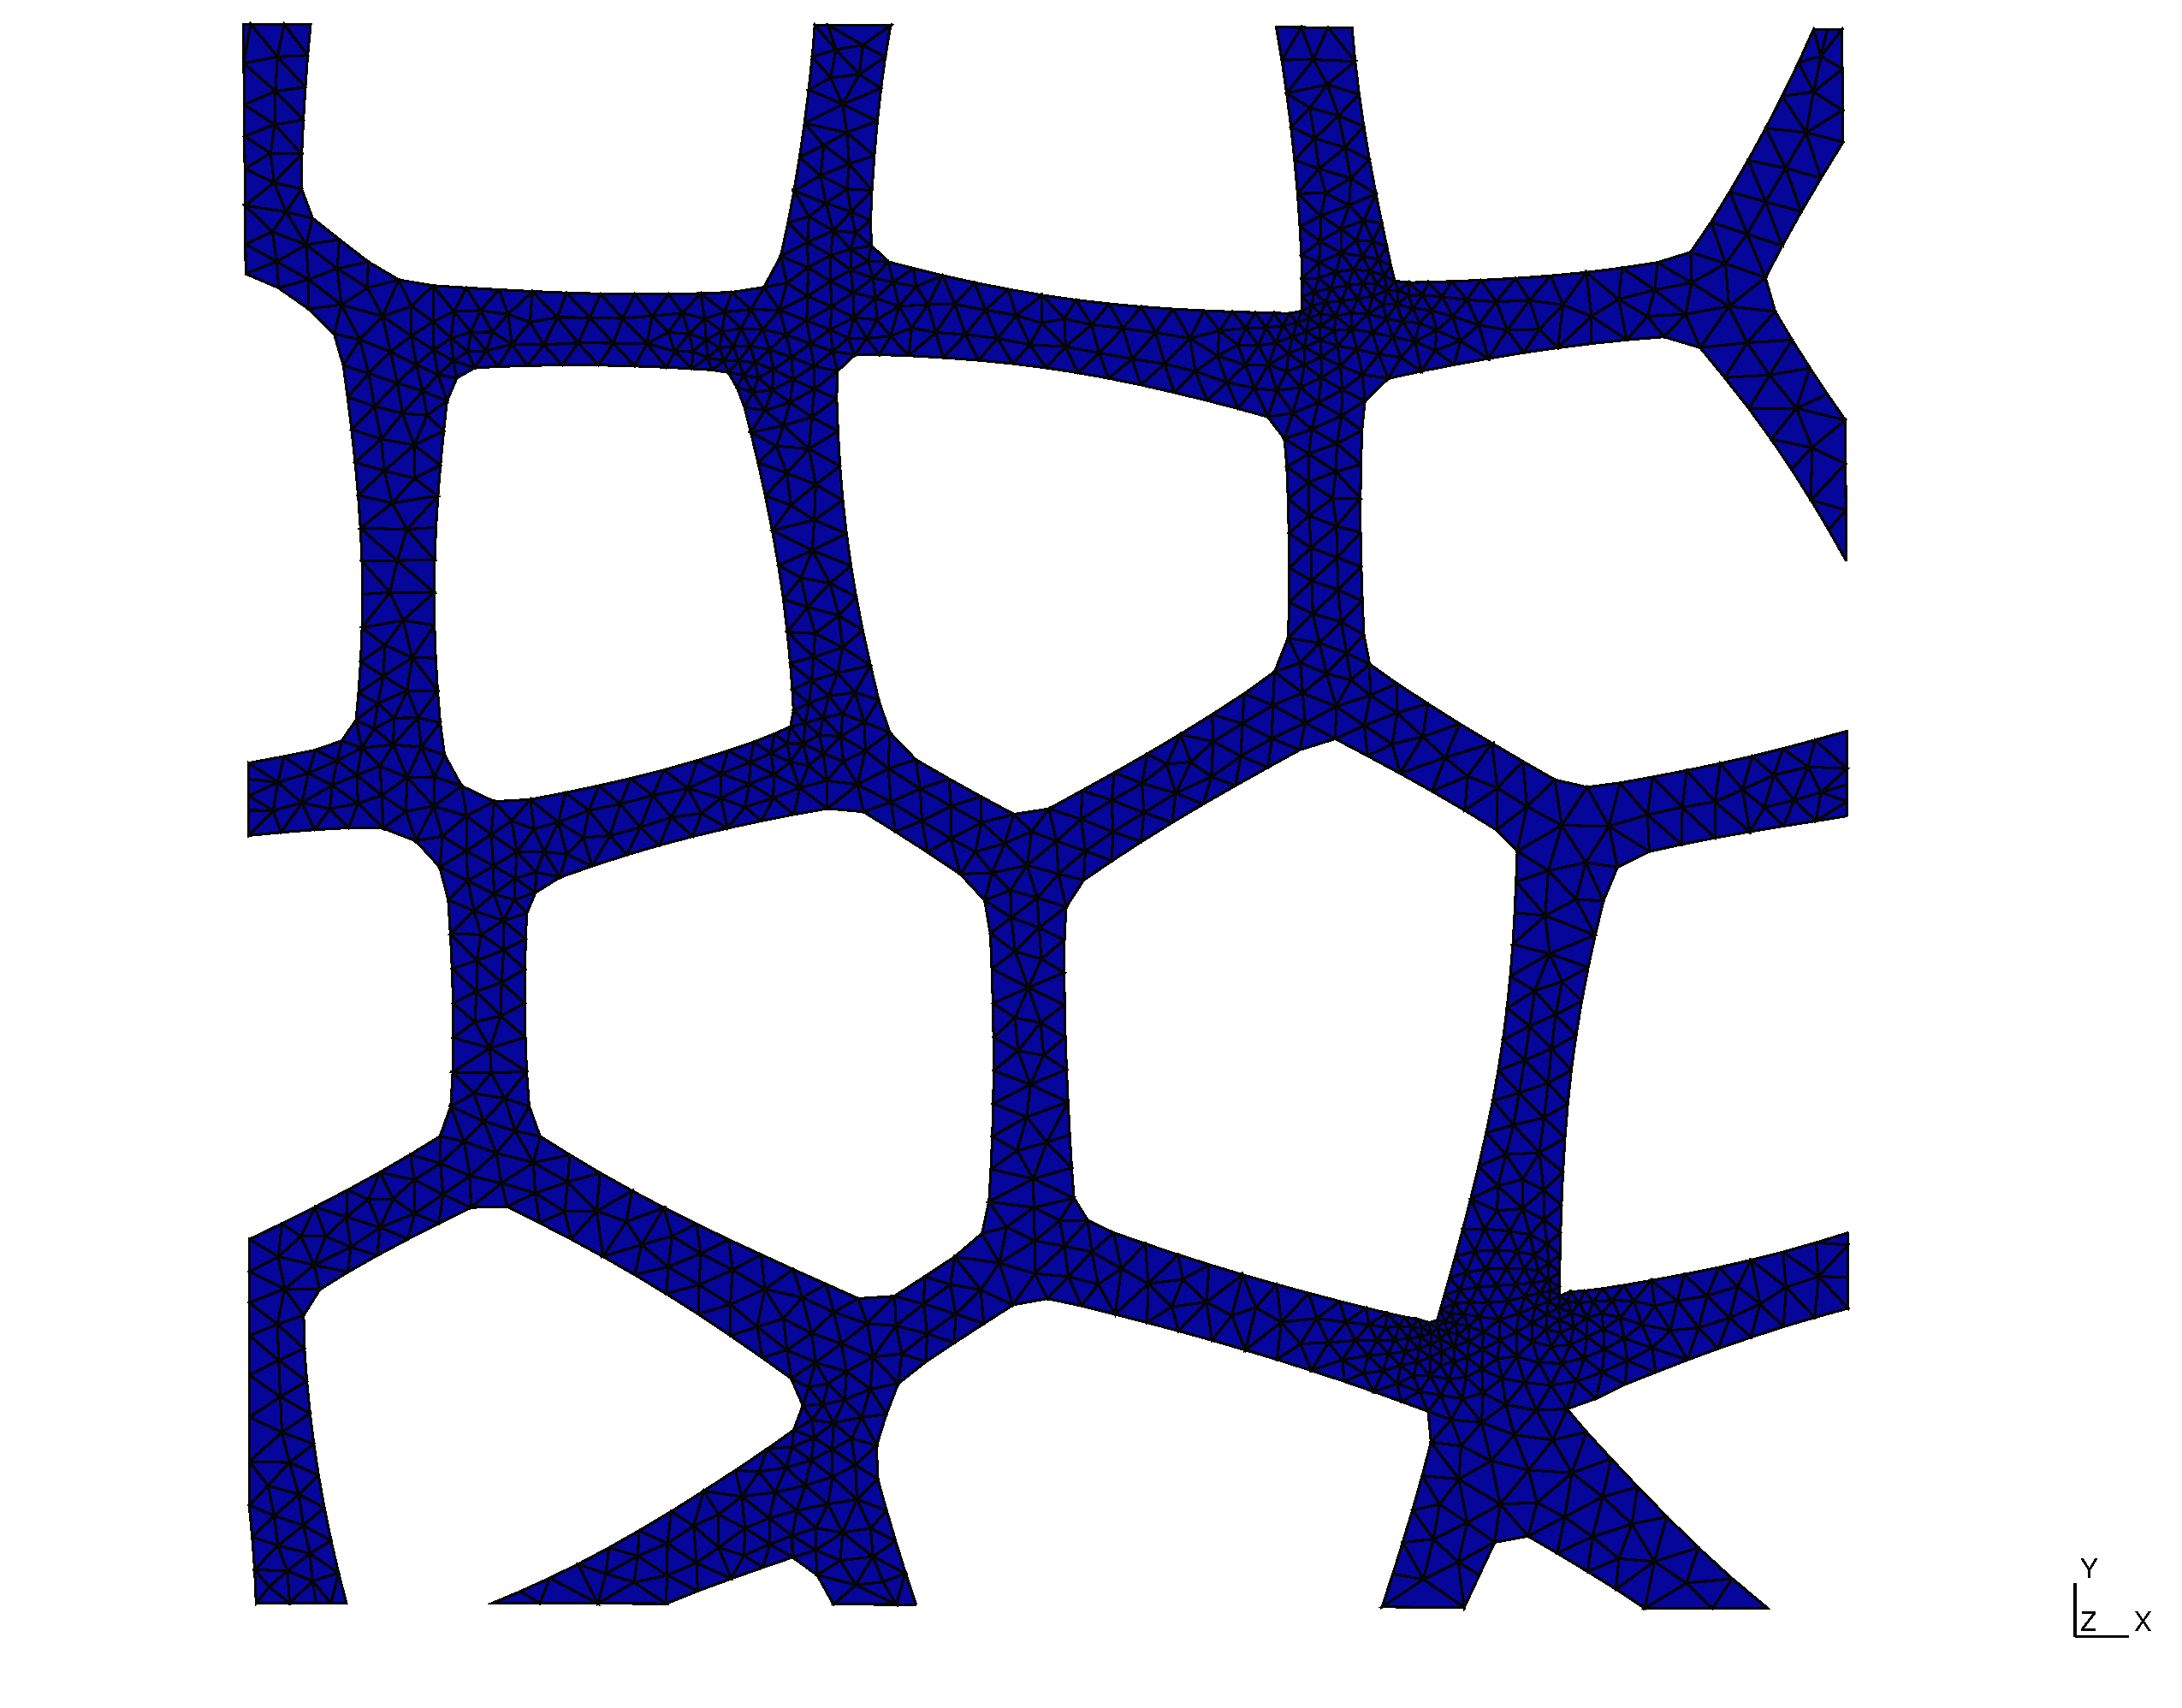
\includegraphics[height=5cm]{eqps_1}
	\end{subfigure}
	\begin{subfigure}[t]{0.4\textwidth}
		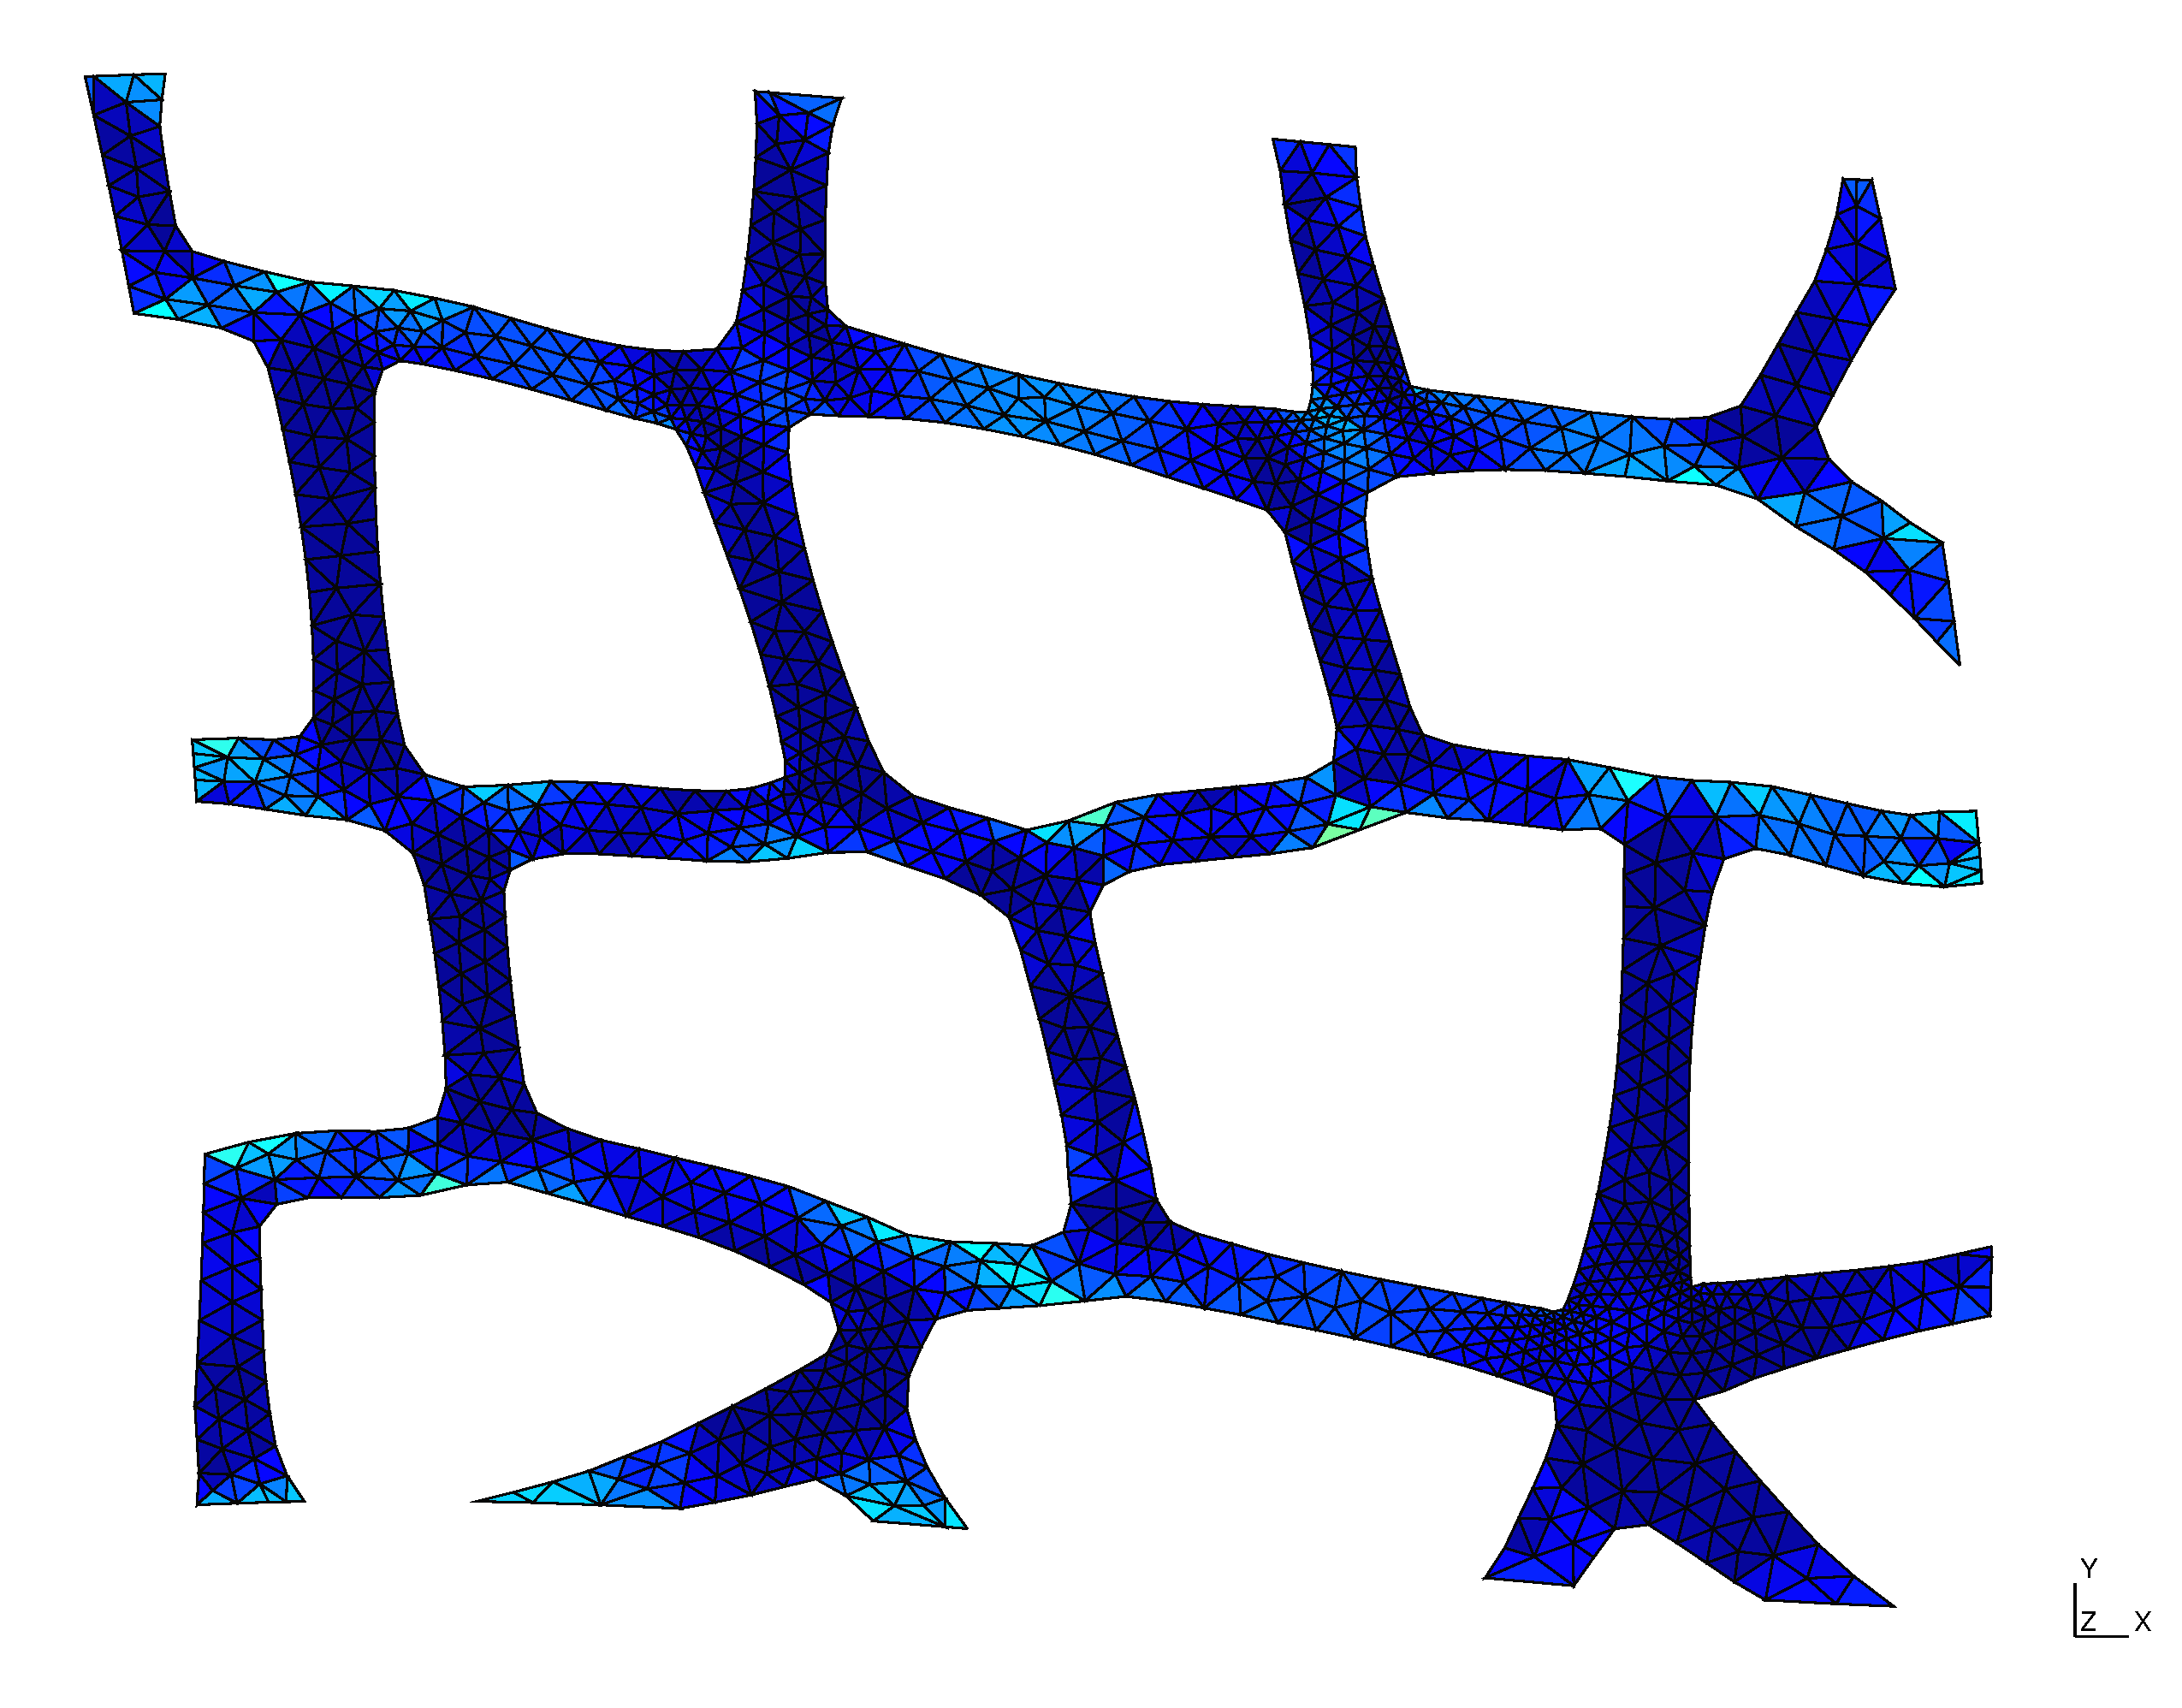
\includegraphics[height=5cm]{eqps_30}
	\end{subfigure}
	\begin{subfigure}[t]{0.4\textwidth}
		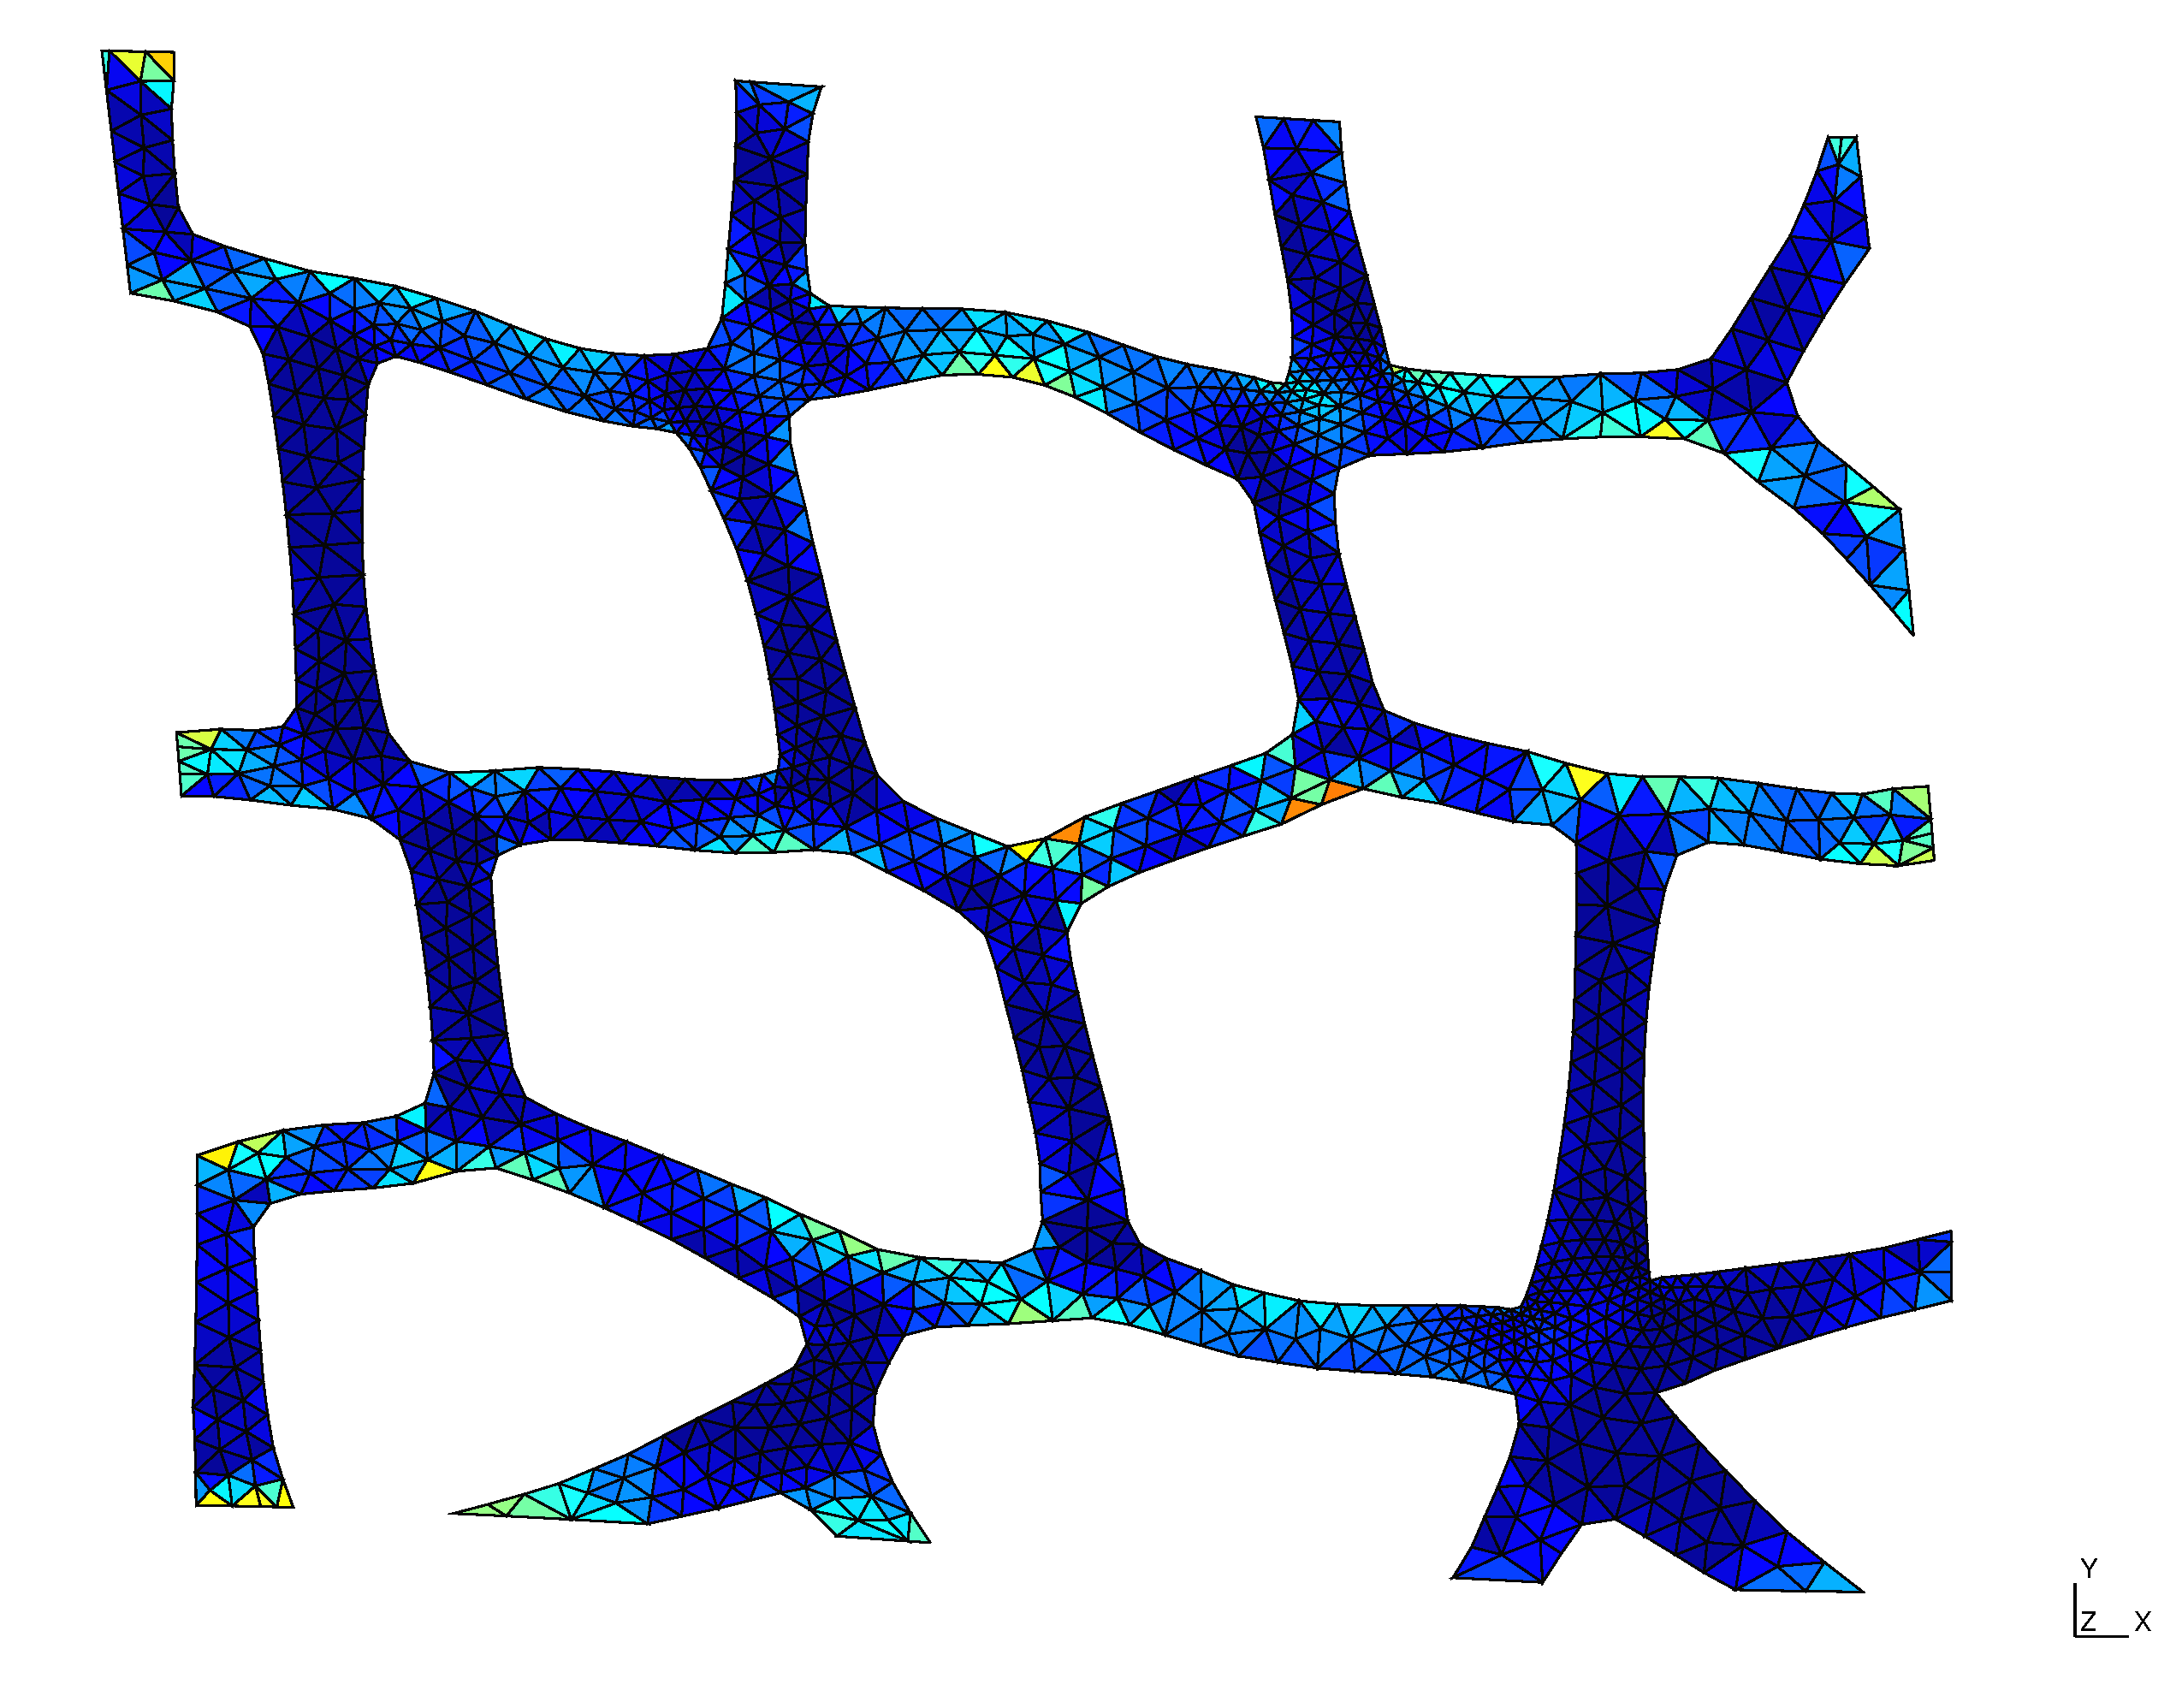
\includegraphics[height=5cm]{eqps_50}
	\end{subfigure}
	\begin{subfigure}[t]{0.4\textwidth}
		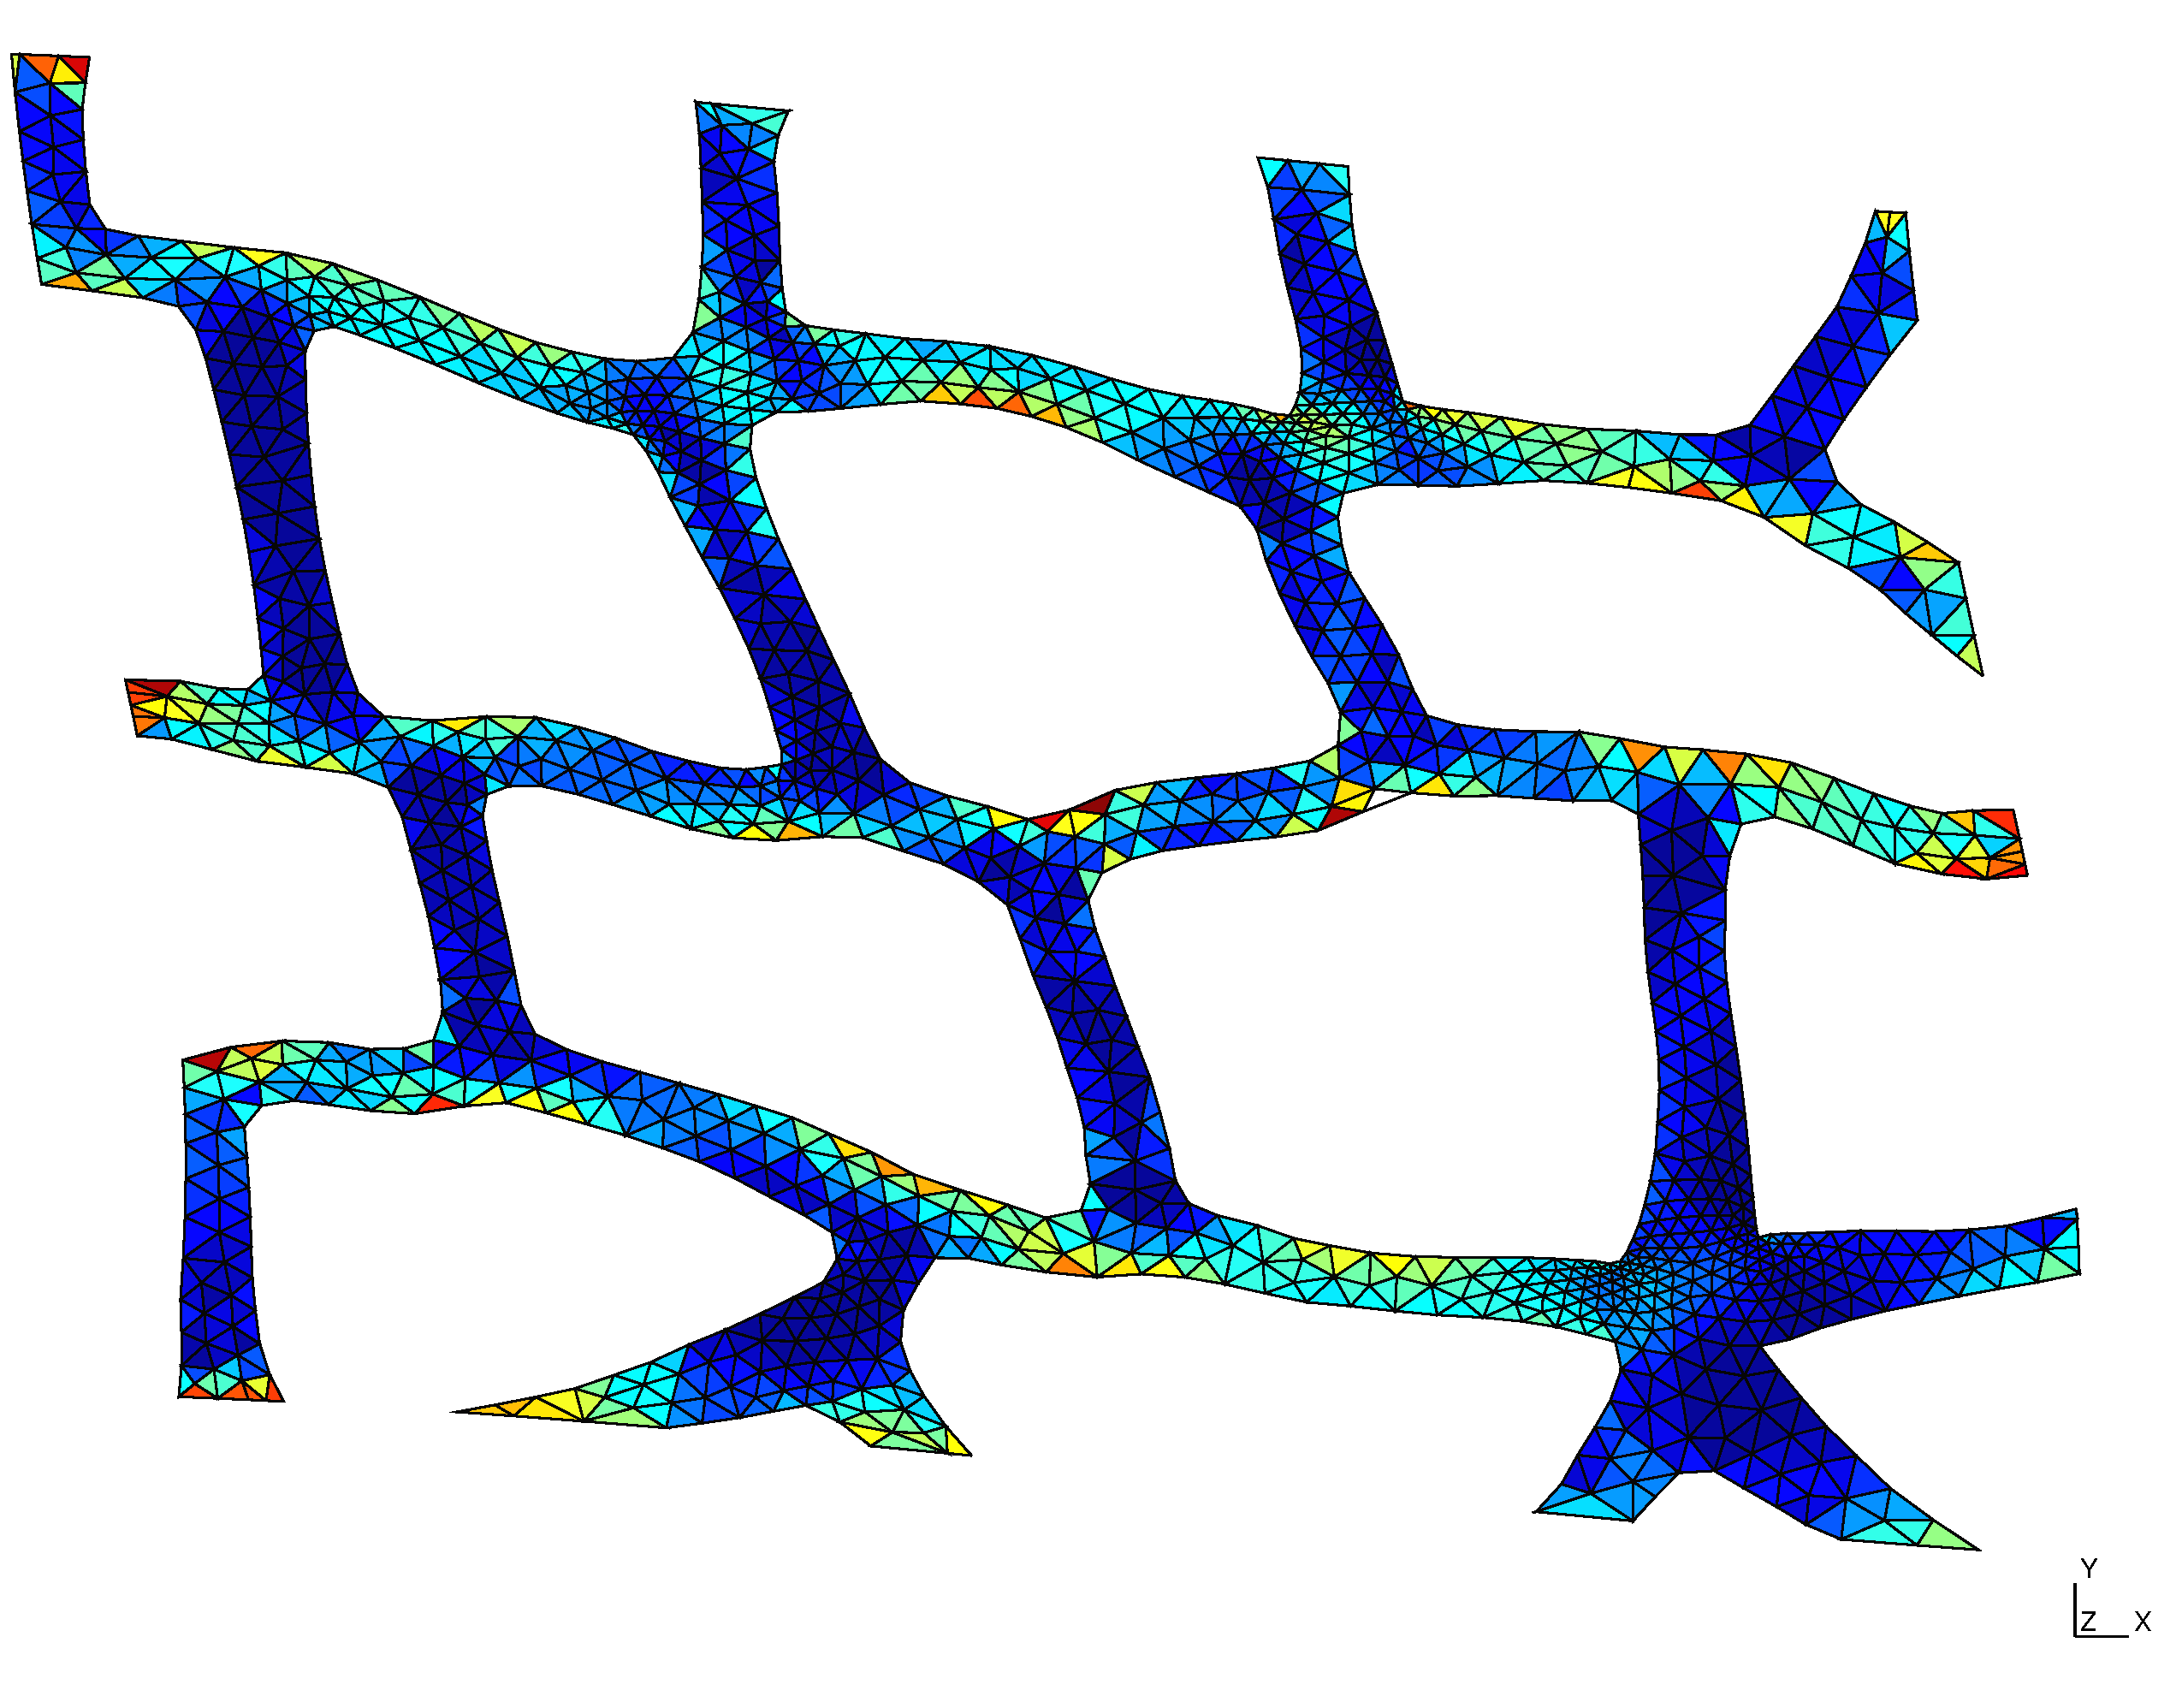
\includegraphics[height=5cm]{eqps_80}
	\end{subfigure}
	\begin{subfigure}[t]{0.45\textwidth}
	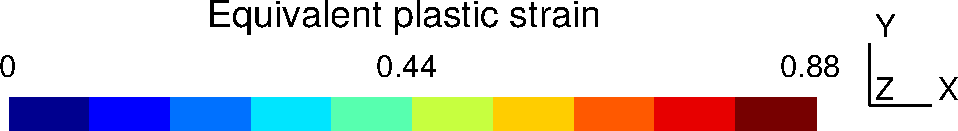
\includegraphics[width=\textwidth]{eqps_scale}
\end{subfigure}
	\caption{Snapshots of 4 stages of deformation as observed for a single sample numerical analysis under a monotonic proportional loading. The equivalent plastic strain is superimposed on the general deformation of the geometry.}\label{fig-nn-fnn1-1}
\end{figure}
Figure \ref{fig-nn-fnn1} illustrates some of the strain states generated as part of a large number of training sequences while Figure \ref{fig-nn-fnn1-1} illustrates some snapshots of the strain states as observed geometrically during a numerical behavior analysis. The resultant $ 2^\text{nd} $-Piola Kirchhoff stress tensor has the following lower and upper bounds:
\begin{eqnarray}\label{eq-fnn-res3}
\textbf{S}_\text{min} & = & \min\left(S_{XX}^{FNN},S_{XY}^{FNN},S_{YY}^{FNN},S_{ZZ}^{FNN}\right)\nonumber\\
& = & \left[-61.03607659, -30.234932  , -59.67715351,-39.88693601\right]\text{MPa}\nonumber
\end{eqnarray}
and
\begin{eqnarray}\label{eq-fnn-res4}
\textbf{S}_\text{max} & = & \max\left(S_{XX}^{FNN},S_{XY}^{FNN},S_{YY}^{FNN},S_{ZZ}^{FNN}\right)\nonumber\\
& = & \left[31.85095024, 28.94265845 , 33.00086354,47.20774299\right]\text{MPa}.\nonumber
\end{eqnarray}
Around 3000 simulations have been generated out of which the data from around 2000 simulations are used to train the FNN model with data from around 100 sequences being used to validate the trained model.

\begin{table}
	\centering
	\caption{An FNN model with the input layer, three hidden layers with the dropout layer applied on the first hidden layer and the output layer outlined. `X' denotes variable input size at any given training iteration. The number of parameters is directly related to the size of the weights matrices and bias vectors in the model.}\label{tab_fnn}
	\begin{tabular}{|c|m{0.4\textwidth}|c|}
		\hline
		\rule{0pt}{4ex}    
		\textbf{Layer type} & \raggedright\textbf{\reda{Weights shape}}/ \textbf{\blue{Bias shape}}/ \textbf{Output Shape} & \textbf{Number of Parameters}\\
		\hline 
		\rule{0pt}{4ex}    
		Input Layer & (X, 3) & 0\\
		\hline 
		\rule{0pt}{4ex}    
		Dense FNN-Layer1 & \reda{(3, 200)}, \blue{(200)}, (X, 200) & 800\\
		\hline 
		\rule{0pt}{4ex}    
		Dropout Layer & (X, 200) & 0\\
		\hline 
		\rule{0pt}{4ex}    
		Dense FNN-Layer2 & \reda{(200, 100)}, \blue{(100)}, (X, 100) & 20100\\
		\hline 
		\rule{0pt}{4ex}    
		Dense FNN-Layer3 & \reda{(100, 100)}, \blue{(100)}, (X, 100) & 10100\\
		\hline 
		\rule{0pt}{4ex}    
		Output Layer & \reda{(100, 4)}, \blue{(4)}, (X, 4) & 404\\
		\hline 
		\multicolumn{3}{|l|}{
			\rule{0pt}{4ex}    
			Parameters - Total: 31404; Trainable: 31404; and Non-trainable: 0}\\
		\hline 
	\end{tabular}	
\end{table}

\begin{figure}[]
	\centering
	\begin{subfigure}[t]{0.6\textwidth}
		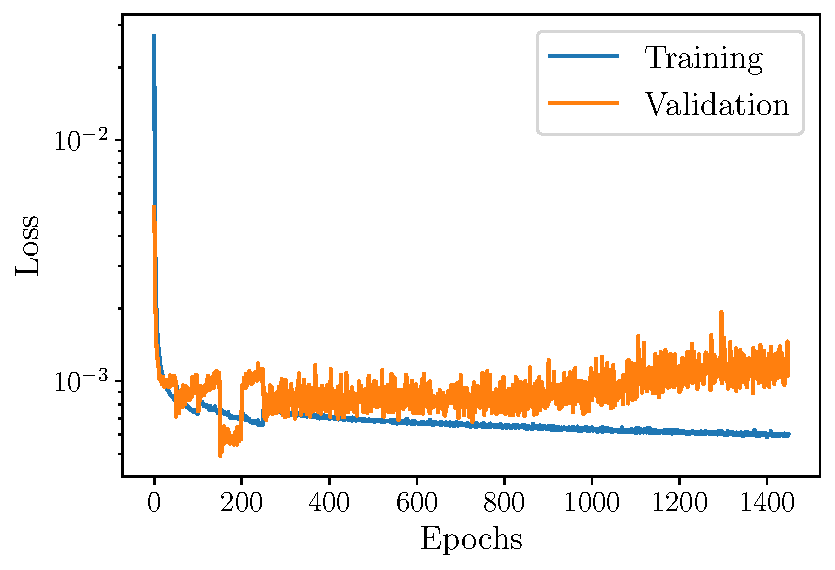
\includegraphics[width=\textwidth]{FNN_training_validation_loss}
	\end{subfigure}
	\caption{The training error and the validation error from the learning of an FNN model with increasing number of training iterations (epochs). }\label{fig-nn-fnn3}
\end{figure}


\subsubsection{FNN model} A summary of the FNN model used to train the datasets is presented in Table \ref{tab_fnn}. The input layer accepts the three features of the right stretch tensor and the output layer corresponds to the components of the $ 2^\text{nd} $-Piola Kirchhoff stress tensor for which the FNN needs to be trained, as presented in Eqs. (\ref{eq-nn-data3}) and (\ref{eq-nn-data4}). 

The datasets correspond to around 200000 independent stress-strain states for which the FNN model can be trained. The mean square error obtained by the training and the validation datasets are illustrated in Figure \ref{fig-nn-fnn3}. The training datasets correspond to the actual data that is used to update the model parameters $ \textbf{W}^S_{FNN} $ and as such with further training the error reduces, but whether the model generalizes for any data having a similar distribution as the training dataset can be visualized by validating the model using the validation dataset. The figure shows that the validation error stops reducing after some epochs and in fact starts showing the behavior of an overfitted model as it can not generalize any further for the given distribution of datasets.

\red{To avoid the use of overfitted models and predict poor results, here a choice to perform ``manual'' saving of the model at certain frequencies of epochs was made. This enables a higher degree of autonomy over the overall process. Also, one can compare the results between a well fit model and one that overfits with access to the entire range of saved features. It is also possible that the model training plateaus for reasons like appearance of a local minima or repeated initialization of random internal parameters leading in the opposite direction of the gradient curve. Forcing the model training process to continue with new batch of training data gives the user a better view of the model performance over new batches of data and differing hyperparameter values. However, using Keras API, one can choose to perform certain callback options where the model automatically performs the command, such as saving the model if validation error increases over a range of epochs that are predefined. It is also possible to terminate the training completely when the model notices a lack of improvement in model parameters over a range of epochs.}

\subsubsection{FNN Predictions}
To test the predictability of the FNN model, a set of new strain states, that were not part of the training or the validation datasets, were fed to the FNN. The results of this prediction test are presented in Figure \ref{fig-nn-fnn4}. For comparison, the results from the DNS simulations are also presented. 

\begin{figure}
	\centering
	\begin{subfigure}[t]{0.45\textwidth}
		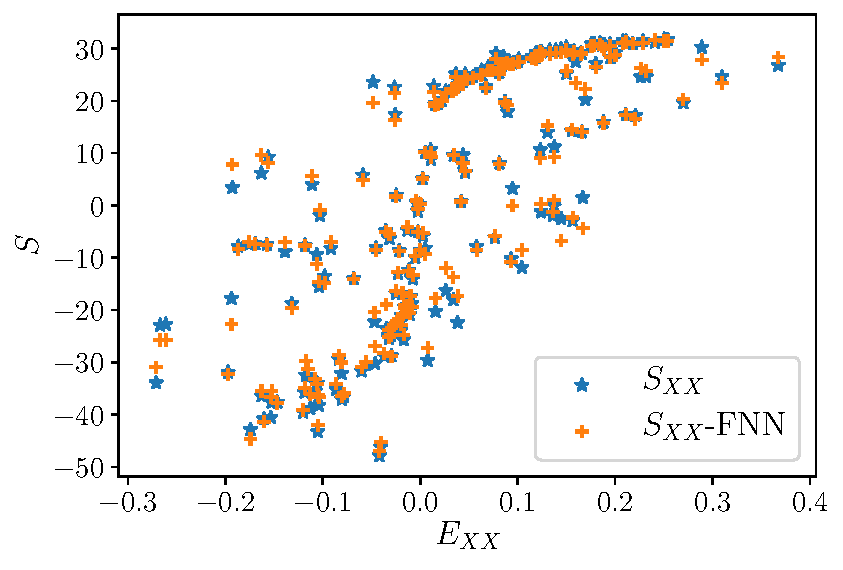
\includegraphics[width=\textwidth]{FNN_random_predict_0}
	\end{subfigure}
	\begin{subfigure}[t]{0.45\textwidth}
	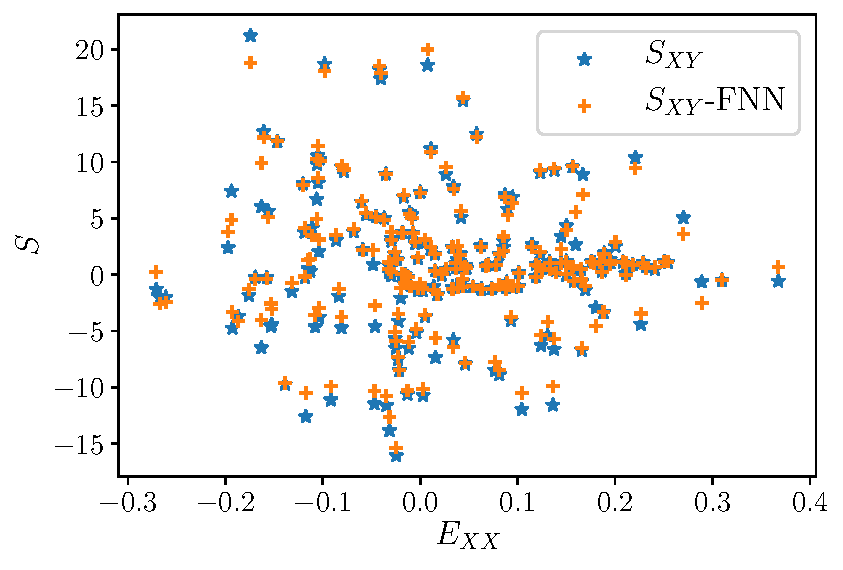
\includegraphics[width=\textwidth]{FNN_random_predict_1}
	\end{subfigure}
	\begin{subfigure}[t]{0.45\textwidth}
	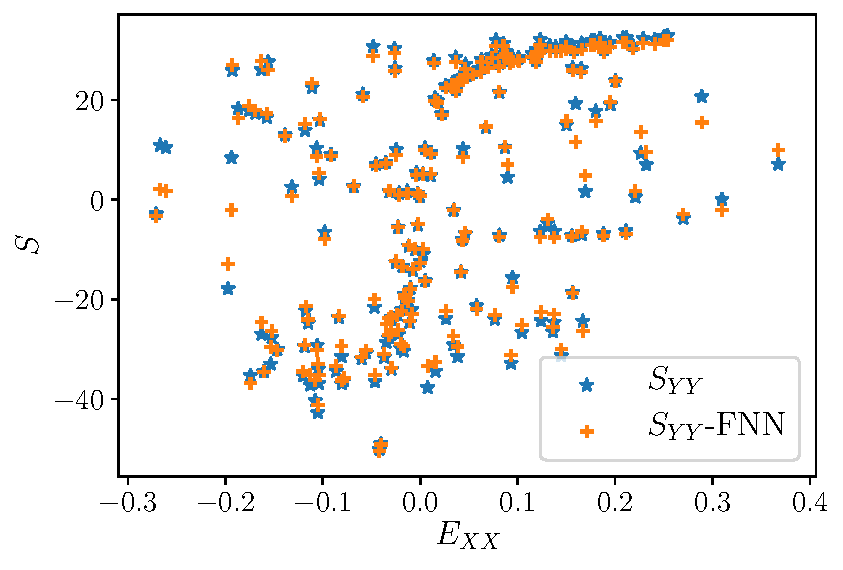
\includegraphics[width=\textwidth]{FNN_random_predict_3}
	\end{subfigure}
	\begin{subfigure}[t]{0.45\textwidth}
	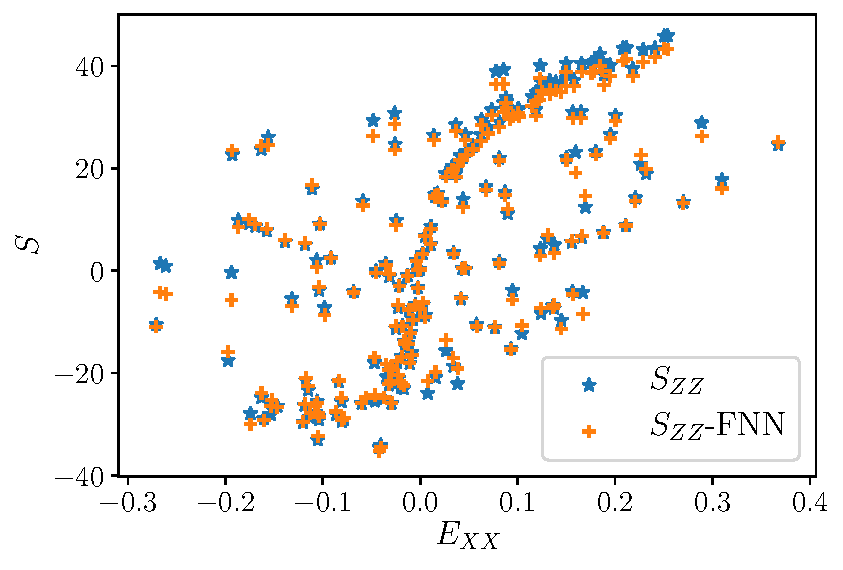
\includegraphics[width=\textwidth]{FNN_random_predict_4}
	\end{subfigure}
	\caption{Comparison between the DNS results and the FNN predictions of the stress (in MPa) for randomly selected strain states.}\label{fig-nn-fnn4}
\end{figure}

It is very evident that the predictability of an FNN for the case of proportional loading behavior in a material is quite good. This is especially true for data that is well within the bounds of the training dataset. At the outliers, one can see that there is a higher error in the prediction of the stress which can be easily explained as a result of insufficient training in and around that particular domain of the strain space.

\begin{figure}
	\centering
	\begin{subfigure}[t]{0.45\textwidth}
		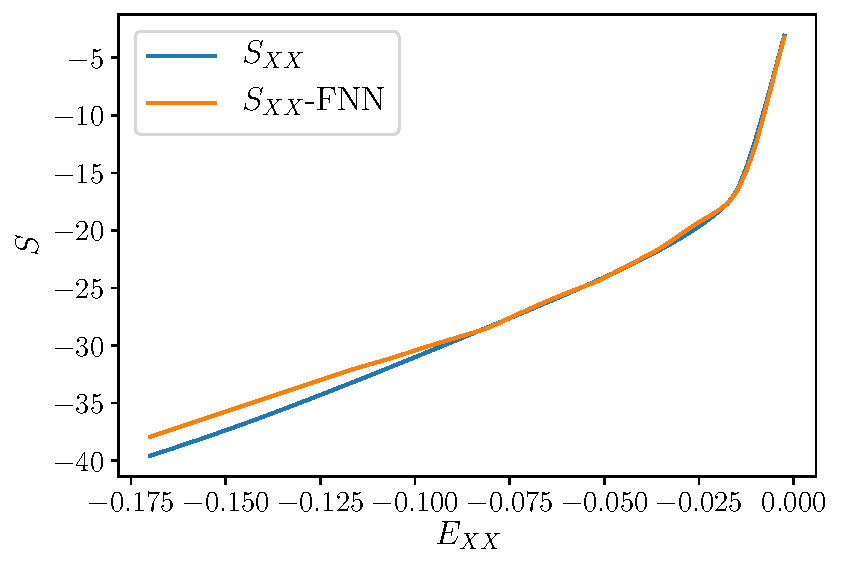
\includegraphics[width=\textwidth]{FNN_predict_uniaxial_0}
	\end{subfigure}
	\begin{subfigure}[t]{0.45\textwidth}
		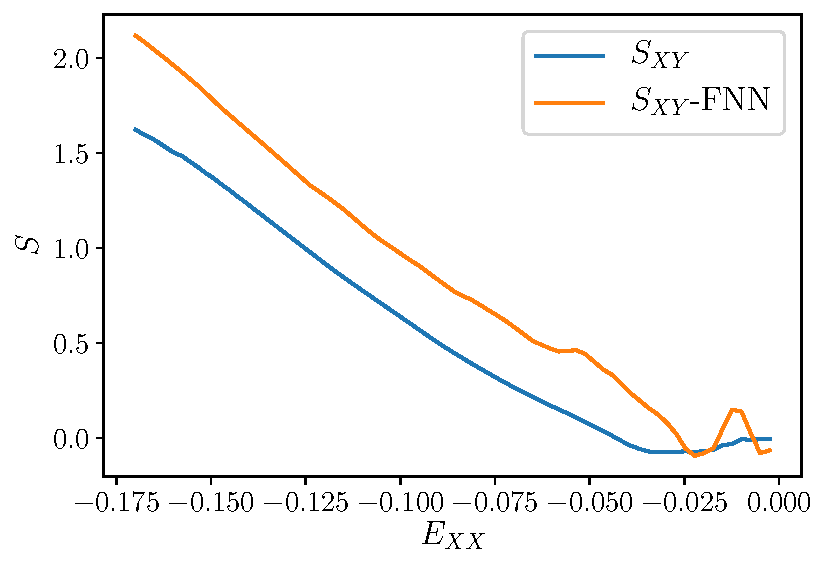
\includegraphics[width=\textwidth]{FNN_predict_uniaxial_1}
	\end{subfigure}
	\begin{subfigure}[t]{0.45\textwidth}
		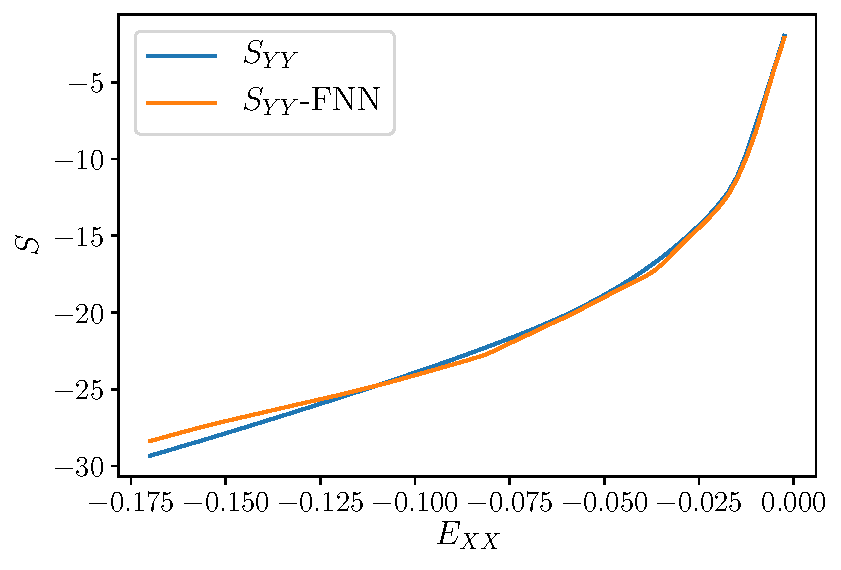
\includegraphics[width=\textwidth]{FNN_predict_uniaxial_3}
	\end{subfigure}
	\begin{subfigure}[t]{0.45\textwidth}
		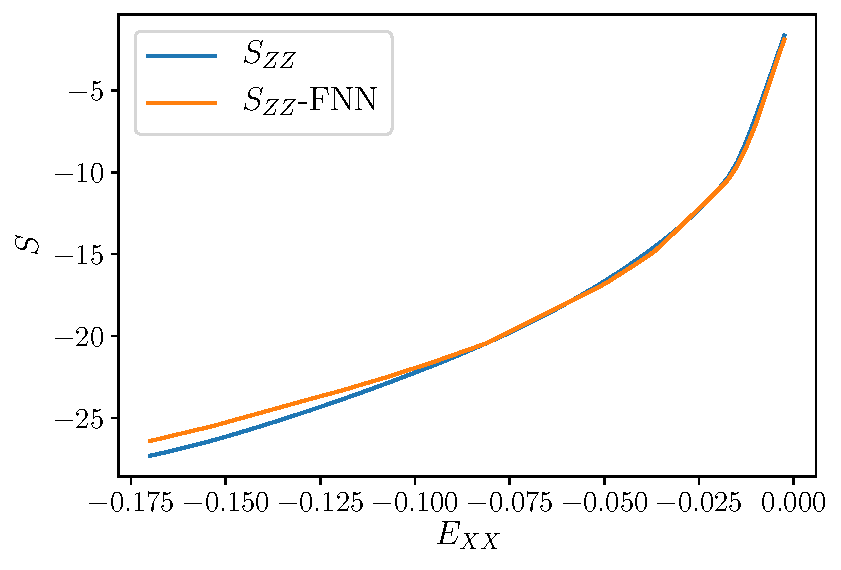
\includegraphics[width=\textwidth]{FNN_predict_uniaxial_4}
	\end{subfigure}
	\caption{Comparison of the stress (in MPa) predicted by the FNN model with that computed by a DNS analysis for a plane-strain compression test.}\label{fig-nn-fnn5-1}
\end{figure}

Figure \ref{fig-nn-fnn5-1} presents the results of the comparison between the FNN prediction and a DNS simulation results of the stress behavior of the material under a simple plane-strain compression load (non-zero $ {\tgm{E}}_{XX} $ and $ {\tgm{E}}_{YY}={\tgm{E}}_{ZZ}=0 $) with a good convergence between the two sets of results. (One could say that the values have sensitive fluctuations though, as can be observed for the behavior of $ S_{XY} $. It is possible that the values could converge by training further simulations, but in this case it was found that the model predictions did not improve further.)

\begin{figure}
	\centering
	\begin{subfigure}[t]{0.45\textwidth}
		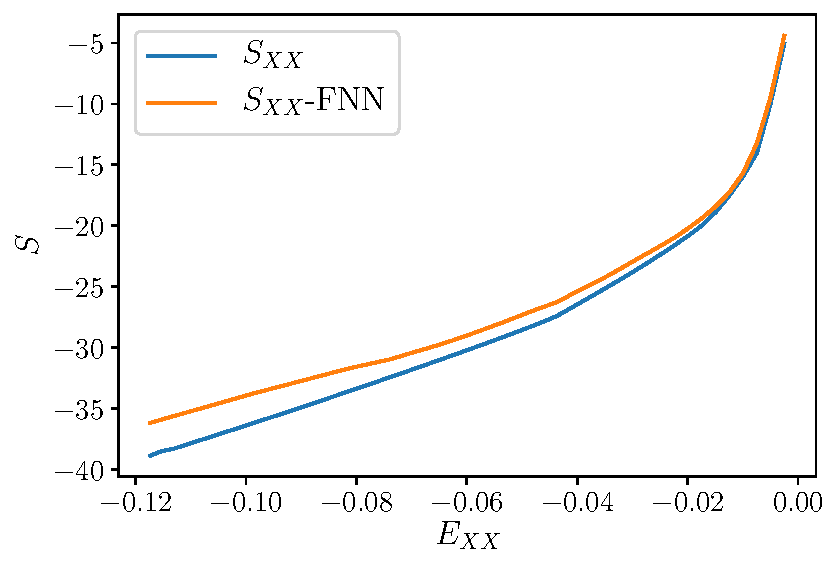
\includegraphics[width=\textwidth]{FNN_predict_Big4_0}
	\end{subfigure}
	\begin{subfigure}[t]{0.45\textwidth}
		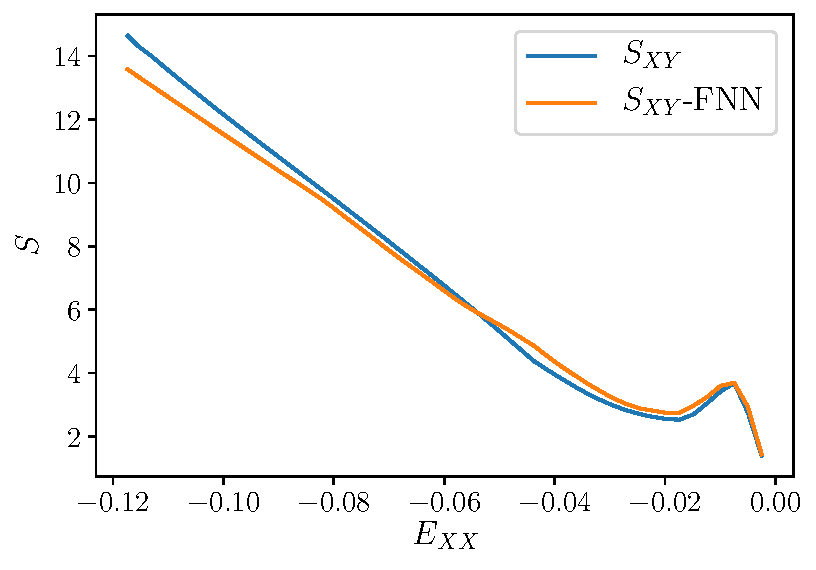
\includegraphics[width=\textwidth]{FNN_predict_Big4_1}
	\end{subfigure}
	\begin{subfigure}[t]{0.45\textwidth}
		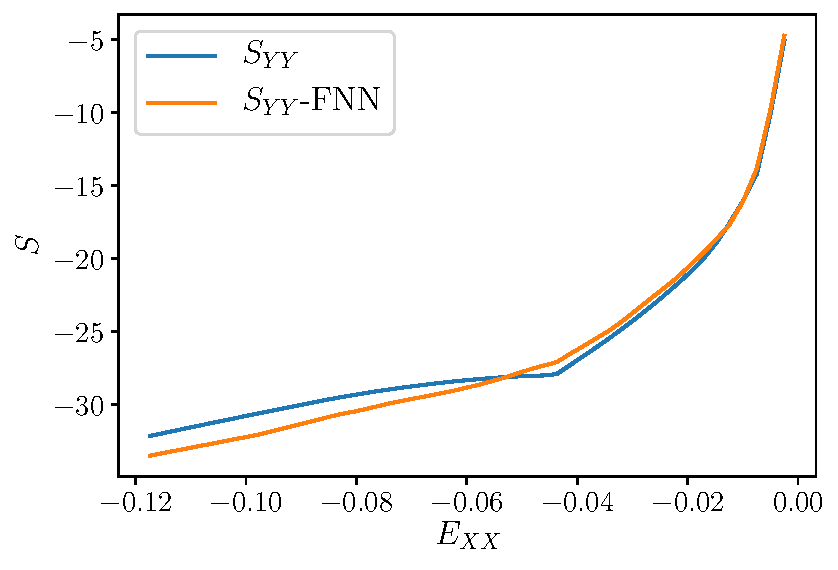
\includegraphics[width=\textwidth]{FNN_predict_Big4_3}
	\end{subfigure}
	\begin{subfigure}[t]{0.45\textwidth}
		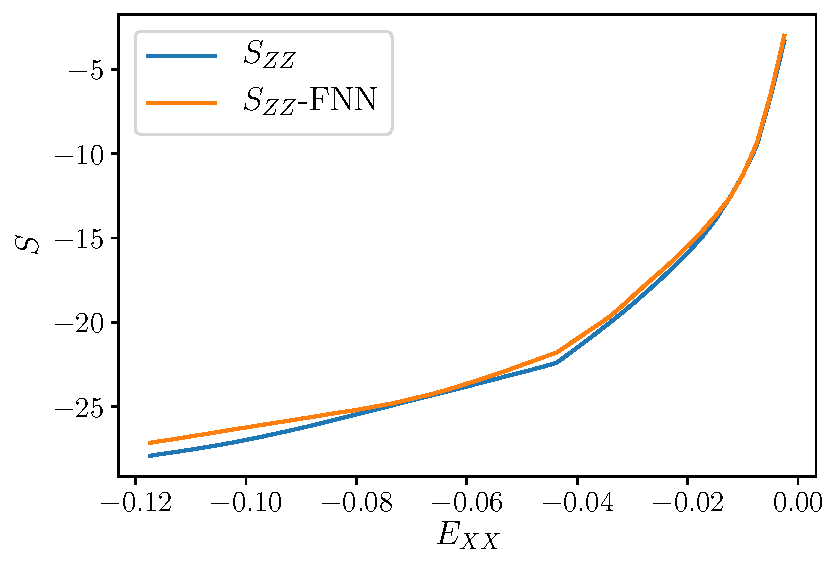
\includegraphics[width=\textwidth]{FNN_predict_Big4_4}
	\end{subfigure}
	\caption{Comparison of the stress (in MPa) predicted by the FNN model with that computed by a DNS analysis for a sequence of strain-states to show the ability of the FNN to work in an online computation as an efficient surrogate for monotonic proportional loading.}\label{fig-nn-fnn5}
\end{figure}

To plug the FNN as a surrogate for the micro-scale BVP in an \fee analysis, the FNN must have the ability to predict the real-time behavior of the material and then return the predictions back to the macroscopic BVP. A simple test of this ability can be done by simply feeding the strain-states in a sequential manner and then extracting back the predicted stress states. Figure \ref{fig-nn-fnn5} illustrates a comparison between the behavior observed in DNS results and from the predictions of the trained FNN for a random sequence of proportional loading.

\subsubsection{Computation cost}
\red{When a discussion on a data-driven surrogate takes place, it becomes a necessity to compare the cost of computation and present a comparison between the approaches used. In the current scenario, the preparation of datasets takes place at the rate of 5 simulations per hour per processor on a $ 6^\text{th} $-gen Intel-i7 processor assuming that each simulation converges till the predefined loading limit. So, for 3000 simulations, this comes at around 150 hours with 4 processors. Further, the training of the FNN model consumes around 2 hours to obtain an error rate less than $ 5\times10^{-4} $ with 4 processors.  This means that the implementation of an FNN surrogate breaks even after around 3040 simulations as the online prediction is an operation that consumes few seconds. The training time can be drastically reduced by running hundreds of simulations in parallel on clusters.} 

\subsection{Discussions on FNN surrogates}\label{nn-mono-discussion}
In this section, a proportional loading based training of an FNN model has been presented. By looking at the results, it is safe to conclude that the independent stress-strain states presented by the proportional loading is not a challenge for a simple FNN model. The proposed model does not need to be a deep network with many layers, because there is then the possibility of the model ``learning'' the data rather than ``generalizing'' from it due to the simplicity of the training datasets. A shallow network with sufficient neurons in each layer can easily learn from the data.

This study enables one to progress further with history dependent loading behavior where the stress-strain states are further strengthened with the internal state variables to obtain a complete representation of independent states of the material to predict the stress behavior of the material at any given loading point of the history dependent process.

This study also displays the ability to use ANN models to study mechanical behavior and sets up the premise for implementing complex ANN models like an LSTM or a GRU based RNN models simply by replacing one of the layers in the FNN model.


\section{History Dependent Behavior}\label{nn-dnn}

In the second case of study, two ways to predict history dependent material behavior are presented, one based on RNNs that uses LSTMs or GRUs and another made of two FNNs called \fnn model. This study is heavily influenced by the work done in \cite{wuRecurrentNeuralNetworkaccelerated2020} where a GRU based RNN has been used to study history dependent behavior. Random path based loading sequences as proposed in Section \ref{nn-gendata-rand} are used to generate training datasets which will be used to train and optimize the parameters of the two ANNs that are being proposed. 

Typically, for RNNs, stacks of the entire simulation sequences starting from the initial position can be introduced in batches as the model inputs so that the models can understand the history dependency and appropriately update the internal weights and bias vectors. The training datasets have to be prepared accordingly to be trained with an RNN based model.

In the case of \fnn models, the two component FNN models, further called \mbox{FNN-1} and \mbox{FNN-2}, can be trained independently. These are standard FNN models that work very similar to the ones proposed in Section \ref{nn-mono}, but composed of larger number of neurons to accommodate  the excess parameters introduced by the implementation of state variables. \mbox{FNN-1} is trained to predict the incremental state variables by taking in the incremental strain state along with the current state variables. \mbox{FNN-2} is trained to predict the resultant stress by looking at the state variables and the strain state. For this purpose, the data has to be prepared accordingly.

In this section, history dependent loading paths as described in Section \ref{nn-gendata} will be studied with RNNs and \fnn. The training datasets will be suitably prepared for this purpose and the link between the surrogates and the corresponding constituent law in an \fee method will be outlined. The usage of the RNN based models and the \fnn based models as surrogates will be detailed before presenting some results and discussing the aspects of this approach.

\subsection{Preparation of datasets for RNN}\label{nn-dnn-dataprep}

Recalling from Eqs. (\ref{eq-nn-data1}) and (\ref{eq-nn-data2}), the output of the FEM simulation can be obtained in a sequential manner. The RNN training data needs to be arranged in a sequential format so that the history of the data is carried forward along with the increase in time step. RNN training is more effective when large numbers of batches are trained together so that the weights do not get reset by small marginal variations. However, it is quite possible that for a particular training sequence the micro-scale BVP resolution does not converge before reaching the critical $ R_\text{max} $ or the predefined number of steps. Besides, since the increments are generated randomly, the sequences do not necessarily have the same length. To ensure an efficient training, a group of training sequences can be stacked together and ensured that they have the same length sequence by trimming and padding.

By padding, one can ensure that shorter training sequences are brought to the necessary length by either padding zeros before the first value of the sequence, or by padding the end of the sequence by the last value of the sequence until the length of the sequence matches the global average sequence length of the batch in training. By trimming, one can snip off elements that fall beyond the predefined sequence length, so that the batch training is not unnecessarily dragged for one stray sequence. 

{Padding and trimming have been summarized in Table \ref{tab_padding} for a sequence of values $ \textbf{X} $ made of individual elements $ \mathcal{X}_i $ for a desired sequence length $ N_S $.}

\begin{table}
	\begin{tabular}{|>{\raggedright\arraybackslash}p{0.15\textwidth}|p{0.4\textwidth}|p{0.4\textwidth}|}
\hline
\rule{0pt}{4ex}    
Padding with zeros & \raggedright\arraybackslash$ \textbf{X}_0^{N_S-2}$$=$$\left[\mathcal{X}_1,\mathcal{X}_2,\mathcal{X}_3,...,\mathcal{X}_{N_S-2}\right] $ & \raggedright\arraybackslash$ \textbf{X}_0^{N_S}$$=$$\left[0,0,\mathcal{X}_1,...,\mathcal{X}_{N_S-2}\right] $\\ 
\hline 
\rule{0pt}{4ex}    
Padding with last value & \raggedright\arraybackslash$ \textbf{X}_0^{N_S-2}$$=$$\left[\mathcal{X}_1,\mathcal{X}_2,\mathcal{X}_3,...,\mathcal{X}_{N_S-2}\right] $ & \raggedright\arraybackslash$ \textbf{X}_0^{N_S}$$=$$\left[\mathcal{X}_1,...,\mathcal{X}_{N_S-2},\mathcal{X}_{N_S-2},\mathcal{X}_{N_S-2}\right] $\\ 
\hline 
\rule{0pt}{4ex}    
Trimming sequences & \raggedright\arraybackslash$ \textbf{X}_0^{N_S+2}$$=$$\left[\mathcal{X}_1,...,\mathcal{X}_{N_S},\mathcal{X}_{N_S+1},\mathcal{X}_{N_S+2}\right] $ & \raggedright\arraybackslash$ \textbf{X}_0^{N_S}$$=$$\left[\mathcal{X}_1,...,\mathcal{X}_{N_S}\right],$\sout{$\mathcal{X}_{N_S+1}$},\sout{$\mathcal{X}_{N_S+2}$} \\ 
\hline
	\end{tabular}
\caption{Summary of padding and trimming of sequences for RNN training.}\label{tab_padding}
\end{table}

With the goal of having a predefined number of steps in each sequence, one can obtain the requisite input and output for the RNNs in terms of the right stretch strain tensor $ \tgm[]{E} $ and 2$ ^\text{nd} $-Piola-Kirchhoff stress tensor $ \tgm[]{S} $, respectively, as
\begin{eqnarray}\label{eq-nn-data5}
\tgm[]{E}^{RNN}=
\left[\begin{array}{c}
...\\\tgm[]{E}^{i-1}\\\tgm[]{E}^i\\\tgm[]{E}^{i+1}\\...
\end{array}\right]
=
\left[\begin{array}{c c c c}
& & ... & \\
{\tgm[]{E}^{i-1}}_0 & {\tgm[]{E}^{i-1}}_1 & ... & {\tgm[]{E}^{i-1}}_{N_S}\\
{\tgm[]{E}^{i}}_0 & {\tgm[]{E}^{i}}_1 & ... & {\tgm[]{E}^{i}}_{N_S}\\
{\tgm[]{E}^{i+1}}_0 & {\tgm[]{E}^{i+1}}_1 & ... & {\tgm[]{E}^{i+1}}_{N_S}\\
& & ... &
\end{array}\right]
\end{eqnarray}
\begin{eqnarray}\label{eq-nn-data6}
\tgm[]{S}^{RNN}=
\left[\begin{array}{c}
...\\\tgm[]{S}^{i-1}\\\tgm[]{S}^i\\\tgm[]{S}^{i+1}\\...
\end{array}\right]
=
\left[\begin{array}{c c c c}
& & ... & \\
{\tgm[]{S}^{i-1}}_0 & {\tgm[]{S}^{i-1}}_1 & ... & {\tgm[]{S}^{i-1}}_{N_S}\\
{\tgm[]{S}^{i}}_0 & {\tgm[]{S}^{i}}_1 & ... & {\tgm[]{S}^{i}}_{N_S}\\
{\tgm[]{S}^{i+1}}_0 & {\tgm[]{S}^{i+1}}_1 & ... & {\tgm[]{S}^{i+1}}_{N_S}\\
& & ... &
\end{array}\right]
\end{eqnarray}
where $ i=1,..,N_{samples} $. The data is normalized using a min-max-scaler as the RNNs work more efficiently when the data is scaled and prepared well.

\subsection{Preparation of datasets for \fnn}
In the considered \fnn model, two FNNs are trained simultaneously. The data needed to train the two models have to be appropriately structured. Considering that a single FNN can not be used in a direct manner to replicate history dependent behavior, the concept of state-based representation presented in Section \ref{nn-dnn-state} and the concept of clustering presented in Section \ref{nn-dnn-scc} are used here to present a definitive state value that mimics the behavior of cell-state in RNN modules.

The analysis of the random strain path $ \tgm[]{U}^i $ gives information about the internal state $ \tgm[]{Z}^i $ and the stress tensor $ \tgm[]{P}^i $, as 
\begin{equation}\label{eq-nn-data7}
\tgm[]{Z}^i=\left[{\tgm[]{Z}^i}_0,{\tgm[]{Z}^i}_1,...,{\tgm[]{Z}^i}_{N_S}\right]
\end{equation}
\begin{equation}\label{eq-nn-data8}
\tgm[]{P}^i=\left[{\tgm[]{P}^i}_0,{\tgm[]{P}^i}_1,...,{\tgm[]{P}^i}_{N_S}\right].
\end{equation}
Between any two given time steps, $  \Delta t_{n+1}=t_{n+1}-t_n  $, the values of $ {\tgm[]{U}}_n^i $, $ {\tgm[]{U}}_{n+1}^i $ and $ {\tgm[]{Z}}_n^i $ are known. The values of $ \overset{.}{\textbf{Z}}_\text{M}^i $ needed in Eq. (\ref{eq-ch-state2}) and $ \overset{.}{\textbf{U}}_\text{M}^i $ needed in Eq. (\ref{eq-ch-state4}) approximated as 
\begin{equation}\label{eq-nn-data9}
\overset{.}{\textbf{Z}}_\text{M}^i=\frac{{\Delta\tgm[]{Z}}_{n+1}}{\Delta t_{n+1}}
\end{equation}
\begin{equation}\label{eq-nn-data10}
\overset{.}{\textbf{U}}_\text{M}^i=\frac{{\Delta\tgm[]{U}}_{n+1}}{\Delta t_{n+1}}
\end{equation}
where $ {\Delta\tgm[]{Z}}_{n+1}={\tgm[]{Z}}_{n+1}-{\tgm[]{Z}}_{n} $ and $ {\Delta\tgm[]{U}}_{n+1}={\tgm[]{U}}_{n+1}-{\tgm[]{U}}_{n} $. With this knowledge, the data necessary to train the \fnn model can be structured in a sequence for every training sample with the right stretch strain tensor $ \tgm[]{E} $, 2$ ^\text{nd} $-Piola-Krichhoff stress tensor $ \tgm[]{S} $, incremental right stretch strain tensor $ \Delta\tgm[]{E} $, internal state vector $ \tgm[]{Z} $, incremental internal state change vector $ \Delta\tgm[]{Z} $ as
\begin{eqnarray}\label{eq-nn-data12}
\tgm[]{E}^{FNN^2}=\left[..,\tgm[]{E}^{i-1},\tgm[]{E}^i,\tgm[]{E}^{i+1},..\right] = 
\left[..,{\tgm[]{E}^{i-1}}_0,{\tgm[]{E}^{i-1}}_1,...,{\tgm[]{E}^{i-1}}_{N_{s_{i-1}}},\right.\nonumber\\
{\tgm[]{E}^i}_0,{\tgm[]{E}^i}_1,...,{\tgm[]{E}^i}_{N_{s_i}},
\left.{\tgm[]{E}^{i+1}}_0,{\tgm[]{E}^{i+1}}_1,...,{\tgm[]{E}^{i+1}}_{N_{s_{i+1}}},..\right],
\end{eqnarray}
\begin{eqnarray}\label{eq-nn-data12-1}
\Delta\tgm[]{E}^{FNN^2}=\left[..,\Delta\tgm[]{E}^{i-1},\Delta\tgm[]{E}^i,\Delta\tgm[]{E}^{i+1},..\right] = 
\left[..,{\Delta\tgm[]{E}^{i-1}}_0,{\Delta\tgm[]{E}^{i-1}}_1,...,{\Delta\tgm[]{E}^{i-1}}_{N_{s_{i-1}}},\right.\nonumber\\
{\Delta\tgm[]{E}^i}_0,{\Delta\tgm[]{E}^i}_1,...,{\Delta\tgm[]{E}^i}_{N_{s_i}},
\left.{\Delta\tgm[]{E}^{i+1}}_0,{\Delta\tgm[]{E}^{i+1}}_1,...,{\Delta\tgm[]{E}^{i+1}}_{N_{s_{i+1}}},..\right],
\end{eqnarray}
\begin{eqnarray}\label{eq-nn-data13}
\tgm[]{S}^{FNN^2}=\left[..,\tgm[]{S}^{i-1},\tgm[]{S}^i,\tgm[]{S}^{i+1},..\right] = 
\left[..,{\tgm[]{S}^{i-1}}_0,{\tgm[]{S}^{i-1}}_1,...,{\tgm[]{S}^{i-1}}_{N_{s_{i-1}}},\right.\nonumber\\
{\tgm[]{S}^i}_0,{\tgm[]{S}^i}_1,...,{\tgm[]{S}^i}_{N_{s_i}},
\left.{\tgm[]{S}^{i+1}}_0,{\tgm[]{S}^{i+1}}_1,...,{\tgm[]{S}^{i+1}}_{N_{s_{i+1}}},..\right],
\end{eqnarray}
\begin{eqnarray}\label{eq-nn-data14}
\tgm[]{Z}^{FNN^2}=\left[..,\tgm[]{Z}^{i-1},\tgm[]{Z}^i,\tgm[]{Z}^{i+1},..\right] = 
\left[..,{\tgm[]{Z}^{i-1}}_0,{\tgm[]{Z}^{i-1}}_1,...,{\tgm[]{Z}^{i-1}}_{N_{s_{i-1}}},\right.\nonumber\\
{\tgm[]{Z}^i}_0,{\tgm[]{Z}^i}_1,...,{\tgm[]{Z}^i}_{N_{s_i}},
\left.{\tgm[]{Z}^{i+1}}_0,{\tgm[]{Z}^{i+1}}_1,...,{\tgm[]{Z}^{i+1}}_{N_{s_{i+1}}},..\right],
\end{eqnarray}
\begin{eqnarray}\label{eq-nn-data15}
\Delta\tgm[]{Z}^{FNN^2}=\left[..,\Delta\tgm[]{Z}^{i-1},\Delta\tgm[]{Z}^i,\Delta\tgm[]{Z}^{i+1},..\right] = 
\left[..,{\Delta\tgm[]{Z}^{i-1}}_0,{\Delta\tgm[]{Z}^{i-1}}_1,...,{\Delta\tgm[]{Z}^{i-1}}_{N_{s_{i-1}}},\right.\nonumber\\
{\Delta\tgm[]{Z}^i}_0,{\Delta\tgm[]{Z}^i}_1,...,{\Delta\tgm[]{Z}^i}_{N_{s_i}},
\left.{\Delta\tgm[]{Z}^{i+1}}_0,{\Delta\tgm[]{Z}^{i+1}}_1,...,{\Delta\tgm[]{Z}^{i+1}}_{N_{s_{i+1}}},..\right],
\end{eqnarray}

\subsection{Material Law with RNN}\label{nn-dnn-material}
The idea behind using an RNN based model as a surrogate for the micro-scale BVP is comparable to the implementation of an FNN in the study of monotonic proportional loading behavior. In the case of the study of history dependent behavior with RNNs, Eq. (\ref{eq-nn-law1}) can be written as
\begin{equation}\label{eq-nn-law3}
{\tgm[]{S}}^{RNN} = \mathcal{S}^{RNN}({\tgm[]{E}}^{RNN};\textbf{W}^S_{RNN})
\end{equation}
where $ \mathcal{S}^{RNN} $ is the RNN network that corresponds to the surrogate and $ \textbf{W}^S_{RNN} $ are the trainable parameters of the network. Once optimized, $ \textbf{W}^S_{RNN} $ and the resultant $ \mathcal{S}^{RNN} $ can be used to predict the stress sequence $ \tgm{S}^{RNN} $ of a material under random path loading for any given strain sequence $ \tgm{E}^{RNN} $. Eq. (\ref{eq-nn-law3}) is analogous to Eq. (\ref{eq-nn-func}) that presents a global ANN system with the input $ \textbf{\textit{u}}=\tgm[]{E}^{RNN} $ and the output $ \textbf{\textit{v}}=\tgm[]{S}^{RNN} $.

\subsection{Material Law with \fnn}\label{nn-fnn2-material}
The proposed \fnn model is expected to serve dual purpose, one as a surrogate that can predict the stress state of a material under history dependent loading, and the other as a surrogate that can generate the state variable necessary to continue the micro-scale BVP analysis in a standard \fee computation. The data from the two component FNNs, \mbox{FNN-1} and \mbox{FNN-2}, have to be linked appropriately so that this dual purpose is achieved.

Following on from the material law that was presented in Eqs. (\ref{eq-ch-state2}) and (\ref{eq-ch-state4}), one can idealize this model using \fnn as
\begin{equation}\label{eq-nn-law4}
\Delta{\tgm[]{Z}}^{FNN^2}_{t+1}=\mathcal{Z}^{FNN^2}\left({\tgm[]{E}}^{FNN^2}_t,\Delta{\tgm[]{E}}^{FNN^2}_{t+1},{\tgm[]{Z}}^{FNN^2}_t;\textbf{W}^Z\right)
\end{equation}
\begin{equation}\label{eq-nn-law5}
{\tgm[]{Z}}^{FNN^2}_{t+1}={\tgm[]{Z}}^{FNN^2}_{t}+\Delta{\tgm[]{Z}}^{FNN^2}_{t+1}
\end{equation}
\begin{equation}\label{eq-nn-law6}
{\tgm[]{S}}^{FNN^2}_{t+1}=\mathcal{S}^{FNN^2}\left({\tgm[]{E}}^{FNN^2}_{t+1},{\tgm[]{Z}}^{FNN^2}_{t+1};\textbf{W}^S\right)
\end{equation}
where $ \mathcal{Z}^{FNN^2} $ and $ \mathcal{S}^{FNN^2} $ represent the \mbox{FNN-1} and \mbox{FNN-2} respectively that constitute the \fnn, and $ \textbf{W}^Z $ and $ \textbf{W}^S $ the corresponding parameters that need to be trained. Here Eq. (\ref{eq-nn-law4}) representing FNN-1 is analogous to ANN system represented in Eq. (\ref{eq-nn-func}) with the input $ \textbf{\textit{u}}=\{{\tgm[]{E}}^{FNN^2}_t,\Delta{\tgm[]{E}}^{FNN^2}_{t+1},{\tgm[]{Z}}^{FNN^2}_t\} $ and the output $ \textbf{\textit{v}}=\Delta{\tgm[]{Z}}^{FNN^2}_{t+1} $. Similarly, for FNN-2 represented by Eq. (\ref{eq-nn-law6}), $ \textbf{\textit{u}}=\{{\tgm[]{E}}^{FNN^2}_{t+1},{\tgm[]{Z}}^{FNN^2}_{t+1}\} $ and $ \textbf{\textit{v}}=\Delta{\tgm[]{Z}}^{FNN^2}_{t+1} $ represent the input and the output respectively.

\subsection{Online computation with trained RNN}\label{nn-dnn-online}
The online implementation of RNNs is very similar to that of an FNN as outlined in Section \ref{nn-mono-train}. The difference being that the entire strain sequence until the stage $ t $, where the prediction is needed, has to be provided to the RNN model. Following Eqs. (\ref{eq-fnn-1}) and (\ref{eq-fnn-2}), one can write the strain sequence as
\begin{equation}\label{eq-rnn-1}
{\tgm{E}}_T=\left[{\tgm{E}}_0,...,{\tgm{E}}_t\right].
\end{equation}
This ensures that the historical dependency of the material on the previous loading pattern can effectively influence the prediction of the RNN model. With the trained parameters $ \textbf{W}^S_{RNN} $, the predicted sequence can be obtained as
\begin{equation}\label{eq-rnn-2}
{\tgm{S}}_T^P=\mathcal{S}^{RNN}\left({\tgm{E}}_T;\textbf{W}^S_{RNN}\right),
\end{equation}
where 
\begin{equation}\label{eq-rnn-3}
{\tgm{S}}_T^P=\left[{\tgm{S}}_0^P,...,{\tgm{S}}_t^P\right],
\end{equation}
with $ {\tgm{S}}_t^P $ being the feature at stage $ t $. Eq. (\ref{eq-fnn-4}) can be recalled to obtain the necessary values.
 
\subsection{Online computation with trained \fnn}\label{nn-fnn2-online}
\fnn can be used online to obtain the incremental internal state vector at stage $ t+1 $ and the stress values at stage $ t+1 $. Since the components of \fnn are simple FNN models, the variables at a single stage are sufficient to compute the predicted values.

Recalling Eqs. (\ref{eq-fnn-1}) and (\ref{eq-fnn-2}), one can obtain $ {\tgm{E}}_t $. Once this is available, the incremental strain can be obtained by,
\begin{equation}\label{eq-fnn2-1}
\Delta{\tgm{E}}_{t+1}={\tgm{E}}_{t+1}-{\tgm{E}}_{t}.
\end{equation}
The state variables $ {\tgm{Z}}_t $ are available through the BVP solution of the micro-scale at stage $ t $. With the trained paramters, $ \textbf{W}^Z $, one can then predict the incremental state variable as
\begin{equation}\label{eq-fnn2-2}
\Delta{\tgm{Z}}_{t+1}^P=\mathcal{Z}^{FNN^2}\left({\tgm{E}}_t,\Delta{\tgm{E}}_{t+1},{\tgm{Z}}_t;\textbf{W}^Z\right).
\end{equation}
The internal state can be updated by
\begin{equation}\label{eq-fnn2-3}
{\tgm{Z}}_{t+1}^P={\tgm{Z}}_t+\Delta{\tgm{Z}}_{t+1}^P.
\end{equation}
This predicted state variable can be then used by FNN-2 with its trained parameter $ \textbf{W}^S $ to predict the stress output as
\begin{equation}\label{eq-fnn2-4}
{\tgm{S}}_{t+1}^P=\mathcal{S}^{FNN^2}\left({\tgm{E}}_{t+1},{\tgm{Z}}_{t+1}^P;\textbf{W}^S\right).
\end{equation} 
The 1$^\text{st} $-Piola Kirchhoff stress tensor can now be obtained using Eq. (\ref{eq-fnn-4}). The predicted state variable, $ {\tgm{Z}}^P_{t+1} $ along with $ {\tgm{E}}_{t+1} $ can be then used as the input of FNN-1 to obtain $ \Delta{\tgm{Z}}_{t+2}^P $ and so on to continue the chain of predictions.

\subsection{Verification of surrogates for history dependent analysis}
A set of random loading paths has been extracted and the material behavior have been recorded to be used as training and validation dataset for both RNN and \fnn models.

\begin{figure}
	\centering
	\begin{subfigure}{0.49\textwidth}
		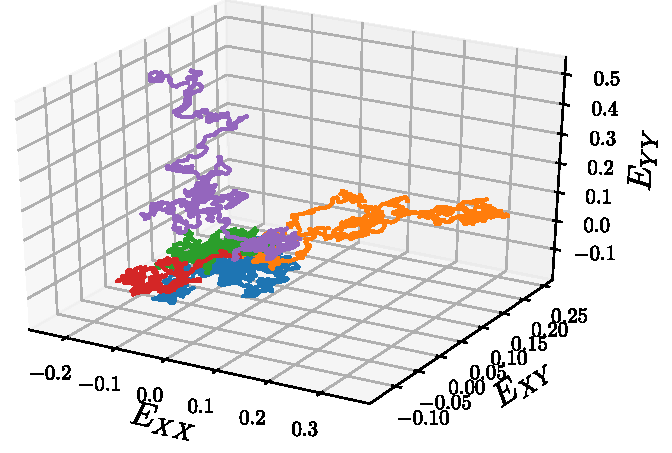
\includegraphics[width=\textwidth]{RNN_random_sequece}
		\caption{}
	\end{subfigure}
	\begin{subfigure}{0.49\textwidth}
		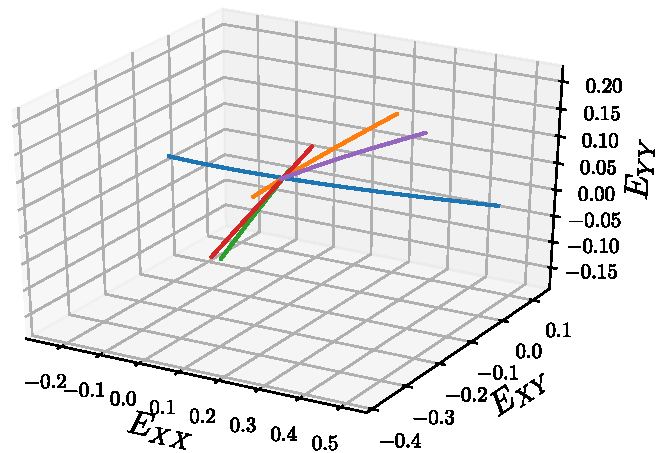
\includegraphics[width=\textwidth]{RNN_cyclic_sequece}
		\caption{}
	\end{subfigure}
	\caption{Some sample strain sequences generated by (a) the random path algorithm, and (b) random cyclic load algorithm, used to train the RNN and \fnn models. It is quite possible that a lot of the strain sequences get terminated prematurely during the DNS analysis due to the restriction of the number of times the time step can be reduced in case of convergence issues.}\label{fig-rnn-1}
\end{figure}

\subsubsection{Preparation of Datasets} The datasets consist of history dependent stress-strain states along with the corresponding internal state variables as described in Section \ref{nn-gendata-rand} and \ref{nn-dnn-state}. Both random cyclic loading and random path loading data were generated. A value of $ R_\text{max}=0.4 $ and $ \Delta R_\text{min}=0.0025 $ was provided so as to ensure that the domain of stress-strain states is covered to a good extent. To ensure long sequences of history dependent behavior, $ N_S=1000 $ was used. The generated data is such that the maximum and minimum bounds of the right stretch tensor are
\begin{eqnarray}\label{eq-rnn-res1}
\textbf{E}_\text{min}&=&\min\left(E_{XX}^{RNN},E_{XY}^{RNN},E_{YY}^{RNN}\right)\nonumber\\&=&\left[-0.35022, -0.52974, -0.38217\right]\nonumber
\end{eqnarray}
and
\begin{eqnarray}\label{eq-rnn-res2}
\textbf{E}_\text{max}&=&\max\left(E_{XX}^{RNN},E_{XY}^{RNN},E_{YY}^{RNN}\right)\nonumber\\&=&\left[0.87961, 0.70712, 0.94639\right].\nonumber
\end{eqnarray}

\begin{figure}
	\centering
	\begin{subfigure}[t]{0.45\textwidth}
		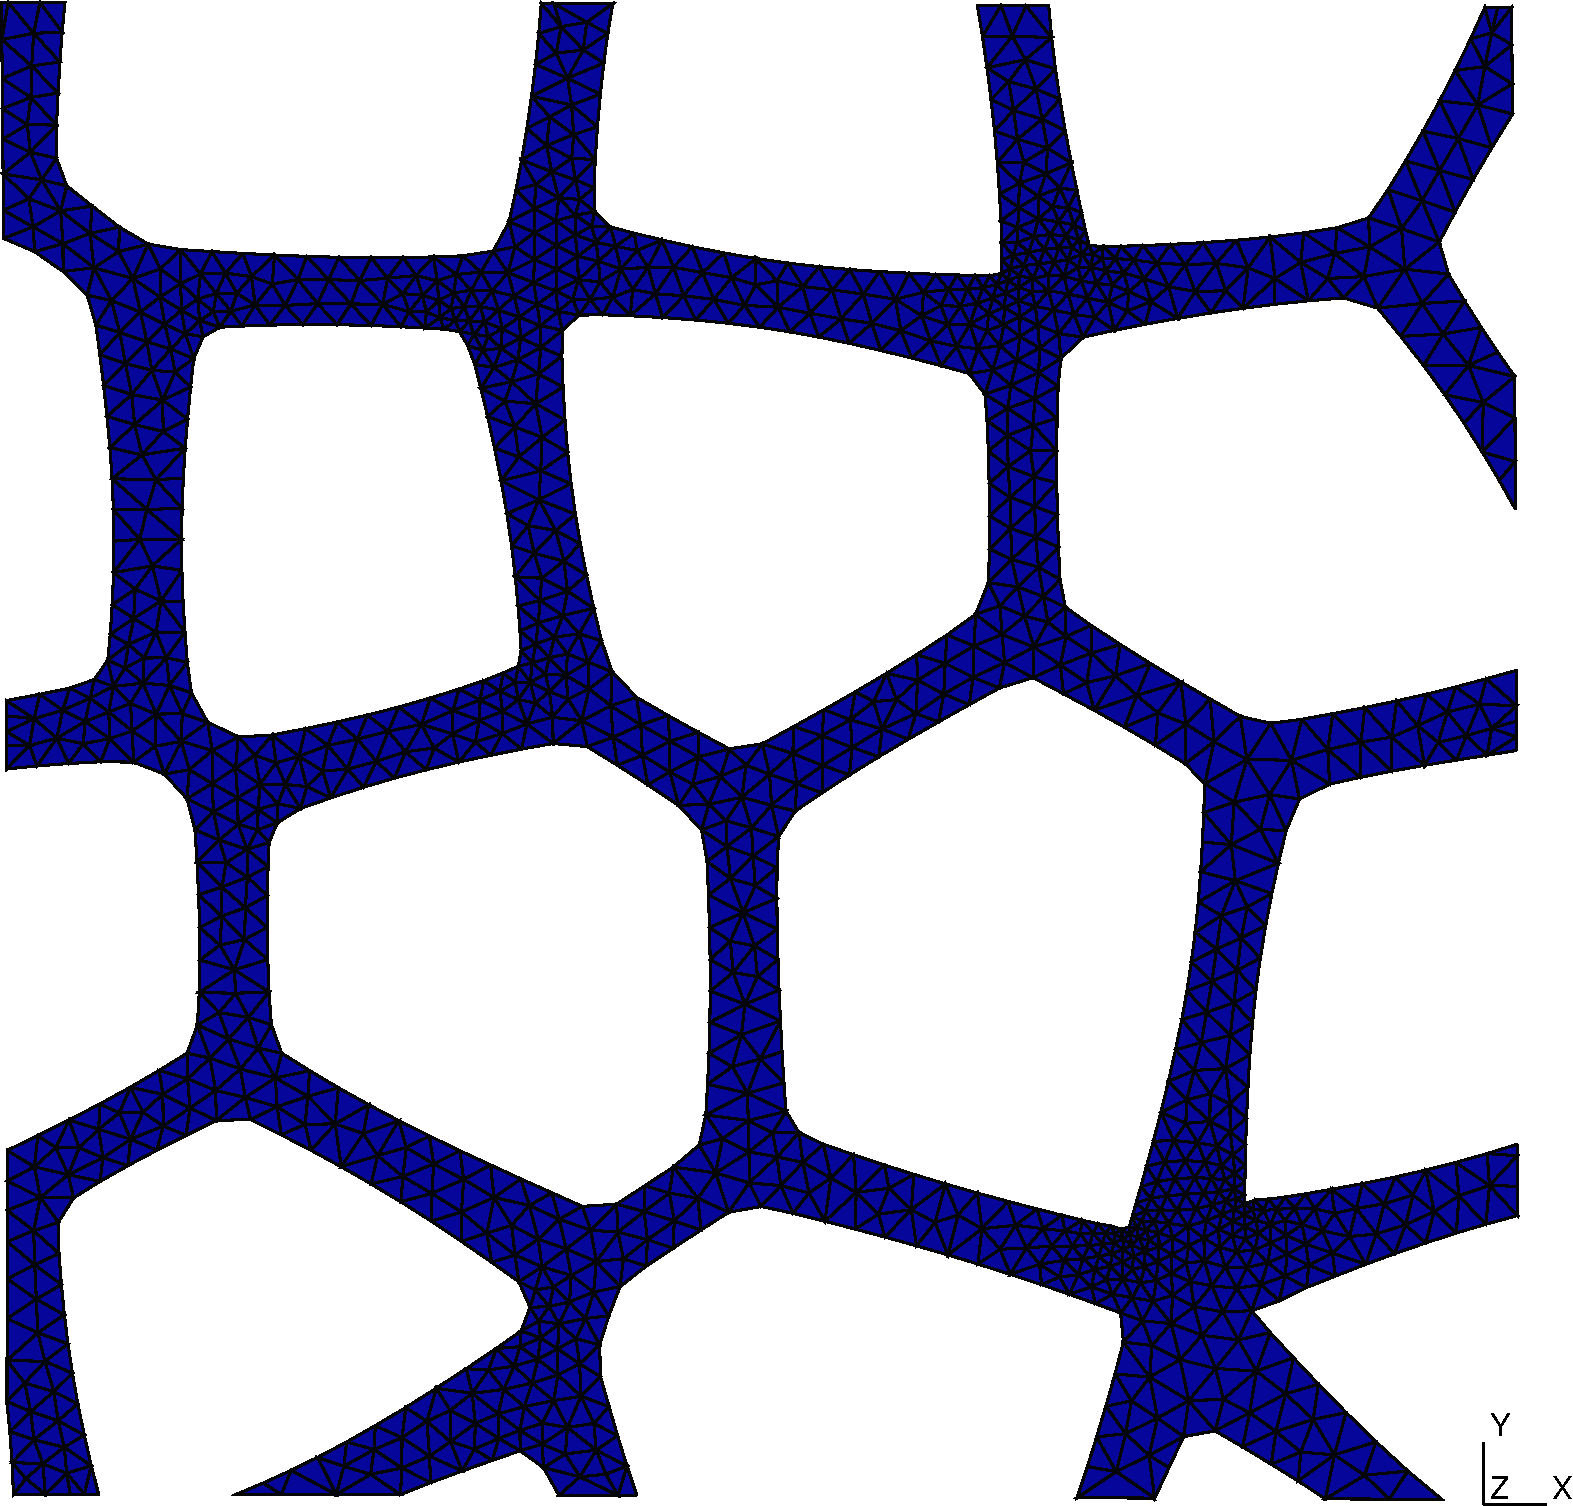
\includegraphics[height=4.cm]{eqps_1_1}
	\caption{}
	\end{subfigure}
	\begin{subfigure}[t]{0.45\textwidth}
		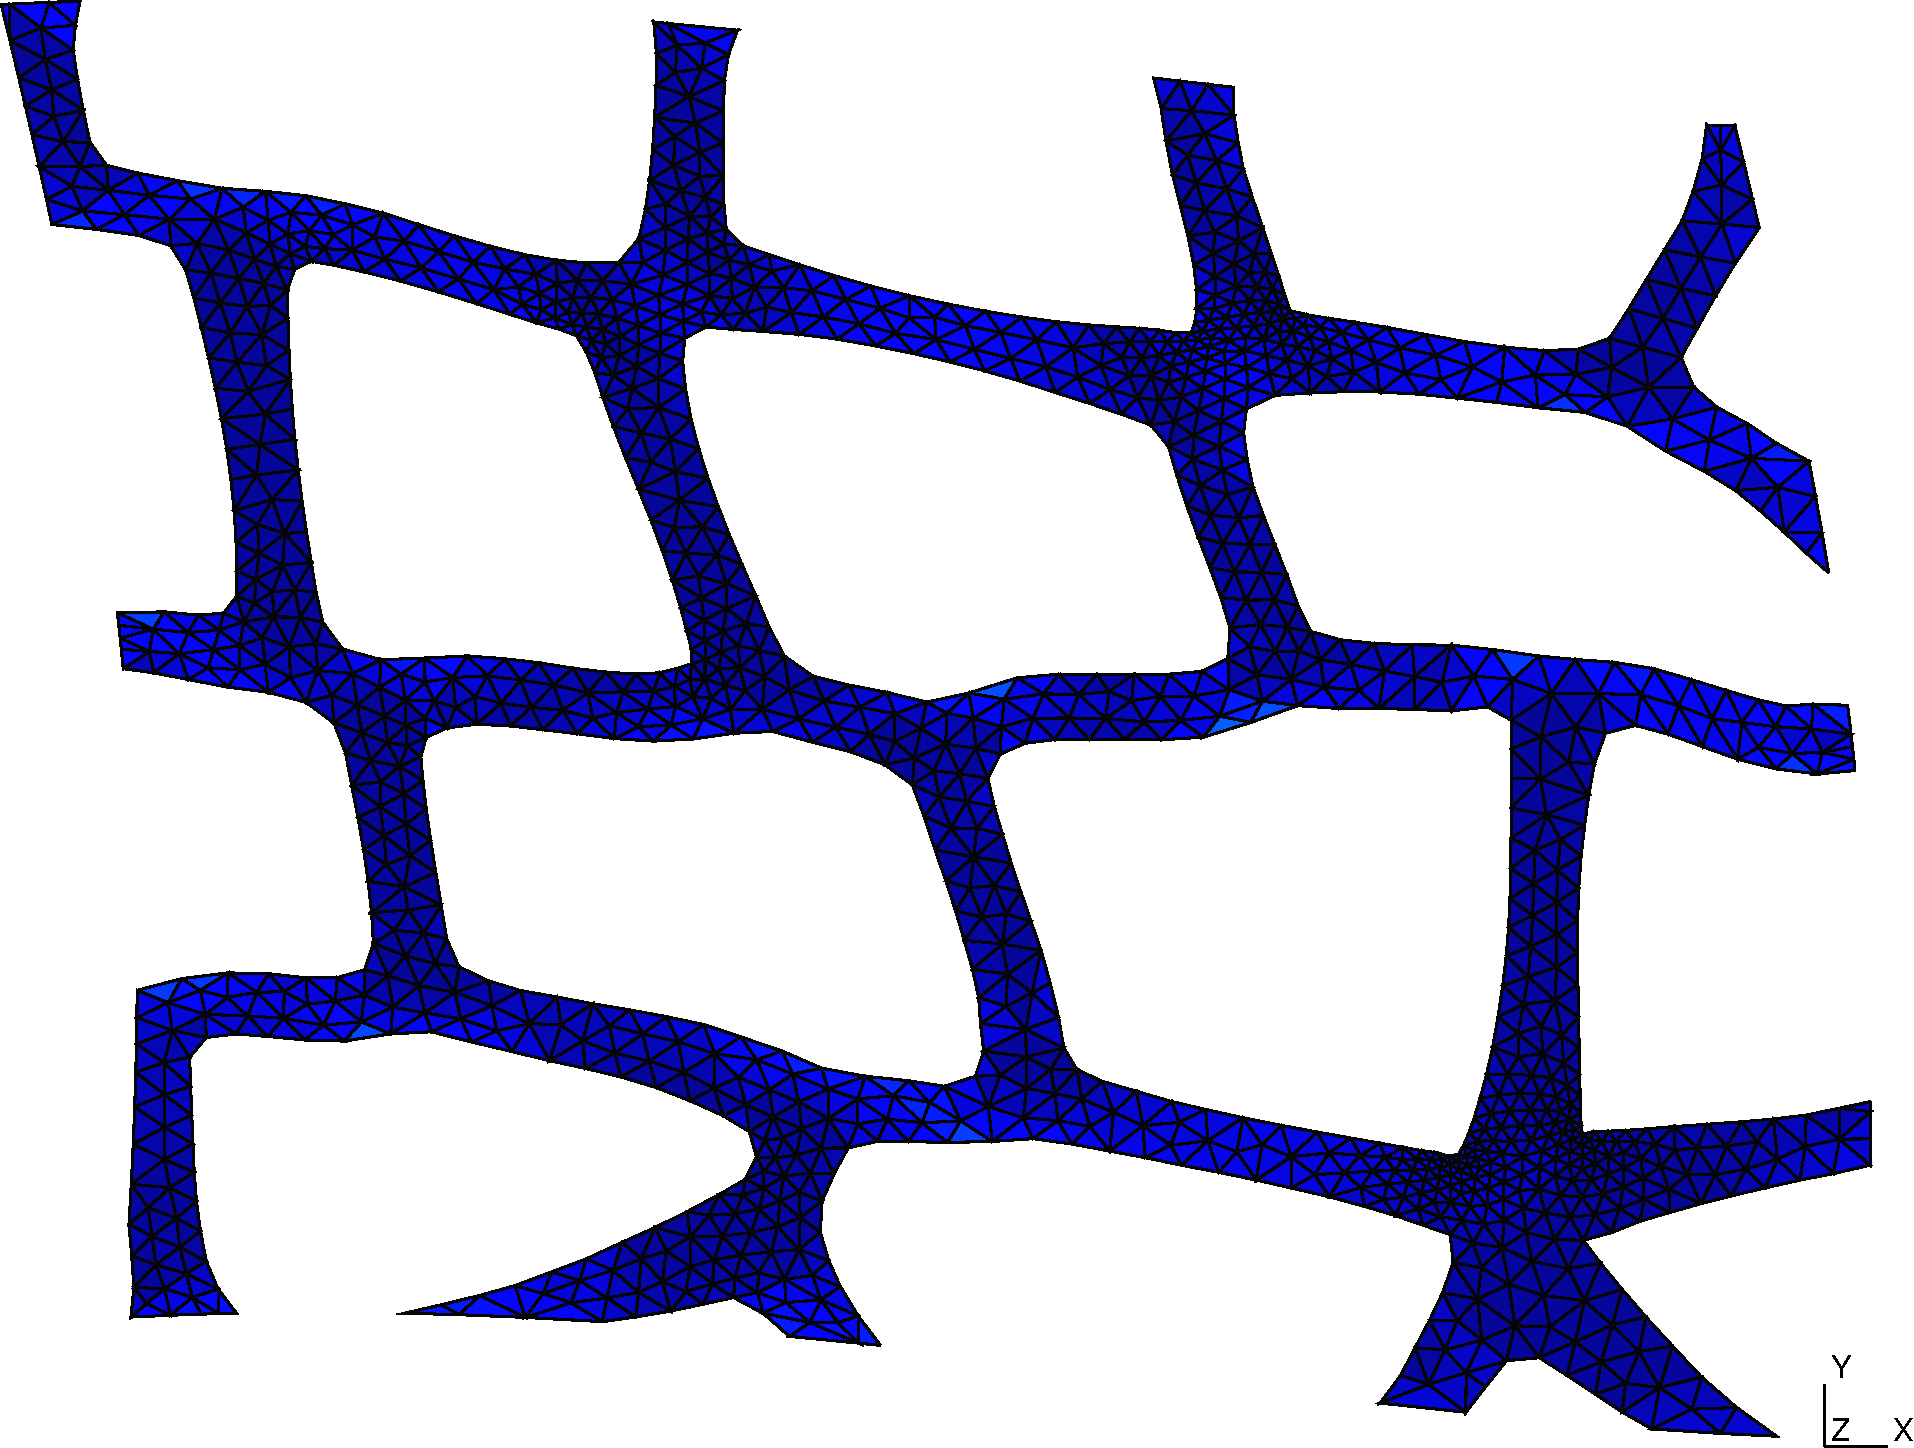
\includegraphics[height=4.cm]{eqps_23}
	\caption{}
	\end{subfigure}
	\begin{subfigure}[t]{0.45\textwidth}
		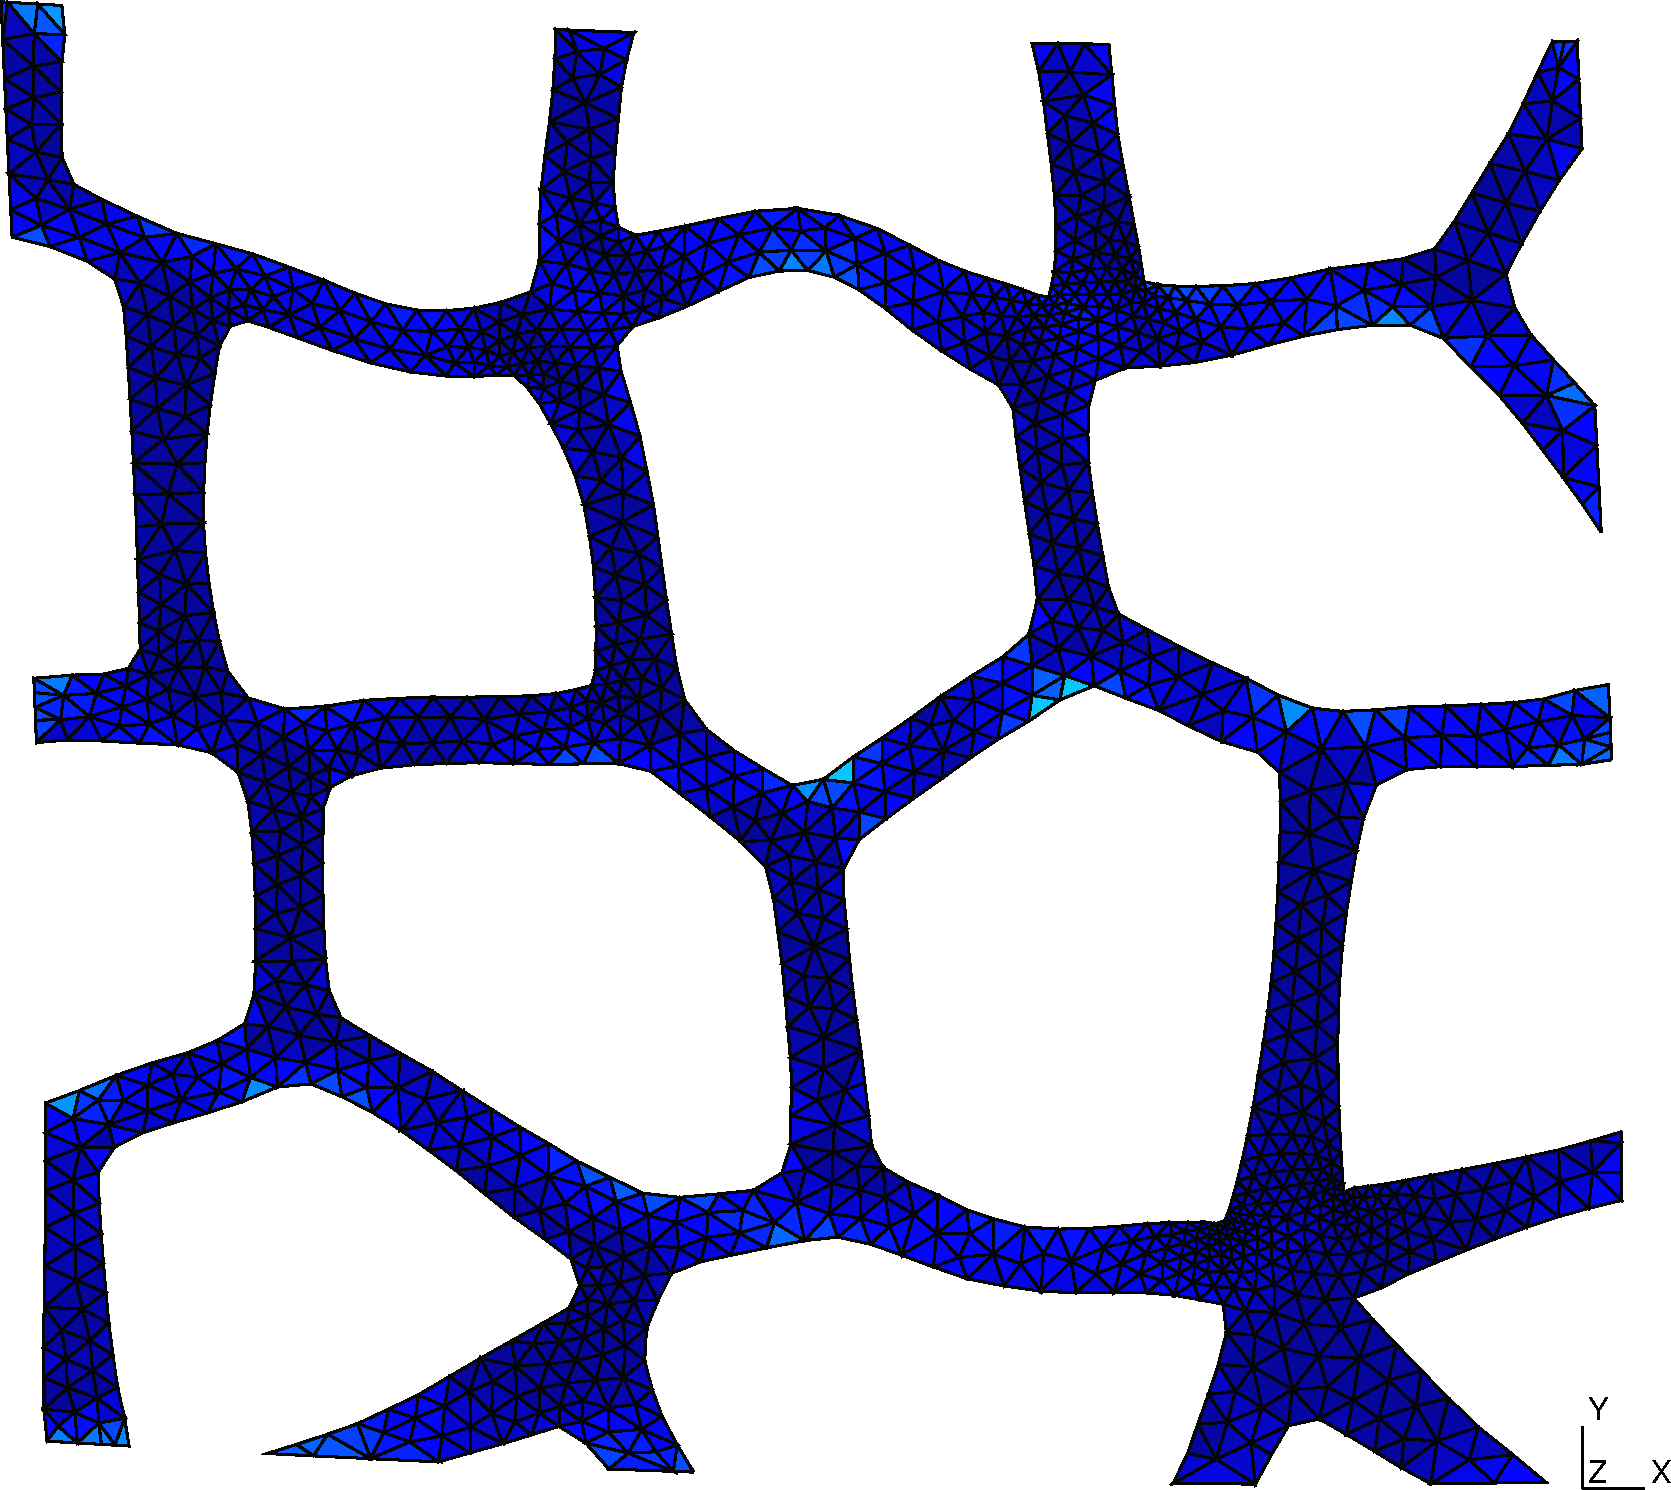
\includegraphics[height=4.cm]{eqps_42}
	\caption{}
	\end{subfigure}
	\begin{subfigure}[t]{0.45\textwidth}
		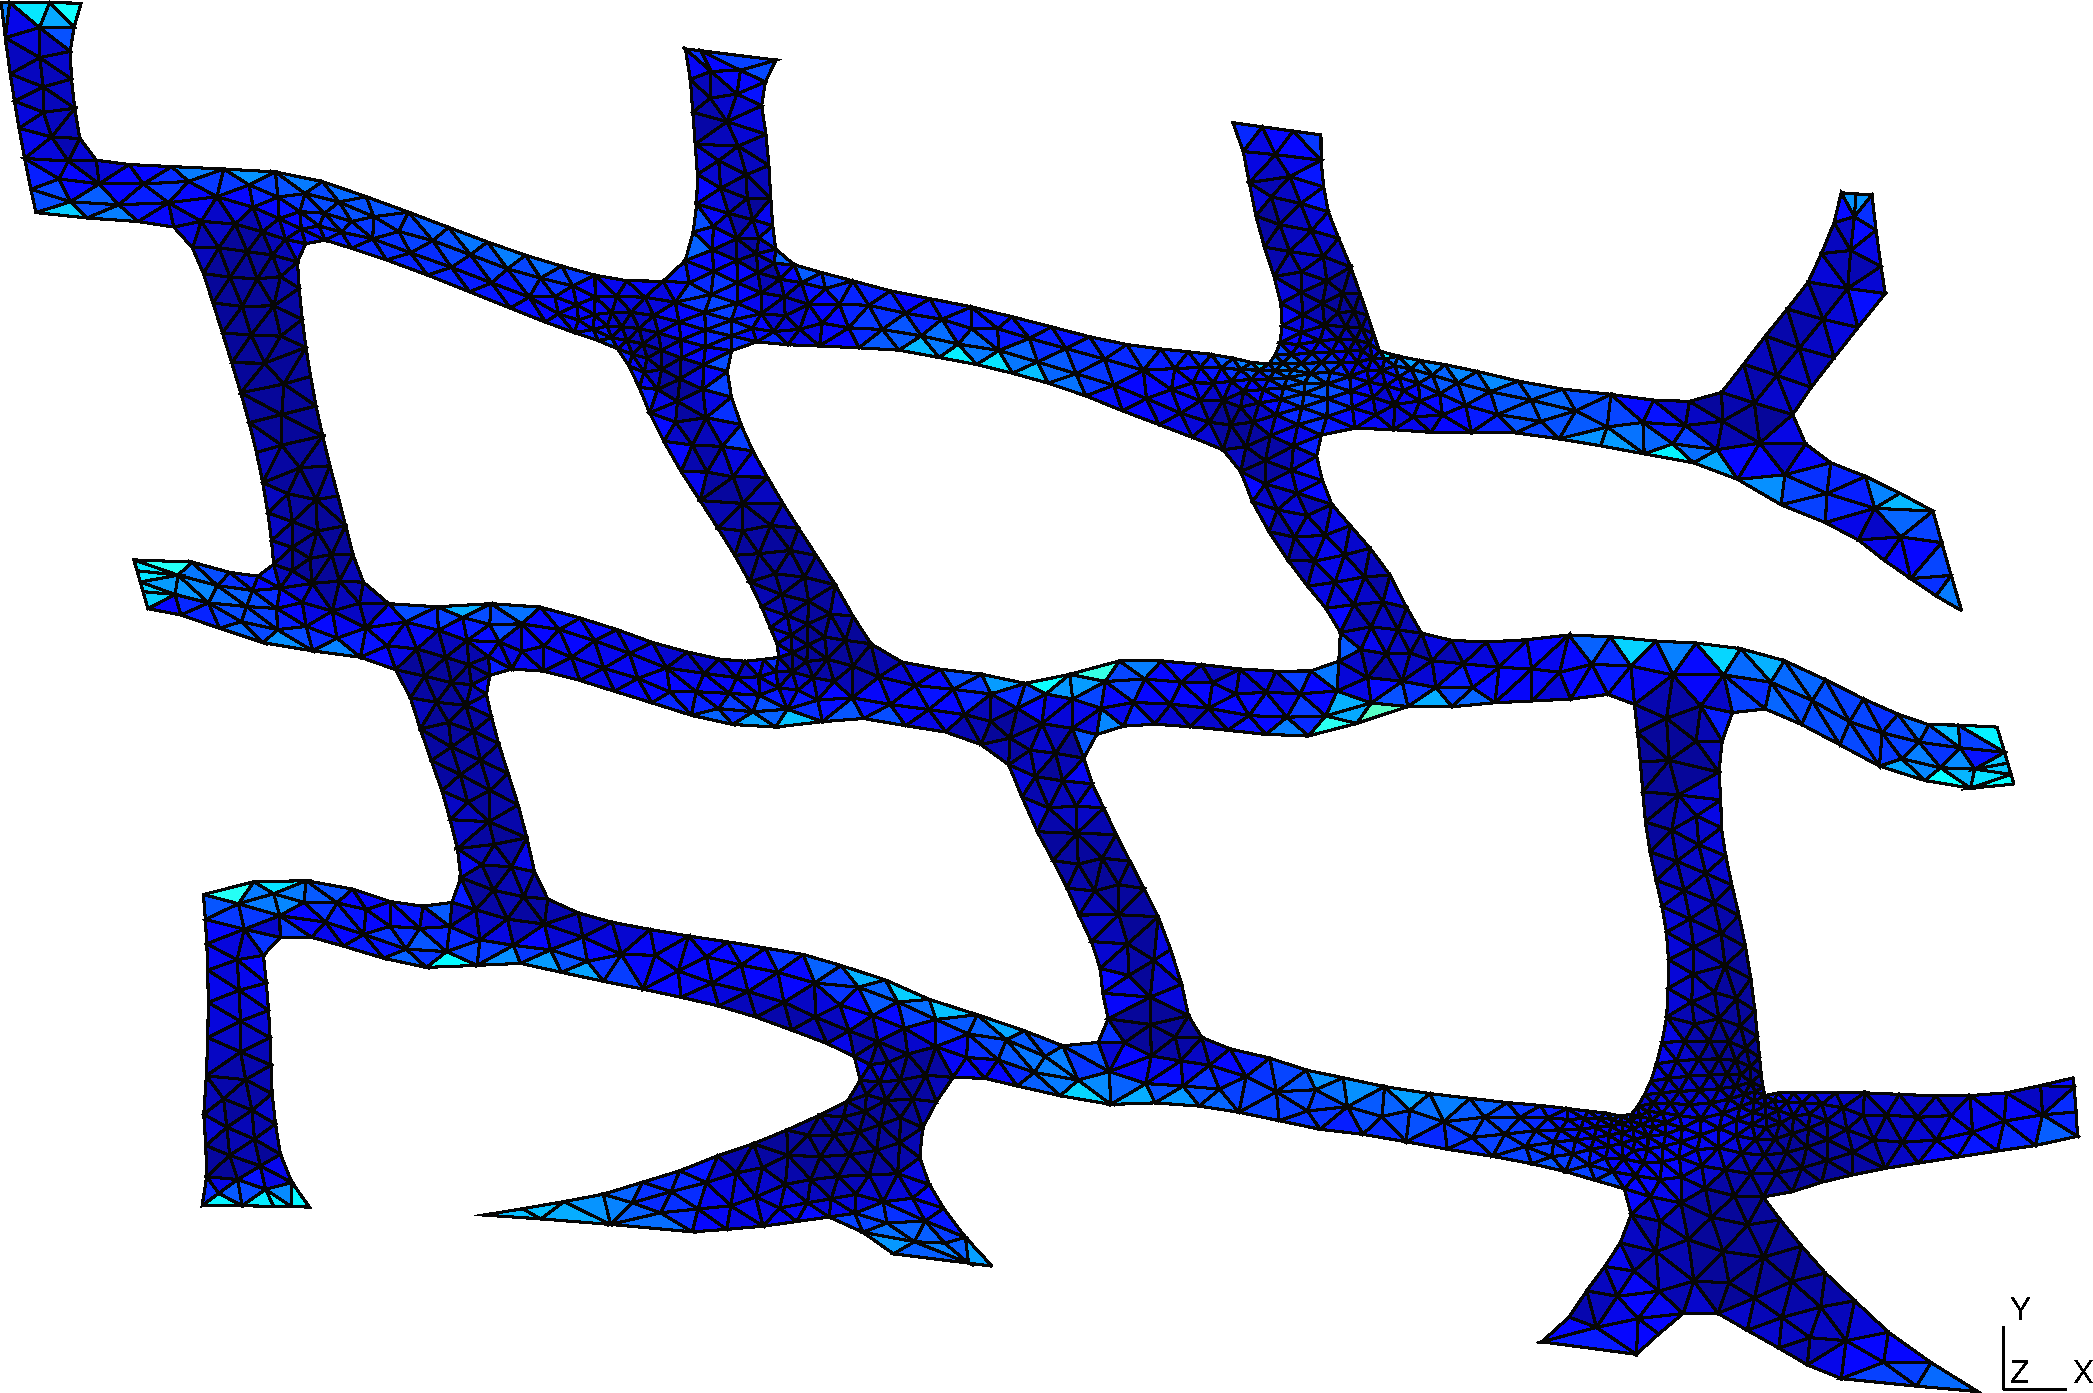
\includegraphics[height=4.cm]{eqps_73}
	\caption{}
	\end{subfigure}
	\begin{subfigure}[t]{0.45\textwidth}
		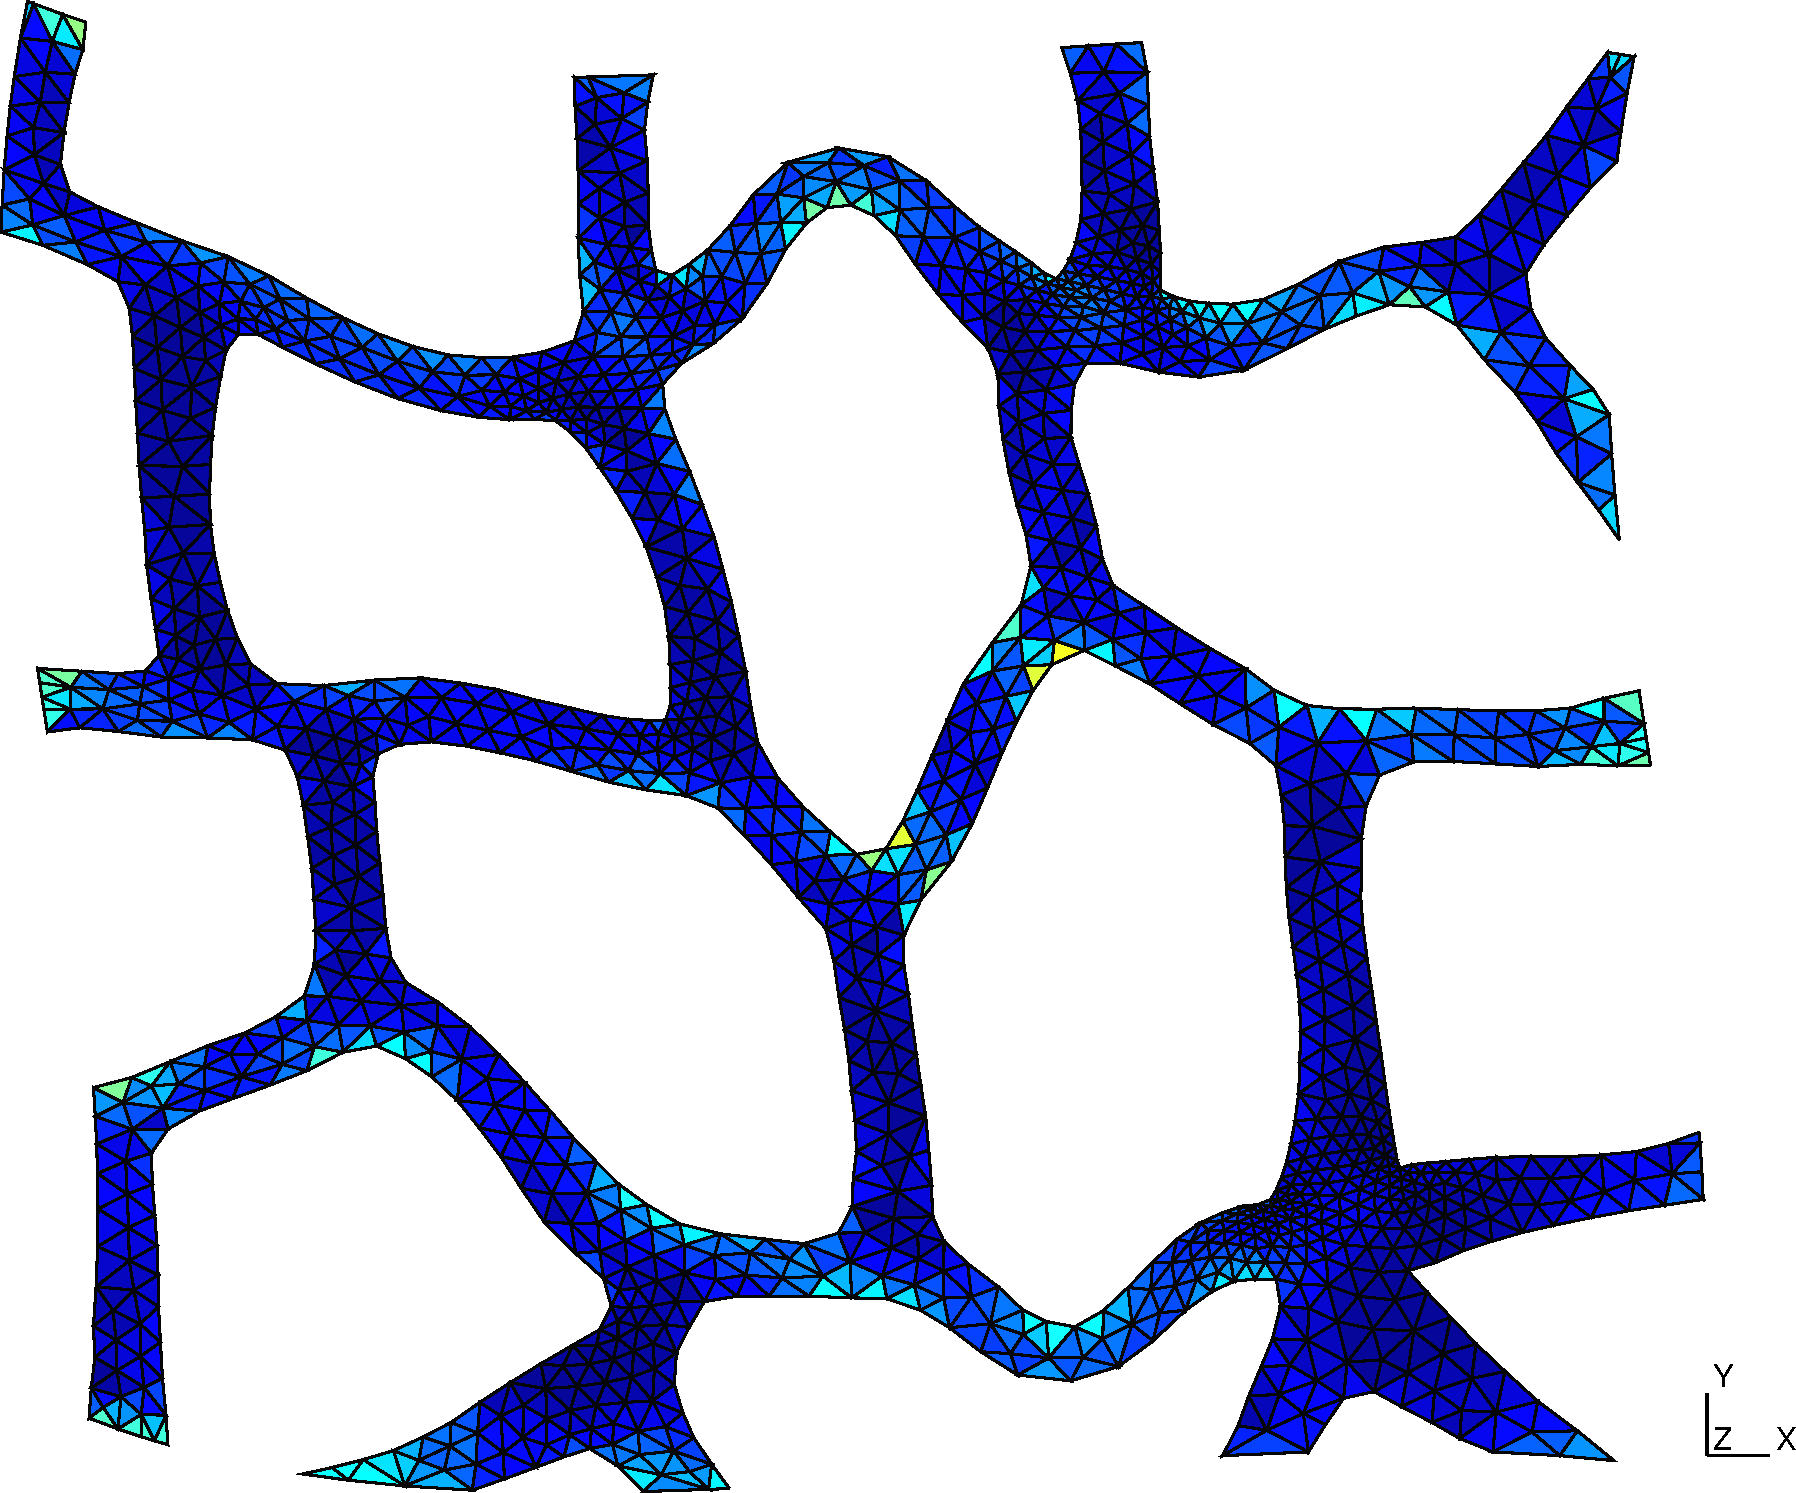
\includegraphics[height=4.cm]{eqps_99}
	\caption{}
	\end{subfigure}
	\begin{subfigure}[t]{0.45\textwidth}
		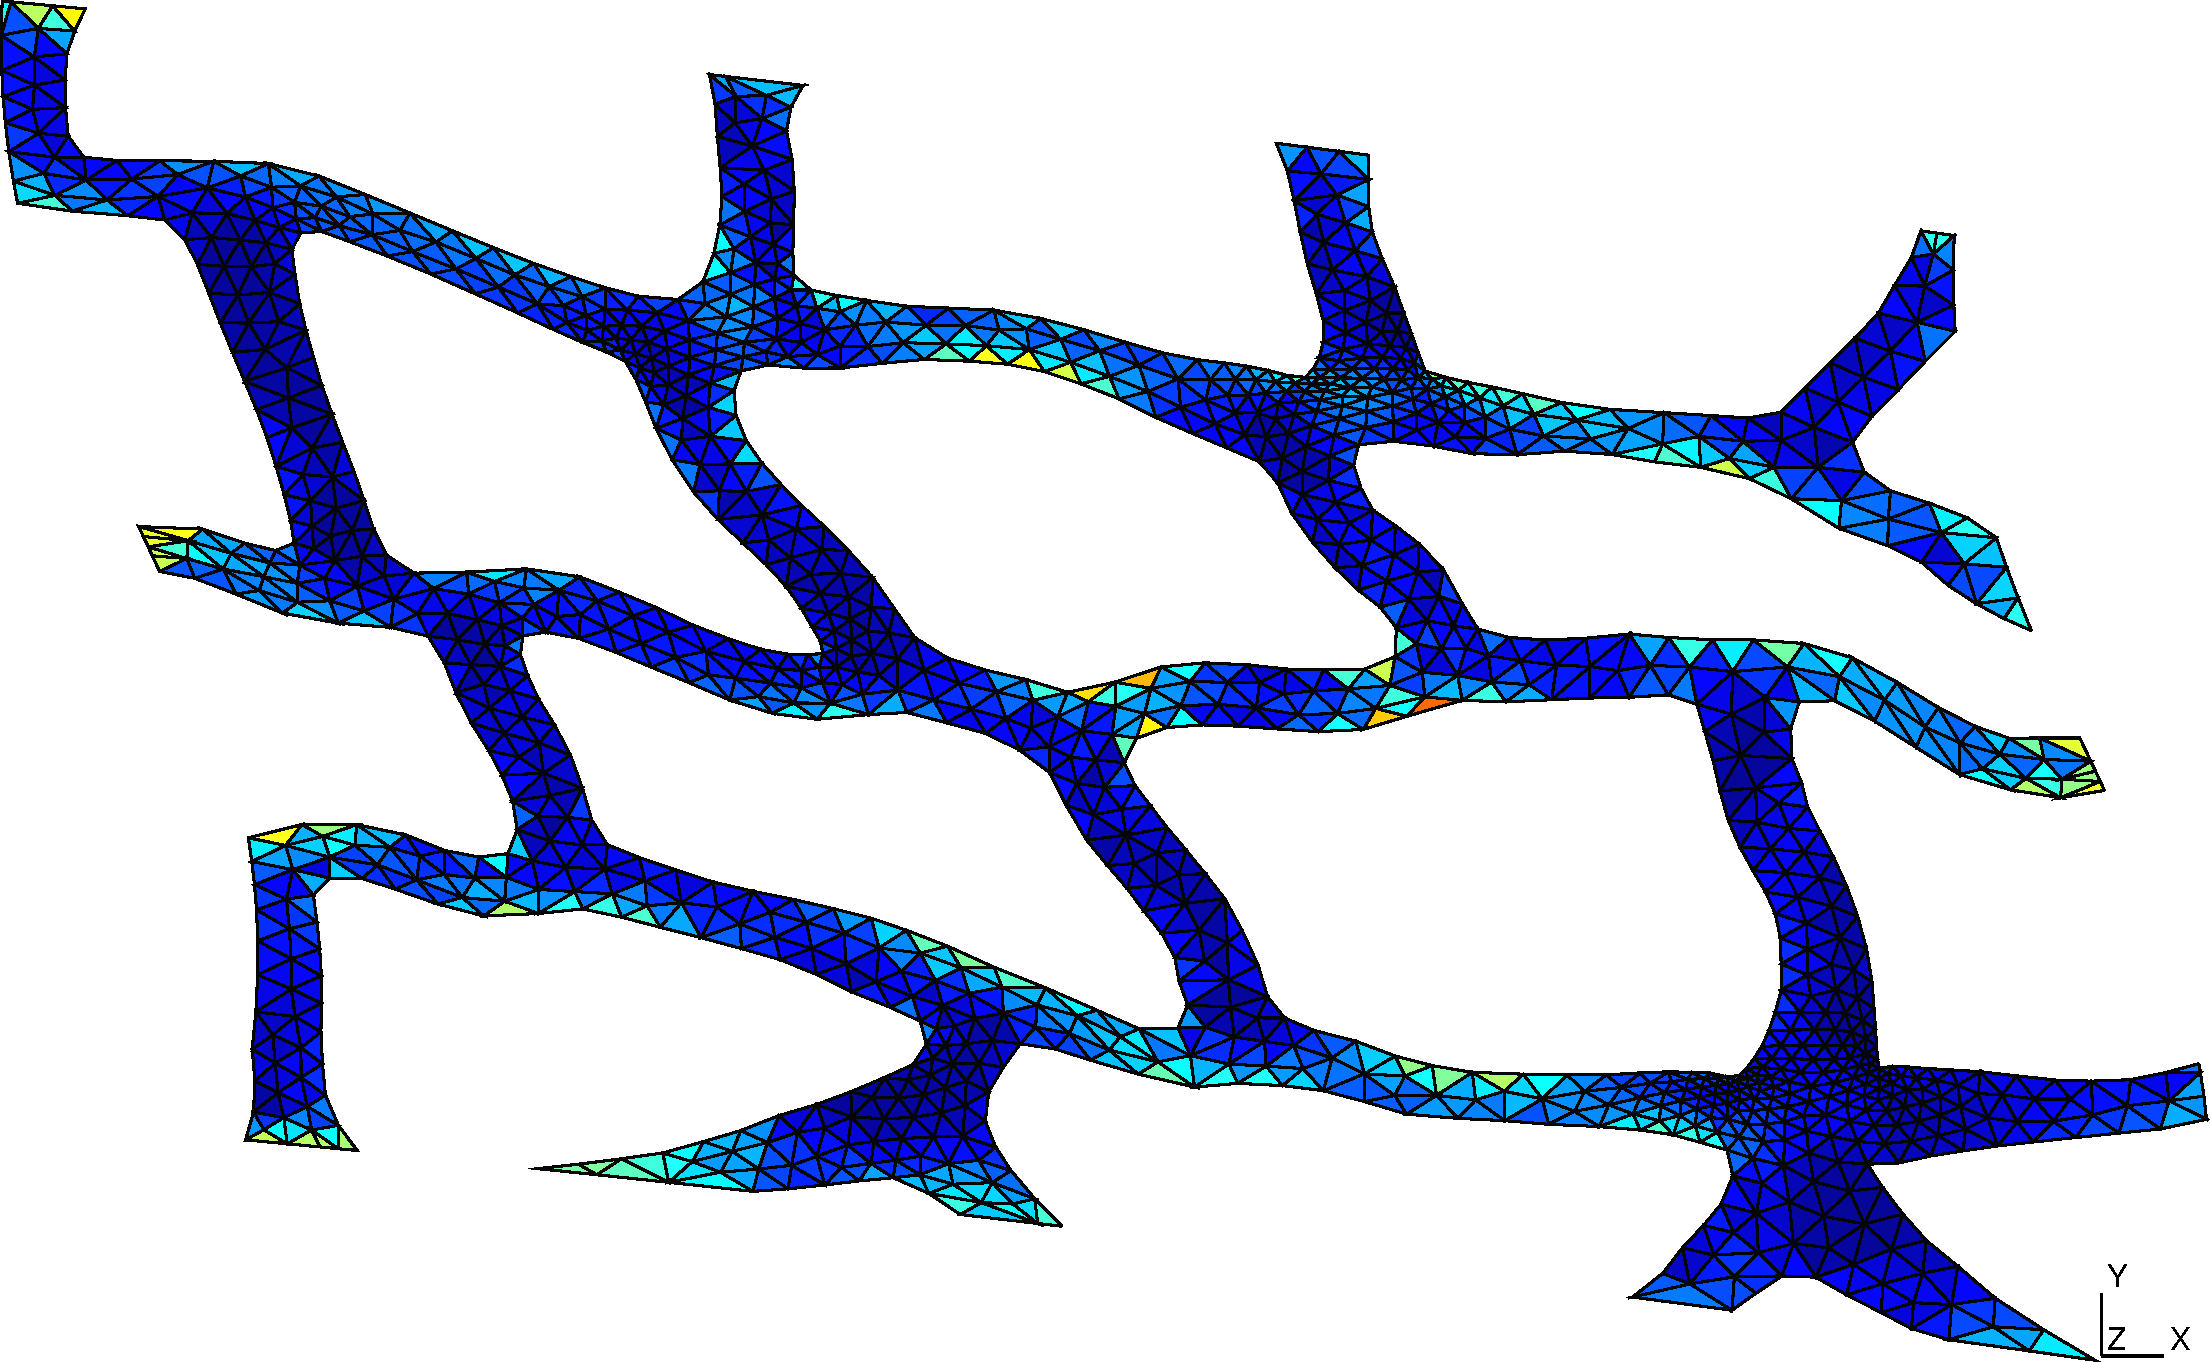
\includegraphics[height=4.cm]{eqps_136}
	\caption{}
	\end{subfigure}
	\begin{subfigure}[t]{0.5\textwidth}
		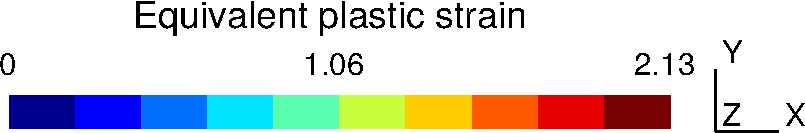
\includegraphics[width=\textwidth]{eqps_scale_cyclic}
	\end{subfigure}
	\caption{(a) - (e) Snapshots of different stages of deformation as observed for a single sample numerical analysis under repeated cyclic loading displaying the loss of unique stress-strain states that is observed under monotonic loading.}\label{fig-rnn-1-1}
\end{figure}

Figure \ref{fig-rnn-1} illustrates a set of five random path sequences. Figure \ref{fig-rnn-1-1} illustrates the behavior of the material under a simple cyclic loading. The resultant bounds of the $ 2^\text{nd} $-Piola Kirchhoff stress tensor for the training dataset is as follows:
\begin{eqnarray}\label{eq-rnn-res3}
\textbf{S}_\text{min}&=&\min\left(S_{XX}^{RNN},S_{XY}^{RNN},S_{YY}^{RNN},S_{ZZ}^{RNN}\right)\nonumber\\&=&\left[-52.04112756, -18.56087983, -39.63532748,
-14.70718438\right]\text{MPa}\nonumber
\end{eqnarray}
and
\begin{eqnarray}\label{eq-rnn-res4}
\textbf{S}_\text{max}&=&\max\left(S_{XX}^{RNN},S_{XY}^{RNN},S_{YY}^{RNN},S_{ZZ}^{RNN}\right)\nonumber\\&=&\left[24.3843425, 23.4865036, 25.9152895, 33.2079829\right]\text{MPa}.\nonumber
\end{eqnarray}

The datasets correspond to around 4000 sequences of stress responses to the random path loading with each sequence truncated at 1000 steps. Around 3000 of these have been used to train the ANN models with around 150 sequences used as validation data.

The internal state vector $ \textbf{Z} $, necessary to train the \fnn models, is comprised of the plastic part of the deformation gradient $ \{\textbf{F}^p_{XX},\textbf{F}^p_{XY},\textbf{F}^p_{YX},\textbf{F}^p_{YY},\textbf{F}^p_{ZZ}\} $ and the equivalent plastic strain $ \textbf{p} $ in 2D calculated at each Gauss-point as described in Appendix \ref{app-state}. This gives an additional $ N_{gp}\times 6$ features describing the state along with the right stretch tensor values at every step of the numerical simulation. The number of features can be brought down by the introduction of clusters as explained in Section \ref{nn-dnn-state}. To give an example, with 7 cluster based clustering, the sequences trained with RNNs correspond to around 2 million stress-strain-internal state variable each with 48 input features and 42 output features for FNN-1 and 45 input features and 4 output features for FNN-2.

\begin{figure}[]
	\centering
	\begin{subfigure}[t]{0.49\textwidth}
		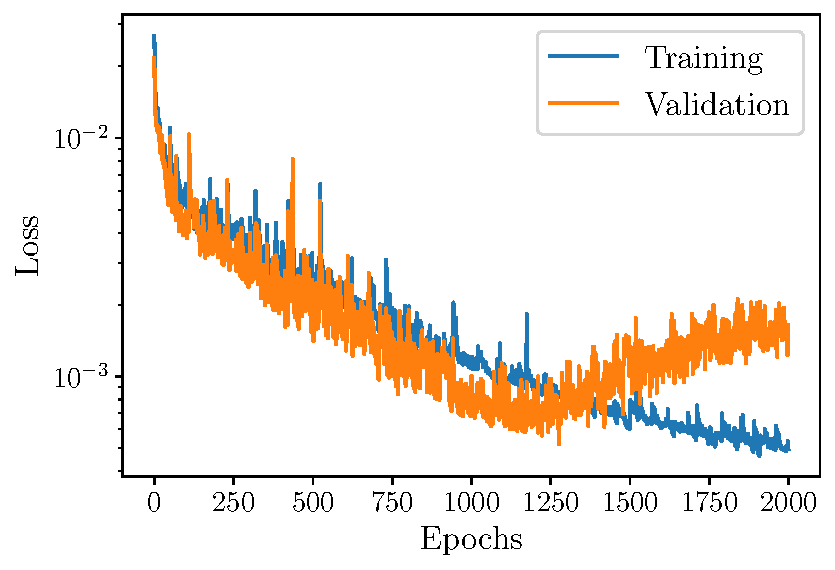
\includegraphics[width=\textwidth]{LSTM_loss_dp_02_ni1_no2}
		\caption{LSTM-RNN, Dropout 0.2}
	\end{subfigure}
	\begin{subfigure}[t]{0.49\textwidth}
		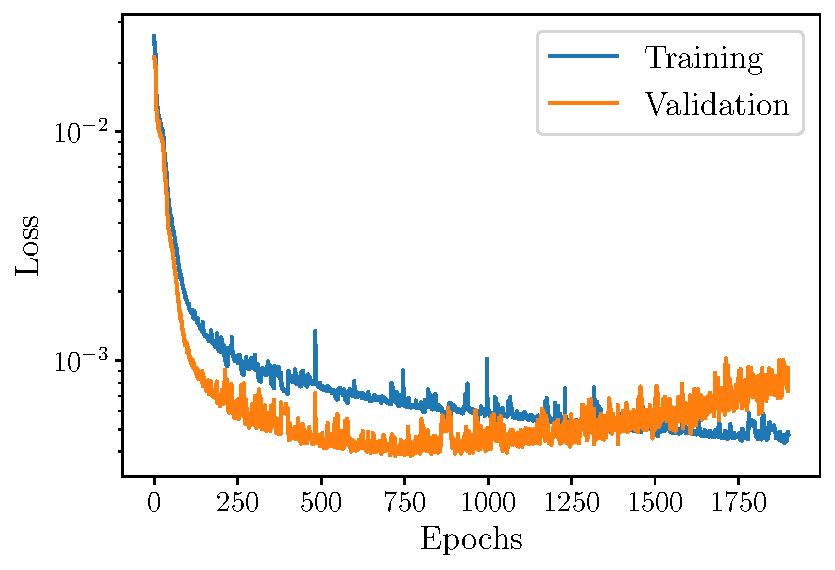
\includegraphics[width=\textwidth]{GRU_loss_dp_02_ni1_no_2}
		\caption{GRU-RNN, Dropout 0.2}
	\end{subfigure}
	\begin{subfigure}[t]{0.49\textwidth}
		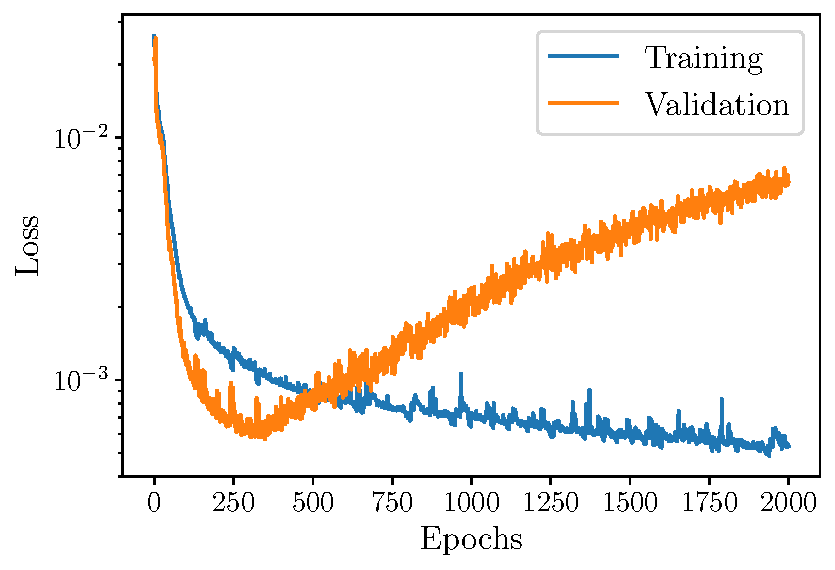
\includegraphics[width=\textwidth]{GRU_loss_dp_03_ni1_no2}
		\caption{GRU-RNN, Dropout 0.3}
	\end{subfigure}
	\begin{subfigure}[t]{0.49\textwidth}
		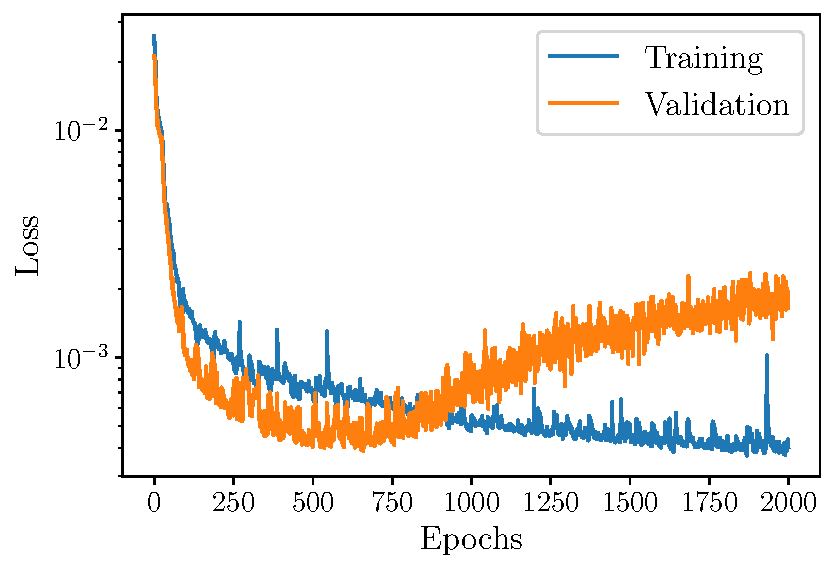
\includegraphics[width=\textwidth]{GRU_loss_dp_02_ni1_no3}
		\caption{GRU-RNN, Dropout 0.2, additional hidden layer}
	\end{subfigure}
	\caption{The training error and the validation error from the learning of (a) an LSTM based RNN model, and (b) GRU based RNN model with increasing number of training iterations (epochs) with dropout 0.2 applied following the RNN layer, with one layer of 100 nodes before and two layers of 60 nodes after the RNN layer respectively (Table \ref{tab_rnn}). (c) Effect of increasing the dropout to 0.3 as seen in the GRU based RNN module with the same architecture as (a). (d) Effect of adding another hidden layer following the RNN layer with 60 nodes while maintaining he dropout of 0.2 as seen on a GRU based RNN model.}\label{fig-nn-rnn1}
\end{figure}

\subsubsection{LSTM-RNN Model}
A summary of the LSTM based RNN model is presented in Table \ref{tab_rnn} with which the generated datasets can be trained. The input and the output layer are very similar to that of the FNN model used to predict proportional loading behavior except that the input strain and the output strain are formatted as a sequence with each individual sequence representing a single simulation (Eqs. (\ref{eq-nn-data5}) and (\ref{eq-nn-data6})). This model is very similar to the model presented in \cite{wuRecurrentNeuralNetworkaccelerated2020}. The evolution of the training error is presented in Figure \ref{fig-nn-rnn1}a.


\subsubsection{GRU-RNN Model} A GRU based RNN model (Table \ref{tab_rnn}) is very similar to that of an LSTM based RNN, with the corresponding RNN layer replaced by GRU cells. Figure \ref{fig-nn-rnn1}b presents the evolution of the training error for GRU based RNNs. 

It is very clear that the GRU-RNNs have considerably less number of parameters that need to be trained in comparison with LSTM-RNNs. Also, the learning ability of the GRU-RNNs is much faster, and this is very evident with it becoming the choice for studying plasticity dependent material behavior\cite{mozaffarDeepLearningPredicts2019,gorjiPotentialRecurrentNeural2020}.

Figure \ref{fig-nn-rnn1}c illustrates the training and the validation error on increasing the dropout in the same GRU based RNN model. It can be seen that after an initial drop in the validation error, the model overfits quite fast compared to a dropout of 0.2 possibly indicating that the network is shallow enough that increasing the dropout hinders the learning process of the model. Similarly, in Figure \ref{fig-nn-rnn1}d, one can see that the additional layer only adds more parameters inducing a quicker overfit model even though the training error is comparable to the architecture with one less layer. 

\begin{figure}[]
	\centering
	\begin{subfigure}[t]{0.49\textwidth}
		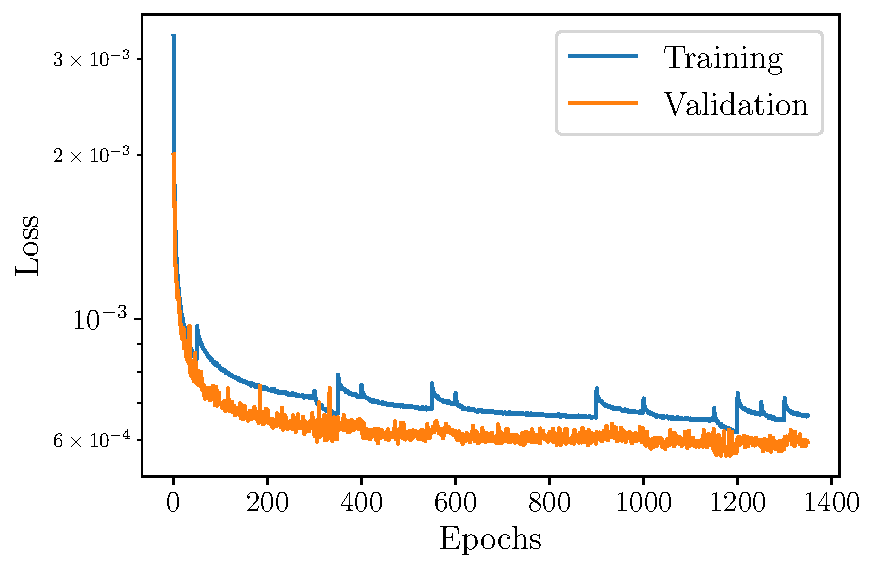
\includegraphics[width=\textwidth]{FNN1_loss}
		\caption{FNN1-\fnn for 7 clusters}
	\end{subfigure}
	\begin{subfigure}[t]{0.49\textwidth}
		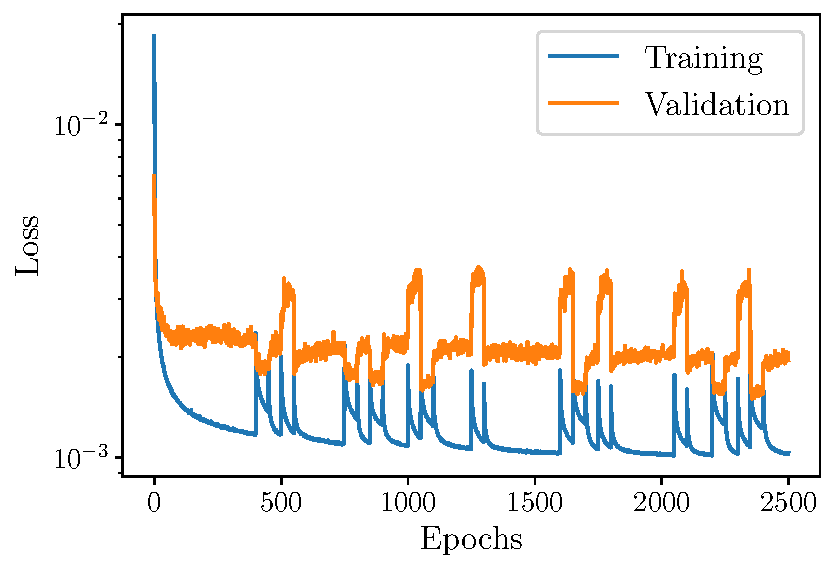
\includegraphics[width=\textwidth]{FNN2_loss}
		\caption{FNN2-\fnn for 7 clusters}
	\end{subfigure}
	%	\begin{subfigure}[t]{0.49\textwidth}
	%	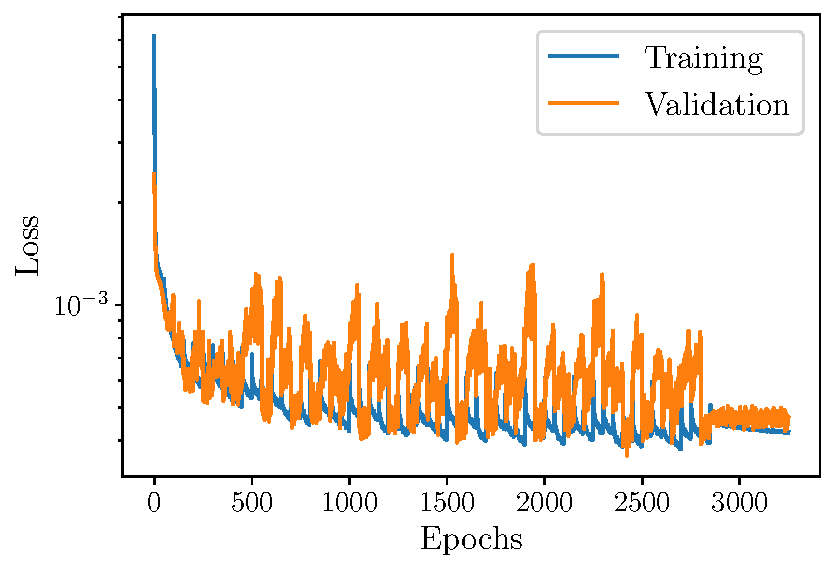
\includegraphics[width=\textwidth]{FNN2-FNN-1-15_training_validation_loss}
	%	\caption{}
	%\end{subfigure}
	%	\begin{subfigure}[t]{0.49\textwidth}
	%	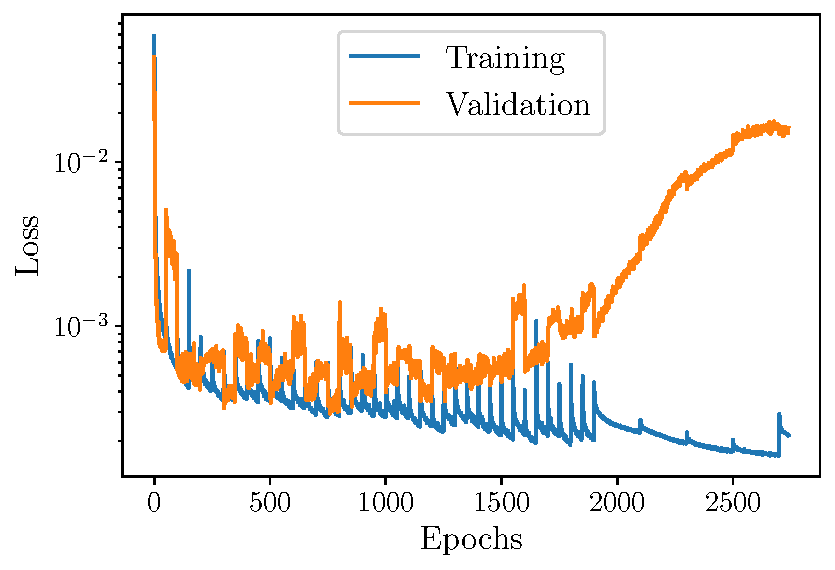
\includegraphics[width=\textwidth]{FNN2-FNN-2-15_training_validation_loss}
	%	\caption{}
	%\end{subfigure}
	\begin{subfigure}[t]{0.49\textwidth}
		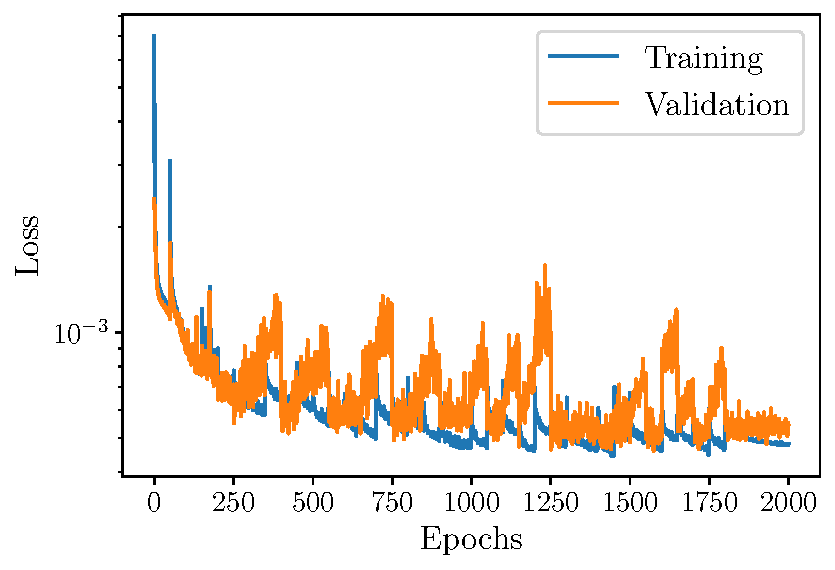
\includegraphics[width=\textwidth]{FNN2-FNN-1-30_training_validation_loss}
		\caption{FNN1-\fnn for 30 clusters}
	\end{subfigure}
	\begin{subfigure}[t]{0.49\textwidth}
		\includegraphics[width=\textwidth]{FNN2-FNN-2-30_training_validation_loss}
		\caption{FNN2-\fnn for 30 clusters}
	\end{subfigure}
	\caption{The training error and the validation error from the learning of the two \fnn models corresponding to the number of clusters used with increasing number of training iterations (epochs).}\label{fig-nn-rnn2}
\end{figure}

\subsubsection{\fnn Model} As explained in Section \ref{nn-dnn}, an \fnn model is simply an extension of the FNN model that has been implemented twice. Tables \ref{tab_fnn2-fnn1} and \ref{tab_fnn2-fnn2} summarizes the FNN1-\fnn models and FNN2-\fnn models respectively and present a comparison on the number of parameters necessary depending on the number of state variables chosen to represent the state of the material. It is very evident that the number of trainable parameters drastically increases with an increase in the number of features, and this justifies the implementation of clustering of the features to have a control on the network. With so many parameters involved, there is a real chance of model overfitting, where the model ``learns'' from the data rather than ``generalizing'' which can be visualized during training using the validation datasets.


Figure \ref{fig-nn-rnn2} presents the evolution of training error for the two \fnn models while training with differing number of features by controlling the number of clusters used. It can be seen that the models can generalize the behavior with low number of features, and thus it is not necessary to resort to higher number of features to represent the behavior of the materials.

\begin{sidewaystable}
	\centering
	\caption{Sample RNN models with the input layer, four hidden layers of which one is RNN based and the output layers outlined, along with the number of parameters in each layer and the parameters to be trained. `X' denotes variable length of the input sequence assuming one training sequence. The LSTM cell outputs a cell state which the GRU cell does not.}\label{tab_rnn}
	\centering
	\begin{tabular}{|>{\raggedright\arraybackslash}m{0.2\textwidth}|>{\raggedright}m{0.2\textwidth}|m{0.16\textwidth}|>{\raggedright}m{0.2\textwidth}|m{0.16\textwidth}|}
		\hline
		\rule{0pt}{4ex}    
		\textbf{Layer (type)} & \textbf{LSTM based RNN \reda{Weights shape}/ \blue{Bias shape}/ Output Shape} & \textbf{Number of Parameters}& \textbf{GRU based RNN \reda{Weights shape}/ \blue{Bias shape}/ Output Shape} & \textbf{Number of Parameters}\\
		\hline 
		\rule{0pt}{4ex}    
		Input (InputLayer) & (X, 3) & 0 & (X, 3) & 0 \\
		\hline 
		\rule{0pt}{4ex}    
		FNN-Layer1 (Dense) & \reda{(3, 100)}, \blue{(100)}, (X, 100) & 400 & \reda{(X, 3, 100)}, \blue{(X, 100)}, (X, 100) & 400 \\
		\hline 
		\rule{0pt}{4ex}    
		RNN-Layer & \reda{(100, 240)}, \reda{(60, 240)}, \blue{(240)}, (X, 60), (60), (60) & 38640 & \reda{(100, 180)}, \reda{(60, 180)}, \blue{(2, 180)}, (X, 60), (60) & 29160 \\
		\hline 
		\rule{0pt}{4ex}    
		Dropout (Dropout) & (X, 60) & 0 & (X, 60) & 0 \\
		\hline 
		\rule{0pt}{4ex}    
		FNN-Layer2 (Dense) & \reda{(60, 60)}, \blue{(60)}, (X, 60) & 3660 & \reda{(60, 60)}, \blue{(60)}, (X,60) & 3660 \\
		\hline 
		\rule{0pt}{4ex}    
		FNN-Layer3 (Dense) & \reda{(60, 60)}, \blue{(60)}, (X, 60) & 3660 & \reda{(60, 60)}, \blue{(60)}, (X, 60) & 3660 \\
		\hline 
		\rule{0pt}{4ex}    
		Output (Dense) & \reda{(60, 4)}, \blue{(4)}, (X, 4) & 244 &\reda{(60, 4)}, \blue{(4)}, (X, 4) & 244 \\
		\hline 
		
		Total parameters & \multicolumn{2}{l|}{
			\rule{0pt}{4ex}    
			46604} & \multicolumn{2}{l|}{
			\rule{0pt}{4ex}    
			37124}\\
		\hline 
		Trainable parameters & \multicolumn{2}{l|}{
			\rule{0pt}{4ex}    
			46604} & \multicolumn{2}{l|}{
			\rule{0pt}{4ex}    
			37124}\\
		\hline 
		Non-trainable parameters  & \multicolumn{2}{l|}{
			\rule{0pt}{4ex}    
			0} & \multicolumn{2}{l|}{
			\rule{0pt}{4ex}    
			0}\\
		\hline 
	\end{tabular}	
\end{sidewaystable}


\subsubsection{RNN Predictions} To test the predictability of the RNN based models, a new sequence of random path strain, which was not used in the training and validation of the RNN model, can feed the model and the stress predictions can then be compared to the simulation results. Figure \ref{fig-nn-rnn3} illustrates some results where a comparison between the LSTM based and GRU based RNN models are tested for their prediction capabilities. 

\begin{figure}
	\centering
	\begin{subfigure}[t]{0.45\textwidth}
		\includegraphics[width=\textwidth]{RNN_GRU_LSTM_200_random0}
	\end{subfigure}
	\begin{subfigure}[t]{0.45\textwidth}
		\includegraphics[width=\textwidth]{RNN_GRU_LSTM_200_random1}
	\end{subfigure}
	\begin{subfigure}[t]{0.45\textwidth}
		\includegraphics[width=\textwidth]{RNN_GRU_LSTM_200_random3}
	\end{subfigure}
	\begin{subfigure}[t]{0.45\textwidth}
		\includegraphics[width=\textwidth]{RNN_GRU_LSTM_200_random4}
	\end{subfigure}
	\caption{Comparison between the LSTM and GRU based RNN predictions and the DNS results (in blue) of the stress (in MPa) for randomly selected strain path shown here for 200 steps for clarity.}\label{fig-nn-rnn3}
\end{figure}

The two models show very similar results with the GRU model being slightly better with its predictions. GRU models, which have comparatively lower number of parameters to be trained, and which also generalizes the data faster as compared to LSTM models, are definitely a preferable choice for RNN models.

\begin{sidewaystable}
	\centering
	\caption{Sample FNN1-\fnn models with the input layer, three hidden layers and the output layers outlined, along with the number of parameters in each layer and the parameters to be trained. For comparison, differing number of clusters used for representing the internal state variable along with the gauss-point based representation for $ N_{gp}=2000 $ is presented. `X' denotes variable input size at any given training iteration.}\label{tab_fnn2-fnn1}
	\begin{tabular}{|>{\raggedright\arraybackslash}m{0.12\textwidth}|>{\raggedright}m{0.15\textwidth}|m{0.10\textwidth}|>{\raggedright}m{0.15\textwidth}|m{0.10\textwidth}|>{\raggedright}m{0.15\textwidth}|m{0.10\textwidth}|}
		\hline 
		\rule{0pt}{4ex}    
		\textbf{Layer (type)} & \textbf{7 Clusters} \reda{Weights shape}/ \textbf{\blue{Bias shape}}/ \textit{Output Shape} & \textbf{Number of Parameters}& \textbf{15 Clusters} \reda{Weights shape}/ \textbf{\blue{Bias shape}}/ \textit{Output Shape} & \textbf{Number of Parameters}& \textbf{$ N_{gp}=2000 $} \reda{Weights shape}/ \textbf{\blue{Bias shape}}/ \textit{Output Shape} & \textbf{Number of Parameters}\\
		\hline 
		\rule{0pt}{4ex}    
		Input (InputLayer) & \textit{(X, 48)} & 0 & \textit{(X, 96)} & 0 & \textit{(X, 12006)} & 0\\
		\hline 
		\rule{0pt}{4ex}    
		FNN-Layer1 (Dense) & \reda{(48, 200)}, \textbf{\blue{(200)}}, \textit{(X, 200)} & 9800 & \reda{(96, 200)}, \textbf{\blue{(200)}}, \textit{(X, 200)} & 19400 & \reda{(12006, 200)}, \textbf{\blue{(200)}}, \textit{(X, 200)} & 2401400\\
		\hline 
		\rule{0pt}{4ex}    
		Dropout (Dropout) & \textit{(X, 200)} & 0 & \textit{(X, 200)} & 0 & \textit{(X, 200)} & 0\\
		\hline 
		\rule{0pt}{4ex}    
		FNN-Layer2 (Dense) & \reda{(200, 100)}, \textbf{\blue{(100)}}, \textit{(X, 100)} & 20100 & \reda{(200, 100)}, \textbf{\blue{(100)}}, \textit{(X, 100)} & 20100 & \reda{(200, 100)}, \textbf{\blue{(100)}}, \textit{(X, 100)} & 20100\\
		\hline 
		\rule{0pt}{4ex}    
		FNN-Layer3 (Dense) & \reda{(100, 100)}, \textbf{\blue{(100)}}, \textit{(X, 100)} & 10100 & \reda{(100, 100)}, \textbf{\blue{(100)}}, \textit{(X, 100)} & 10100 & \reda{(100, 100)}, \textbf{\blue{(100)}}, \textit{(X, 100)} & 10100\\
		\hline 
		\rule{0pt}{4ex}    
		Output (Dense) & \reda{(100, 42)}, \textbf{\blue{(42)}}, \textit{(X, 42)} & 4242 & \reda{(100, 90)}, \textbf{\blue{(90)}}, \textit{(X, 90)} & 9090 & \reda{(100, 12000)}, \textbf{\blue{(12000)}}, \textit{(X, 12000)} & 1212000\\
		\hline 
		
		Total parameters & \multicolumn{2}{l|}{
			\rule{0pt}{4ex}    
			44242} & \multicolumn{2}{l|}{
			\rule{0pt}{4ex}    
			58690} & \multicolumn{2}{l|}{
			\rule{0pt}{4ex}    
			3643600}\\
		\hline 
		Trainable parameters & \multicolumn{2}{l|}{
			\rule{0pt}{4ex}    
			44242} & \multicolumn{2}{l|}{
			\rule{0pt}{4ex}    
			58690} & \multicolumn{2}{l|}{
			\rule{0pt}{4ex}    
			3643600}\\
		\hline 
		Non-trainable parameters  & \multicolumn{2}{l|}{
			\rule{0pt}{4ex}    
			0} & \multicolumn{2}{l|}{
			\rule{0pt}{4ex}    
			0} & \multicolumn{2}{l|}{
			\rule{0pt}{4ex}    
			0}\\
		\hline 
	\end{tabular}	
\end{sidewaystable}
\begin{sidewaystable}
	\centering
	\caption{Sample FNN2-\fnn models with the input layer, three hidden layers and the output layers outlined, along with the number of parameters in each layer and the parameters to be trained. For comparison, differing number of clusters used for representing the internal state variable along with the gauss-point based representation for $ N_{gp}=2000 $ is presented. `X' denotes variable input size at any given training iteration.}\label{tab_fnn2-fnn2}
	\begin{tabular}{|>{\raggedright\arraybackslash}m{0.12\textwidth}|>{\raggedright}m{0.15\textwidth}|m{0.10\textwidth}|>{\raggedright}m{0.15\textwidth}|m{0.10\textwidth}|>{\raggedright}m{0.15\textwidth}|m{0.10\textwidth}|}
		\hline 
		\rule{0pt}{4ex}    
		\textbf{Layer (type)} & \textbf{7 Clusters} \reda{Weights shape}/ \textbf{\blue{Bias shape}}/ \textit{Output Shape} & \textbf{Number of Parameters}& \textbf{15 Clusters} \reda{Weights shape}/ \textbf{\blue{Bias shape}}/ \textit{Output Shape} & \textbf{Number of Parameters}& \textbf{$ N_{gp}=2000 $} \reda{Weights shape}/ \textbf{\blue{Bias shape}}/ \textit{Output Shape} & \textbf{Number of Parameters}\\
		\hline 
		\rule{0pt}{4ex}    
		Input (InputLayer) & \textit{(X, 45)} & 0 & \textit{(X, 93)} & 0 & \textit{(X, 12003)} & 0\\
		\hline 
		\rule{0pt}{4ex}    
		FNN-Layer1 (Dense) & \reda{(45, 200)}, \textbf{\blue{(200)}}, \textit{(X, 200)} & 9200 & \reda{(93, 200)}, \textbf{\blue{(200)}}, \textit{(X, 200)} & 18800 & \reda{(12003, 200)}, \textbf{\blue{(200)}}, \textit{(X, 200)} & 2400800\\
		\hline 
		\rule{0pt}{4ex}    
		Dropout (Dropout) & \textit{(X, 200)} & 0 & \textit{(X, 200)} & 0 & \textit{(X, 200)} & 0\\
		\hline 
		\rule{0pt}{4ex}    
		FNN-Layer2 (Dense) & \reda{(200, 100)}, \textbf{\blue{(100)}}, \textit{(X, 100)} & 20100 & \reda{(200, 100)}, \textbf{\blue{(100)}}, \textit{(X, 100)} & 20100 & \reda{(200, 100)}, \textbf{\blue{(100)}}, \textit{(X, 100)} & 20100\\
		\hline 
		\rule{0pt}{4ex}    
		FNN-Layer3 (Dense) & \reda{(100, 100)}, \textbf{\blue{(100)}}, \textit{(X, 100)} & 10100 & \reda{(100, 100)}, \textbf{\blue{(100)}}, \textit{(X, 100)} & 10100 & \reda{(100, 100)}, \textbf{\blue{(100)}}, \textit{(X, 100)} & 10100\\
		\hline 
		\rule{0pt}{4ex}    
		Output (Dense) & \reda{(100, 4)}, \textbf{\blue{(4)}}, \textit{(X, 4)} & 404 & \reda{(100, 4)}, \textbf{\blue{(4)}}, \textit{(X, 4)} & 404 & \reda{(100, 4)}, \textbf{\blue{(4)}}, \textit{(X, 4)} & 404\\
		\hline 
		
		Total parameters & \multicolumn{2}{l|}{
			\rule{0pt}{4ex}    
			39804} & \multicolumn{2}{l|}{
			\rule{0pt}{4ex}    
			49404} & \multicolumn{2}{l|}{
			\rule{0pt}{4ex}    
			2431404}\\
		\hline 
		Trainable parameters & \multicolumn{2}{l|}{
			\rule{0pt}{4ex}    
			39804} & \multicolumn{2}{l|}{
			\rule{0pt}{4ex}    
			49404} & \multicolumn{2}{l|}{
			\rule{0pt}{4ex}    
			2431404}\\
		\hline 
		Non-trainable parameters  & \multicolumn{2}{l|}{
			\rule{0pt}{4ex}    
			0} & \multicolumn{2}{l|}{
			\rule{0pt}{4ex}    
			0} & \multicolumn{2}{l|}{
			\rule{0pt}{4ex}    
			0}\\
		\hline 
	\end{tabular}	
\end{sidewaystable}

\subsubsection{\fnn Predictions} \fnn models can be trained based on random state combinations, and to test its predictability, a sequence of the state combination from an individual simulation can be used. Figure \ref{fig-nn-rnn4} presents the predictions for one such simulation sequence. In this test, a one step prediction is assumed, where the model predicts only one future step and not the entire sequence of stress-states on the go. The internal state variables, initialized as zero, are sequentially predicted by the trained FNN-1 of the \fnn model which is then used as an input for the trained FNN-2 of the \fnn model along with the loading to obtain the stress predictions. The results are presented for different number of clusters that have been used to represent the state of the material. It is very clear that the lower number of clusters results in lesser number of parameters that need to be trained, and thus a better model that can generalize the data. 

Figure \ref{fig-nn-rnn4-1} illustrates the issue of attempting sequence prediction in comparison with one step prediction. Sequence prediction makes use of only the initial state variables and the sequence of loading in an attempt to predict the entire behavior of the material. However, it fails in doing so as the error accumulation triggers a chain of false results ending with nonsense values.

\begin{figure}
	\centering
	\begin{subfigure}[t]{0.45\textwidth}
		\includegraphics[width=\textwidth]{FNN2_predict_random_short_0}
	\end{subfigure}
	\begin{subfigure}[t]{0.45\textwidth}
		\includegraphics[width=\textwidth]{FNN2_predict_random_short_1}
	\end{subfigure}
	\begin{subfigure}[t]{0.45\textwidth}
		\includegraphics[width=\textwidth]{FNN2_predict_random_short_3}
	\end{subfigure}
	\begin{subfigure}[t]{0.45\textwidth}
		\includegraphics[width=\textwidth]{FNN2_predict_random_short_4}
	\end{subfigure}
	\caption{Comparison between different clusters (C) based \fnn predictions and the DNS results (in blue) of the stress (in MPa) for randomly selected strain path shown here for 200 steps for clarity.}\label{fig-nn-rnn4}
\end{figure}

\begin{figure}
	\centering
	\begin{subfigure}[t]{0.45\textwidth}
		\includegraphics[width=\textwidth]{FNN2_sequence_step_0}
	\end{subfigure}
	\begin{subfigure}[t]{0.45\textwidth}
		\includegraphics[width=\textwidth]{FNN2_sequence_step_1}
	\end{subfigure}
	\begin{subfigure}[t]{0.45\textwidth}
		\includegraphics[width=\textwidth]{FNN2_sequence_step_3}
	\end{subfigure}
	\begin{subfigure}[t]{0.45\textwidth}
		\includegraphics[width=\textwidth]{FNN2_sequence_step_4}
	\end{subfigure}
	\caption{Application of \fnn with 1 step prediction compared with sequence prediction. Sequence prediction is terminated after certain number of time-steps to avoid showing extremely high values in the plots.}\label{fig-nn-rnn4-1}
\end{figure}

\begin{figure}
	\centering
	\begin{subfigure}[t]{0.45\textwidth}
		\includegraphics[width=\textwidth]{FNN2_RNN_predict_0}
	\end{subfigure}
	\begin{subfigure}[t]{0.45\textwidth}
		\includegraphics[width=\textwidth]{FNN2_RNN_predict_1}
	\end{subfigure}
	\begin{subfigure}[t]{0.45\textwidth}
		\includegraphics[width=\textwidth]{FNN2_RNN_predict_3}
	\end{subfigure}
	\begin{subfigure}[t]{0.45\textwidth}
		\includegraphics[width=\textwidth]{FNN2_RNN_predict_4}
	\end{subfigure}
	\caption{A reality check comparison between the predictions of the material behavior of RNN based models and an \fnn model with 7 clusters to a simple cyclical loading compared with the DNS results (in blue).}\label{fig-nn-rnn5}
\end{figure}

\begin{figure}
	\centering
	\begin{subfigure}[t]{0.45\textwidth}
		\includegraphics[width=\textwidth]{RNN-FNN2_predict_random_0}
	\end{subfigure}
	\begin{subfigure}[t]{0.45\textwidth}
		\includegraphics[width=\textwidth]{RNN-FNN2_predict_random_1}
	\end{subfigure}
	\begin{subfigure}[t]{0.45\textwidth}
		\includegraphics[width=\textwidth]{RNN-FNN2_predict_random_3}
	\end{subfigure}
	\begin{subfigure}[t]{0.45\textwidth}
		\includegraphics[width=\textwidth]{RNN-FNN2_predict_random_4}
	\end{subfigure}
	\caption{A comparison between the predictions of the material behavior of RNN based models and an \fnn model with 7 clusters for a long sequence of random path loading compared with the DNS results (in blue).}\label{fig-nn-rnn6}
\end{figure}

\begin{figure}
	\centering
	\begin{subfigure}[t]{0.45\textwidth}
	\includegraphics[width=\textwidth]{RNN-FNN2_predict_random_short_0}
\end{subfigure}
\begin{subfigure}[t]{0.45\textwidth}
	\includegraphics[width=\textwidth]{RNN-FNN2_predict_random_short_1}
\end{subfigure}
\begin{subfigure}[t]{0.45\textwidth}
	\includegraphics[width=\textwidth]{RNN-FNN2_predict_random_short_3}
\end{subfigure}
\begin{subfigure}[t]{0.45\textwidth}
	\includegraphics[width=\textwidth]{RNN-FNN2_predict_random_short_4}
\end{subfigure}
	\caption{A zoom of the data presented in Figure \ref{fig-nn-rnn6} with the first 100 time-steps presented for clarity.}\label{fig-nn-rnn7}
\end{figure}

Figure \ref{fig-nn-rnn5}\footnote{Go to \url{https://youtu.be/RHUyVjvp1ic} for a visualization of the geometry's behavior under the considered loading.} presents the results for a repeated cyclic loading of a material and the predictions of the behavior by an LSTM based RNN model, a GRU based RNN model and a 7 cluster based \fnn model. The GRU-RNN model shows very close similarity to the general pattern of the DNS results in comparison to the LSTM-RNN model. It can also be seen that the \fnn model is sufficiently close to the DNS results. In general, all the models predict close values at the initial stages of the simulation but start diverging with the simulation's progress due to the possible accumulation of sensitivity errors. Quite often, one observes that the results for values that are much smaller compared to the bounds of training (for example, the behavior of homogenized $ S_{XY} $) starts diverging quite a lot as the simulation progresses. This problem is possibly due to a lack of training data in that particular domain of strain-state. Figure \ref{fig-nn-rnn6}\footnote{Go to  \url{https://youtu.be/-_c3OvcJ1CI} for a visualization of the geometry's behavior under the considered loading.} illustrates the comparison of the prediction of the behavior of the material under a random path loading condition for various ANN models along with the corresponding homogenized DNS values. In Figure \ref{fig-nn-rnn7} the first 100 time-steps are presented for this loading and it can be seen that the problem of the prediction of smaller values compared to the training bounds appears.

Figure \ref{fig-nn-rnn8} illustrates how an overfit model can not generalize the behavior and fails in appropriately predicting the values. Even though the model with the lowest validation error (in this case at 750 epochs) is quite sensitive to the changes in the initial stages, the overall prediction given by the overfit model (at 2000 epochs) is quite poor. It is quite possible that during the training phase, one can not monitor the progress of the error evaluation and to ensure the better model is saved, an early stopping mechanism can be used that kills the training on repeated increase in the validation error, or one can save the weights depending on the improvement in validation accuracy.

\begin{figure}
	\centering
	\begin{subfigure}[t]{0.45\textwidth}
		\includegraphics[width=\textwidth]{RNN_predict_overfit_0}
	\end{subfigure}
	\begin{subfigure}[t]{0.45\textwidth}
		\includegraphics[width=\textwidth]{RNN_predict_overfit_1}
	\end{subfigure}
	\begin{subfigure}[t]{0.45\textwidth}
		\includegraphics[width=\textwidth]{RNN_predict_overfit_3}
	\end{subfigure}
	\begin{subfigure}[t]{0.45\textwidth}
		\includegraphics[width=\textwidth]{RNN_predict_overfit_4}
	\end{subfigure}
	\caption{Difference of using an overfit model compared to a suitably fit model. Here a GRU based RNN model is used and the epochs references are taken according to Figure \ref{fig-nn-rnn1}.}\label{fig-nn-rnn8}
\end{figure}


\subsubsection{Computational efficiency} 
\red{The DNS simulation in the case of a random walk based strain loading takes about an hour for 1000 time-steps. For 4000 such simulations, this comes at around 1000 hours with 4 processors assuming that the simulations proceed till the $ 1000^\text{th} $ step. The training of the LSTM based RNN model takes around 25 hours to obtain an error of less than $ 5\times10^{-4} $ while this comes down to around 20 hours for a GRU based RNN model. The set of two FNN networks of the \fnn model takes around 20 hours for a similar training process. All the models are assumed to use 4 processors during training. However, RNN models can consume a vast amount of memory resources and need to be restarted using checkpoints to restrain from excessive memory utilization. This estimation means that both the RNN based models and \fnn models break even after around 4080 simulations.  }

\subsection{Surrogates for history dependent analysis: Discussions}
In this section, history dependent, random path based ANN models have been presented that use RNN modules or the state of the material or a combination of the two to ensure that the history dependent process is captured during the training of these ANN models. It can be conveniently stated that the RNN models have immense scope in their implementation as surrogates for micro-scale BVP, especially the GRU based RNN models. Also, the novel \fnn model presented here shows immense capabilities in their ability to capture the state of the material and provide appropriate predictions on the stress-state of the system based on the predicted internal state.

It needs to be mentioned here that the capabilities of the ANN models depend on the availability of the training data and the way the models are structured. It is very easy to achieve an overfitted model that can generalize for the given training data but fail to accurately represent any new data presented during on-line trials. It is also necessary that the domain of the data that is being tested during on-line trials lie within the training domain. 

In the case of \fnn models, a one-step prediction is presented here. This results in good values as the need to predict far into the future generates error accumulation in the prediction. This calls for consideration of other datapoints that can assess a simulation on-line and enable an \fnn model to predict long sequences of results without any errors.

It takes a lot of time to obtain the general picture of the behavior of these models and in this regards one needs to approach with a trial-and-error method to get the right parameters that can be considered for the ANN model. 

\section{Conclusions}

This chapter presents a novel methodology to upscale material behavior with the help of machine learning technologies, specifically artificial neural networks. A  brief introduction is presented on the state of the art in the field of machine learning and its applications in the study of material behavior. Two types of ANN models, feedforward neural networks and recurrent neural networks made of LSTM and GRU cells, are presented and a third type of innovative model called the double feedforward neural network is presented. 

A methodology to extract datasets to train these neural networks have been presented with specific interest on the generation of random loading paths. Generation of proportional loading paths is also mentioned. A state-based representation of the material model is presented that can capture the current state of the deformation in the material so as to gather the historical information of the material behavior in terms of some specific state based parameters. This procedure enables one to optimally use these parameters in simple neural network architecture without taking the respite of the complex nature of the RNN cells. 

As a proof of concept, an FNN model has been trained initially for simple monotonic proportional loading and has been tested with data previously unknown to the model. After obtaining satisfying results, the ANN model has been used with complex data patterns like the generated random path behavior as well as repeated cyclic behavior.  The predicted values show the general behavioral pattern as observed during DNS analysis and show immense possibilities for its use in the future with complicated geometries and loading behavior observed in materials.

Parameters like dropout values and number of layers and issues of overfitting and error accumulation have been compared to present a general idea about the need to investigate further into different aspects of neural networks to be used as surrogates.

\red{It needs to be mentioned that to capture the effects of the local phenomena, more data, in terms of higher number of inputs and outputs is necessary to train and predict the ANN model As mentioned in Chapter \ref{chap-ch}, this can be achieved by higher order of homogenization scheme. Also, the predictability of the ANN models will always depend on the range of the training data supplied, keeping in mind that the ANNs have poor extrapolating capabilities. Nevertheless, the random path algorithm that is used to generate the strain paths during the training is efficient and the range of strain that is covered by the path is broad.}
% random https://youtu.be/-_c3OvcJ1CI random_pth_qr
% cyclic https://youtu.be/RHUyVjvp1ic cyclic_load_qr